\documentclass[11pt,a4paper]{report}

% ==================== PAQUETES BÁSICOS ====================
\usepackage[utf8]{inputenc}
\usepackage[T1]{fontenc}
\usepackage[spanish,es-tabla]{babel} % 'es-tabla' para que diga "Tabla" y no "Cuadro"

% ==================== TIPOGRAFÍA Y ESPACIADO (NORMATIVA ETSI) ====================
% "El texto [...] debe ser del tipo arial o similar, y de un tamaño de 11 puntos."
\usepackage{helvet} % Tipografía Sans Serif (similar a Arial)
\renewcommand{\familydefault}{\sfdefault}

% "El interlineado será proporcional a 120%."
\usepackage{setspace}
\setstretch{1.2} % Forma correcta de espaciar con setspace

% "El espacio encima del párrafo será igual a 0,6 cm."
\setlength{\parskip}{0.6cm}
\setlength{\parindent}{0pt} % Si hay espacio entre párrafos, anulamos la sangría para evitar saltos raros.

% "Los márgenes serán de 2,5 cm en todas direcciones."
\usepackage[a4paper, margin=2.5cm]{geometry}

% ==================== FIGURAS Y TABLAS (NORMATIVA ETSI) ====================
\usepackage{graphicx}
\usepackage{float}
\usepackage{subcaption}
\usepackage{booktabs}
\usepackage{tabularx}
\usepackage{longtable}
\usepackage{multirow}
\usepackage{array}
\usepackage{pdflscape}

% "El tamaño de letra de los pies de figura y tabla será de 10 puntos con un interlineado proporcional a 120%."
% (small equivale a 10pt en un documento definido a 11pt)
\usepackage[font={small, stretch=1.2}, labelfont=bf]{caption} 

% ==================== OTROS PAQUETES ====================
\usepackage{titlesec}
\usepackage{tocloft}
\usepackage{url}
\usepackage{todonotes}

% ==================== CONFIGURACIÓN DE TÍTULOS ====================
% Manteniendo el diseño con línea inferior y garantizando tamaño no superior a 16pt.
\titleformat{\chapter}[display]
{\normalfont\huge\bfseries\raggedleft}{\chaptertitlename\ \thechapter}{0pt}{\Huge\raggedleft}
[\vspace{-0.7cm}\rule{\linewidth}{3pt}]
\titlespacing*{\chapter}{0pt}{-30pt}{20pt}

\setcounter{secnumdepth}{3}
\setcounter{tocdepth}{3}

% ==================== ORDEN CRÍTICO DE PAQUETES ====================
\usepackage[hidelinks]{hyperref}
\usepackage{apacite}
\bibliographystyle{apacite}
\usepackage[spanish]{cleveref} % OBLIGATORIO para referencias cruzadas profesionales

\begin{document}

    % ==================== RESUMEN ====================
    \chapter*{Resumen}
    \addcontentsline{toc}{chapter}{Resumen}
    
    (resumen)
    
    \vfill
    \noindent\textbf{Palabras clave:} (Palabras Claves)
    
    \newpage

    % ==================== ABSTRACT ====================
    \chapter*{Abstract}
    \addcontentsline{toc}{chapter}{Abstract}
    
    (abstract)
    
    \vfill
    \noindent\textbf{Keywords:} (keywords)
    
    \newpage
    
    % ==================== AGRADECIMIENTOS ====================
    \chapter*{Agradecimientos}
    \addcontentsline{toc}{chapter}{Agradecimientos}
    (agradecimientos)
    
    \newpage
    
    % ==================== ÍNDICES ====================
    \tableofcontents
    \listoffigures
    \listoftables
    \newpage
    
    % ==================== APARTADOS ====================
    \chapter{Introducción a la propuesta}\label{ch:propuesta}
    \section{Contexto y motivación: Relevancia de la detección precoz en enfermedades neurodegenerativas}

Este proyecto nace de la necesidad de abordar uno de los principales desafíos que enfrenta la medicina moderna: lograr un diagnóstico temprano, no invasivo, accesible y de bajo coste para patologías altamente prevalentes y con un profundo impacto en la calidad de vida de los pacientes. En particular, este trabajo se focaliza en las enfermedades neurodegenerativas, afecciones cuya incidencia se encuentra en continuo aumento debido al envejecimiento demográfico de la población mundial. Estas patologías se caracterizan por la pérdida progresiva de la función neuronal, conduciendo en la gran mayoría de los casos a un severo deterioro cognitivo, así como a una drástica disminución de la funcionalidad y de la independencia personal.

La detección precoz de estas alteraciones es crucial, ya que permite una intervención temprana y la implementación de estrategias de manejo clínico que pueden ralentizar la progresión de la enfermedad, mejorar el bienestar del paciente y brindar apoyo a su entorno familiar \cite{abrilcarreres2024}.

Sin embargo, los métodos de diagnóstico actuales presentan barreras de accesibilidad significativas. Técnicas como la resonancia magnética o el análisis de líquido cefalorraquídeo, si bien son clínicamente efectivas, resultan invasivas y requieren de infraestructuras complejas y personal altamente especializado. Esta dependencia de recursos clínicos avanzados genera limitaciones de disponibilidad geográfica, provocando que el acceso a un diagnóstico temprano sea desigual y dependa de la capacidad de la red sanitaria territorial \cite{avance2023}.

En este contexto, surge la necesidad de desarrollar herramientas de cribado alternativas. Este trabajo propone explorar el potencial de la Inteligencia Artificial y el análisis de datos para identificar patrones sutiles en la voz de los pacientes, tales como indicadores de disfonía, inestabilidad en la fonación o temblor neuromotor. Estas anomalías vocales podrían actuar como biomarcadores digitales indicativos de la presencia de enfermedades neurodegenerativas en sus fases iniciales. La fonación requiere una coordinación neuromuscular extremadamente precisa, convirtiendo a la voz en una fuente rica en información y en un candidato altamente prometedor para el diagnóstico temprano \cite{romero2018}.

Por consiguiente, la motivación central de este proyecto es aportar una solución tecnológica orientada a la democratización del prediagnóstico. El objetivo último es desarrollar y validar un sistema computacional que, analizando la voz como biomarcador, actúe como sistema de apoyo a la decisión clínica, ofreciendo a los pacientes una vía accesible para la identificación precoz de estas patologías.

    \section{Objetivos del proyecto}

\subsection{Objetivo general}
El objetivo general de este proyecto consiste en diseñar, desarrollar y evaluar computacionalmente un sistema de Inteligencia Artificial capaz de clasificar patrones vocales asociados a enfermedades neurodegenerativas. El propósito es generar una herramienta tecnológica de bajo coste y alta accesibilidad que funcione como sistema de apoyo a la decisión clínica (CDSS), permitiendo identificar biomarcadores acústicos subclínicos en etapas tempranas de la enfermedad.

\subsection{Objetivos específicos}
Para garantizar la consecución del objetivo general, el proyecto se estructura en los siguientes objetivos específicos, definidos bajo criterios de viabilidad técnica y rigor metodológico:

\begin{itemize}
    \item \textbf{Analizar el estado del arte:} Realizar una revisión sistemática de la literatura científica sobre el uso de la voz como biomarcador clínico y estudiar las arquitecturas computacionales actuales empleadas en este dominio.
    
    \item \textbf{Preprocesar y extraer características acústicas:} Diseñar un pipeline de procesamiento de señales de audio a partir de bases de datos clínicas estandarizadas (NeuroVoz y PC-GITA), generando tanto características acústicas manuales para modelos clásicos como representaciones espectrales (espectrogramas) para redes neuronales profundas.
    
    \item \textbf{Desarrollar y comparar arquitecturas de Inteligencia Artificial:} Implementar y entrenar distintos enfoques de modelado, evaluando comparativamente el rendimiento de algoritmos de Machine Learning tradicional (KNN, XGBoost), arquitecturas de Deep Learning basadas en visión (ResNet18) y enfoques de vanguardia basados en Foundation Models (Wav2Vec 2.0).
    
    \item \textbf{Evaluar el rendimiento y la interpretabilidad clínica:} Cuantificar la eficacia de los modelos mediante métricas de evaluación estándar (precisión, sensibilidad, especificidad) e integrar técnicas de Inteligencia Artificial Explicable (como valores SHAP) para garantizar que las predicciones sean transparentes e interpretables por el personal médico.
    
    \item \textbf{Construir una prueba de concepto interactiva y desplegable:} Desarrollar una aplicación cliente-servidor (frontend móvil/web y API REST) que integre los modelos entrenados, proporcionando una interfaz intuitiva para la evaluación de pacientes en tiempo real.
    
    \item \textbf{Garantizar la reproducibilidad del proyecto:} Documentar, empaquetar y liberar tanto el código fuente como los binarios generados bajo un entorno de control de versiones público, fomentando la transparencia y la continuidad investigadora.
\end{itemize}
    \section{Estructura de la memoria}
La presente memoria se estructura en los siguientes capítulos, diseñados para guiar al lector de forma lógica a través del desarrollo del proyecto:

\begin{itemize}
    
    \item En el \textbf{\autoref{ch:estado_arte}}, se presenta el estado del arte y el marco teórico que fundamenta la investigación. Se comienza con una contextualización clínica de las enfermedades neurodegenerativas con mayor prevalencia (Parkinson, Esclerosis Lateral Amiotrófica y Alzheimer). A continuación, se introduce el uso de la voz como biomarcador y se detalla el flujo de trabajo técnico necesario para su análisis. Posteriormente, se realiza una revisión exhaustiva y una comparativa de los modelos de Inteligencia Artificial empleados en la literatura, analizando sus ventajas y limitaciones, y finalizando con una exploración de las tendencias futuras.
    
    \item En el \textbf{\autoref{ch:metodologia}}, se describen los recursos materiales y técnicos empleados. Se detallan los conjuntos de datos (datasets) utilizados y el entorno de desarrollo. Asimismo, se expone exhaustivamente el pipeline de preprocesamiento aplicado a las señales de audio, tanto para la fase de entrenamiento y validación como para el entorno de inferencia. Por último, se definen las métricas de evaluación que determinarán el rendimiento y la validez de los modelos.
    
    \item En el \textbf{\autoref{ch:diseno}}, se profundiza en la arquitectura e implementación de los modelos evaluados. Se detallan las configuraciones experimentales y las estrategias de entrenamiento, tales como la optimización de hiperparámetros y el uso de validación cruzada. El capítulo abarca desde el modelado con Machine Learning tradicional hasta arquitecturas de Deep Learning y el ajuste fino (Fine-Tuning) de Foundation Models.
    
    \item En el \textbf{\autoref{ch:prueba_concepto}}, se expone el diseño y desarrollo de la aplicación cliente-servidor construida como prueba de concepto. Se detalla la arquitectura de software elegida, describiendo los componentes del sistema (Frontend y API REST Backend), el flujo de datos durante la inferencia y el despliegue del modelo final junto con la generación de explicabilidad (SHAP), concluyendo con el diseño de la interfaz de usuario.
    
    \item En el \textbf{\autoref{ch:resultados}}, se presentan, evalúan y discuten los resultados obtenidos. Se realiza una comparativa del rendimiento de los modelos bajo distintos criterios, incluyendo la modalidad de los datos, la complejidad arquitectónica y la interpretabilidad clínica, culminando con un análisis global del compromiso entre precisión y coste computacional.
    
    \item En el \textbf{\autoref{ch:conclusion}}, se sintetizan las conclusiones finales, evaluando el grado de consecución de los objetivos planteados al inicio del proyecto. Además, se identifican las limitaciones encontradas durante el desarrollo y se proponen posibles líneas de trabajo futuro para dar continuidad a la investigación.
    
\end{itemize} 

Adicionalmente, se incluye material complementario al final del documento estructurado en los siguientes anexos:

\begin{itemize}
    \item En el \textbf{\hyperref[app:anexo_eda]{Apéndice~\ref*{app:anexo_eda}}}, se proporciona todo el análisis exploratorio de los datasets de forma extensa, se muestran todo tipo de informacion y distribución de los atributos demográficos de los pacientes registrados y de las variables acústicas extraídas de los audios.
    \item En el \textbf{\hyperref[app:anexo_entorno]{Apéndice~\ref*{app:anexo_entorno}}}, se proporciona el listado completo de las dependencias del entorno virtual empleado, asegurando la reproducibilidad del entorno de desarrollo.
    \item En el \textbf{\hyperref[app:anexo_repositorio]{Apéndice~\ref*{app:anexo_repositorio}}}, se detalla la ubicación del repositorio público de código fuente, así como los enlaces y credenciales (mediante códigos QR) para acceder a los binarios compilados de la aplicación móvil (instalables para plataformas Android e iOS).
\end{itemize}
    % ==================== 1. ESTADO DEL ARTE ====================
\chapter{Estado del arte}\label{ch:estado_arte}

% ==================== 1.1. INTRODUCCIÓN ====================

\section{Introducción}\label{sec:intro_estado_arte}

Las enfermedades neurodegenerativas representan uno de los principales desafíos clínicos contemporáneos debido a su profundo impacto socioeconómico y a su progresión clínica irreversible. Patologías como la enfermedad de Parkinson, la enfermedad de Alzheimer o la Esclerosis Lateral Amiotrófica (ELA) comprometen severamente a una vasta proporción de la población mundial, induciendo un deterioro gradual de las capacidades motoras, cognitivas y lingüísticas \cite{abrilcarreres2024}. La detección precoz se ha consolidado como un factor clínico determinante, ya que la intervención temprana permite implementar estrategias terapéuticas más eficaces, ralentizar el declive funcional y optimizar la calidad de vida de los pacientes. Sin embargo, los protocolos diagnósticos tradicionales, fundamentados en evaluaciones neuropsicológicas o pruebas de neuroimagen, presentan limitaciones sustanciales: resultan invasivos, implican altos costes económicos y, frecuentemente, carecen de la sensibilidad necesaria para identificar alteraciones estructurales o funcionales en estadios iniciales \cite{avance2023}.

Como respuesta a estas limitaciones, el análisis computacional de la voz ha emergido como una alternativa diagnóstica altamente prometedora. La fonación constituye un proceso fisiológico complejo que exige la sincronización precisa de los subsistemas respiratorio, fonatorio, articulatorio y cognitivo. Consecuentemente, el daño tisular o la alteración neuromotora en el sistema nervioso central se proyecta directamente sobre las emisiones vocales \cite{romero2018}. Estas variaciones patológicas, a menudo imperceptibles para el sistema auditivo humano, pueden ser parametrizadas mediante técnicas de procesamiento digital de señales y empleadas como biomarcadores subclínicos. Su naturaleza intrínsecamente no invasiva, junto con su alta accesibilidad y bajo coste, sitúan a la señal de voz como un instrumento idóneo para el cribado poblacional y la monitorización continua del deterioro neurocognitivo.

De forma simultánea, la irrupción de la Inteligencia Artificial (IA) ha redefinido el análisis de bioseñales médicas. La aplicación de algoritmos de aprendizaje automático al estudio del habla ha posibilitado la creación de modelos predictivos con métricas de rendimiento que rivalizan o incluso superan a la instrumentación clínica estándar \cite{moro-velazquezUsingXVectorsAutomatically2020}. Históricamente, la literatura ha reportado la eficacia de métodos clásicos supervisados como Máquinas de Vectores de Soporte (SVM) y Bosques Aleatorios (\textit{Random Forests}), evolucionando posteriormente hacia arquitecturas de aprendizaje profundo (\textit{Deep Learning}) como Redes Neuronales Convolucionales (CNN) y Recurrentes (LSTM). En la actualidad, el paradigma experimenta una transición directa hacia el uso de \textit{foundation models} y técnicas de aprendizaje auto-supervisado (\textit{Self-Supervised Learning}, como Wav2Vec 2.0 o data2vec), arquitecturas preentrenadas sobre corpus masivos que extraen representaciones latentes del habla con una capacidad de generalización muy superior \cite{baevski2020, agbavorArtificialIntelligenceEnabledEndToEnd2023}.

Bajo esta premisa, el presente Estado del Arte persigue analizar y sintetizar la literatura científica más relevante en torno a la aplicación de la Inteligencia Artificial al estudio de la voz para la detección temprana de enfermedades neurodegenerativas. A lo largo del capítulo se examinarán de forma sistemática los enfoques metodológicos predominantes, las características acústicas de mayor valor diagnóstico y las métricas de desempeño reportadas en investigaciones contemporáneas. Asimismo, se identificarán las limitaciones técnicas actuales y se trazarán las líneas de investigación futuras, proporcionando el sustento teórico y metodológico necesario para el diseño, entrenamiento y evaluación de los modelos experimentales propuestos en este Trabajo de Fin de Grado.
 % ==================== 1.2. ENFERMEDADES NEURODEGENERATICAS. VISIÓN GENERAL. ====================

 % #TODO AÑADIR CITAS EN ESTA SECCIÓN

\section{Enfermedades neurodegenerativas. Visión general}\label{sec:vision_general}

Las enfermedades neurodegenerativas engloban un conjunto de trastornos definidos por la degradación progresiva del sistema nervioso central, induciendo un deterioro gradual e irreversible de las capacidades motoras, cognitivas y lingüísticas del paciente. Aunque cada entidad nosológica exhibe un fenotipo clínico particular, se reconocen mecanismos fisiopatológicos compartidos, tales como la agregación proteica anómala, el estrés oxidativo, la neuroinflamación sostenida y la apoptosis neuronal selectiva en regiones encefálicas específicas \cite{abrilcarreres2024}. En la actualidad, este conjunto de patologías representa una causa primaria de discapacidad en la población geriátrica, previéndose un incremento exponencial de su prevalencia como consecuencia directa del envejecimiento demográfico global \cite{avance2023}. 

Dentro de este espectro clínico, la Enfermedad de Parkinson, la Enfermedad de Alzheimer y la Esclerosis Lateral Amiotrófica presentan un interés investigativo prioritario para el análisis acústico biomédico.

La \textbf{Enfermedad de Parkinson (EP)} se define como una patología crónica originada por la degeneración de las neuronas dopaminérgicas ubicadas en la sustancia negra mesencefálica. Clásicamente diagnosticada a través de manifestaciones motoras (temblor en reposo, bradicinesia, rigidez articular), los pacientes desarrollan con alta frecuencia una sintomatología fonatoria específica conocida como disartria hipocinética \cite{romero2018}. Se registra habitualmente hipofonía, pérdida de modulación frecuencial, imprecisión articulatoria y un déficit notable en el control del soporte respiratorio. Frecuentemente, estas anomalías se manifiestan en estadios subclínicos y preceden a la sintomatología motora apendicular convencional, posicionando al procesamiento digital del habla como una técnica notablemente sensible para su detección temprana \cite{mendes2024}.

Por otra parte, la \textbf{Enfermedad de Alzheimer (EA)} constituye el subtipo de demencia con mayor incidencia epidemiológica, caracterizándose por un declive progresivo de las funciones cognitivas superiores. Las alteraciones comunicativas asociadas a esta demencia exhiben una naturaleza fundamentalmente lingüística y prosódica \cite{garcia-gutierrezUnveilingSoundCognitive2024}. Se observa un incremento en la duración y recurrencia de las pausas silenciosas, una pérdida de afluencia discursiva, restricción del acervo léxico, simplificación sintáctica y un aplanamiento de la curva entonativa. Estas modificaciones deterioran tanto la estructura acústica de la emisión como la organización semántica del discurso espontáneo, permitiendo obtener inferencias clínicas precisas sobre el estado neurológico del individuo.

Respecto a la \textbf{Esclerosis Lateral Amiotrófica (ELA)}, esta enfermedad provoca la degeneración progresiva de las motoneuronas superiores e inferiores, derivando en una debilidad muscular incapacitante. Cuando la degeneración compromete inicialmente la región bulbar (estructura neuroanatómica responsable del control de los músculos implicados en la respiración, la fonación y la articulación) se manifiesta clínicamente mediante disartria espástica o flácida, inestabilidad en la intensidad fonatoria y fatiga respiratoria prematura \cite{romero2018}. La evaluación paramétrica de estas características acústicas facilita la identificación temprana del daño neuromuscular bulbar y habilita la monitorización no invasiva de la progresión de la enfermedad.

La práctica clínica habitual fundamenta el diagnóstico de estas patologías en la aplicación de baterías neuropsicológicas y la realización de pruebas de neuroimagen. Si bien estas metodologías convencionales poseen validez clínica, presentan restricciones significativas en términos de infraestructura, coste económico y sensibilidad en fases preclínicas. Ante este escenario, el modelado computacional de la voz mediante Inteligencia Artificial se propone como un sistema de apoyo a la decisión clínica complementario, ofreciendo una alternativa metodológica objetiva, accesible y con alta capacidad de escalabilidad poblacional \cite{moro-velazquezNewToolsDifferential2021}.
\section{La voz como biomarcador. Fundamentos}\label{sec:voz_biomarcador}

La voz humana es el resultado de un proceso fisiológico y biomecánico altamente complejo que exige la coordinación síncrona de múltiples subsistemas: el aparato respiratorio (fuente aerodinámica), el sistema fonatorio (vibración cordal), el sistema de resonancia y el aparato articulatorio, todo ello bajo un estricto control neuromotor y cognitivo \cite{romero2018}. Cualquier alteración sistémica en estos mecanismos, especialmente aquellas derivadas de patologías que comprometen el sistema nervioso central, induce alteraciones acústicas sutiles pero matemáticamente cuantificables. Por consiguiente, la señal de voz adquiere la categoría de biomarcador digital para el estudio y la detección temprana de enfermedades neurodegenerativas.

A lo largo de las últimas décadas, la literatura clínica ha evidenciado empíricamente que estas disfunciones vocales se manifiestan en fases preclínicas, precediendo a los síntomas motores o cognitivos evidentes. En la Enfermedad de Parkinson, la rigidez muscular y la bradicinesia afectan directamente a la laringe, generando hipofonía (reducción del volumen), monotonía prosódica e inestabilidad vibratoria, cuantificable a través del incremento en la varianza de la frecuencia (\textit{jitter}) y de la amplitud (\textit{shimmer}) \cite{moro-velazquezNewToolsDifferential2021}. En la Enfermedad de Alzheimer, el deterioro neurocognitivo se proyecta en el discurso mediante un incremento en la frecuencia y duración de las pausas silenciosas, una reducción drástica de la fluidez verbal, aplanamiento de la curva melódica y alteraciones en la velocidad de articulación \cite{garcia-gutierrezUnveilingSoundCognitive2024}. Por su parte, en la variante bulbar de la Esclerosis Lateral Amiotrófica (ELA), la degeneración neuromuscular desencadena disartria, hipernasalidad y fatiga respiratoria prematura \cite{gutz2019}.

La principal ventaja de la adopción de la voz como biomarcador radica en su naturaleza intrínsecamente no invasiva y en su bajo coste de adquisición. Las bioseñales acústicas pueden ser capturadas con micrófonos o dispositivos móviles convencionales, democratizando el acceso a las pruebas de cribado sin requerir infraestructura clínica especializada. Asimismo, la digitalización de la señal permite una automatización total del análisis computacional mediante algoritmos de procesamiento digital de señales (DSP) e Inteligencia Artificial, habilitando una monitorización epidemiológica masiva, continua y remota.

Desde el punto de vista metodológico, la extracción de estos biomarcadores requiere el diseño de protocolos que incluyan diversas tareas fonatorias, orientadas a aislar subsistemas neuromotores específicos:

\begin{itemize}
    \item \textbf{Fonación sostenida de vocales} (ej. la vocal /a/ prolongada): Elimina la variable articulatoria y lingüística, permitiendo evaluar de forma pura la estabilidad aerodinámica, la vibración mecánica de las cuerdas vocales y la armonicidad de la señal.
    \item \textbf{Lectura o repetición de frases estandarizadas:} Minimiza la carga cognitiva para centrar el análisis en la precisión articulatoria, la transición fonética, el control de la microprosodia y la coordinación velofaríngea.
    \item \textbf{Habla espontánea (monólogos libres):} Impone la mayor carga cognitiva y lingüística, facilitando la extracción de métricas complejas asociadas a la planificación del discurso, la fluidez, la sintaxis y la riqueza semántica.
\end{itemize}

A nivel técnico, la parametrización de las señales acústicas se automatiza empleando herramientas e interfaces de software ampliamente validadas por la comunidad científica, tales como \textit{openSMILE} \cite{eyben2010}, \textit{librosa} \cite{mcfee2015} o \textit{Praat} \cite{boersma2001}. Estas librerías permiten la extracción sistemática de centenares de características acústicas (temporales, espectrales y cepstrales) que, posteriormente, actúan como vectores de entrada (\textit{feature vectors}) para el entrenamiento de algoritmos de clasificación.

En síntesis, la voz constituye una fuente biométrica rica, robusta y altamente sensible a las alteraciones neuromotoras. Su integración con técnicas de Inteligencia Artificial representa un cambio de paradigma hacia el desarrollo de sistemas de apoyo a la decisión clínica (CDSS) objetivos y escalables.
 % ==================== 1.4. EXTRACCIÓN DE CARACTERÍSTICAS VOCALES. ====================
        \section{Extracción de características vocales}
            El análisis de la voz mediante técnicas de Inteligencia Artificial requiere, como paso previo fundamental, la extracción de características que representen de forma cuantitativa las propiedades acústicas, prosódicas y articulatorias del habla. Estas características constituyen la base sobre la que los modelos de aprendizaje podrán identificar patrones asociados a las distintas enfermedades. La calidad, diversidad y relevancia de las características seleccionadas tienen un impacto directo en el rendimiento de los modelos.
            
            Las características vocales se agrupan habitualmente en varias categorías, cada una de las cuales refleja un aspecto concreto del proceso de producción del habla.

            % ==================== 1.4.1. CARACTERÍSTICAS ACÚSTICAS ====================
            \subsection{Características acústicas}
                Son las más utilizadas y se derivan directamente de la señal de audio. Entre ellas destacan los Coeficientes Cepstrales en Frecuencia Mel (MFCCs), que representan la envolvente espectral del sonido y modelan la percepción auditiva humana. Los MFCCs han demostrado ser altamente discriminativos en la detección de la enfermedad de Parkinson y de Alzheimer, ya que capturan alteraciones sutiles en la fonación y en la articulación.
                Otros parámetros acústicos relevantes incluyen:
                 
                 \begin{itemize}
                    \item \textbf{Jitter}(variación de frecuencia) y \textbf{Shimmer} (variación de amplitud) que indican inestabilidad vocal.
                    \item \textbf{Relación Armónico-Ruido (HNR)} que mide la calidad de la voz y la presencia de turbulencias.
                    \item \textbf{Formantes (F1–F3)} que reflejan la configuración articulatoria del tracto vocal y suelen alterarse en patologías motoras.
                \end{itemize}
                
                Estos parámetros pueden obtenerse fácilmente mediante herramientas como Praat u openSMILE, y suelen normalizarse para reducir la variabilidad entre hablantes.

            % ==================== 1.4.2. CARACTERÍSTICAS PROSÓDICAS. ====================
            \subsection{Características prosódicas}
                Las features prosódicas describen el patrón rítmico y entonación del habla, e incluyen medidas de frecuencia fundamental (F0), duración de sílabas y pausas y variabilidad de la intensidad. En enfermedades como el Alzheimer, donde se altera la planificación del discurso, o en Parkinson, donde la prosodia tiende a ser monótona, estos parámetros son especialmente informativos. La combinación de medidas temporales y entonativas permite distinguir entre cambios motores y cognitivos en el control del habla.

            % ==================== 1.4.3. CARACTERÍSTICAS ARTICULATORIAS Y PARALINGÜÍSTICAS. ====================
            \subsection{Características articulatorias y paralingüísticas}
                Estas características describen aspectos relacionados con la precisión fonética, la fluidez y la coordinación motora del habla. Por ejemplo, la velocidad de articulación, la coherencia entre sílabas o la estabilidad respiratoria pueden diferenciar sujetos con ELA. Por otra parte, los descriptores paralingüísticos, capturan información emocional o de estilo de habla que también puede alterarse con la enfermedad.
                Con el estándar ComParE (Computational Paralinguistics Challenge), implementado en openSMILE, se incluyen cientos de parámetros para aplicaciones biomédicas, convirtiendolo en una herramienta util en estudios de Parkinson y Alzheimer.

            % ==================== 1.4.4. REPRESENTACIONES ESPECTRALES Y DE ALTO NIVEL. ====================
            \subsection{Representaciones espectrales y de alto nivel}
                El desarrollo del aprendizaje profundo ha impulsado el uso de representaciones espectrales como mel-spectrogramas o espectrogramas logarítmicos entre otros, que se utilizan como entrada para modelos de redes neuronales convolucionales (CNN). Estos mapas tiempo-frecuencia permiten que los modelos aprendan patrones característicos de cada patología, eliminando la necesidad de ingeniería manual de características.
                Estudios recientes, como los de Worasawate et al. (2021) y Álvarez Marquina et al. (2022), han demostrado que el uso de espectrogramas combinados con CNN puede alcanzar precisiones superiores al 95\% en la clasificación de pacientes con Parkinson.

            % ==================== 1.4.5. EMBEDDINGS Y REPRESENTACIONES PROFUNDAS. ====================
            \subsection{Embeddings y representaciones profundas}
                Más recientemente, se han introducido representaciones de alto nivel denominadas embeddings, generadas por modelos preentrenados en grandes corpus de voz. Entre las más utilizadas destacan los i-vectors y x-vectors, empleados por Moro-Velázquez et al. (2020, 2021), que resumen la información del hablante en un espacio de baja dimensión y permiten capturar rasgos relacionados con la articulación, la prosodia y la fonación. 
                Así mismo, los denominados foundation models, como wav2vec2.0, data2vec o Whisper, han revolucionado el campo al aprender representaciones auto-supervisadas del habla sin necesidad de etiquetas. Estos modelos, explorados en trabajos como Agbavor \& Liang (2022) y Dao et al. (2025), proporcionan características de alto nivel que mejoran la generalización y reducen el tiempo de preprocesado.

            % ==================== 1.4.6. HERRAMIENTAS DE PROCESOS DE PREPROCESAMIENTO. ====================
            \subsection{Herramientas y procesos de preprocesamiento}
                El pipeline habitual para la extracción de características incluye:
            
                \begin{enumerate}
                    \item \textbf{Adquisición de la señal} mediante grabaciones de voz controladas o espontáneas.
                    \item \textbf{Preprocesamiento} eliminando el ruido, normalizando el volumen, segmentando temporalmente y detectando silencios.
                    \item \textbf{Extracción de características} con la ayuda de librerías como librosa, openSMILE o Praat.
                    \item \textbf{Selección de carcaterísticas} mediante análisis estadístico o técnicas automáticas (ANOVA, PCA, Recursive Feature Elimination).    
                \end{enumerate}
                
                La elección de las características depende del tipo de modelo empleado y de la enfermedad objetivo. Por ejemplo, los modelos clásicos como Support Vector Machines (SVM) suelen requerir un conjunto limitado de features bien definidas, mientras que las redes profundas pueden operar directamente sobre espectrogramas o embeddings sin una selección previa.
                
                En resumen, la etapa de extracción de características constituye un componente esencial en los sistemas de análisis de voz para la detección de enfermedades neurodegenerativas. La integración de features acústicas, prosódicas y profundas proporciona una representación completa del habla, capaz de reflejar tanto alteraciones motoras como cognitivas. En las secciones siguientes se abordarán los distintos enfoques de modelado con Inteligencia Artificial, analizando cómo cada tipo de algoritmo utiliza estas características para clasificar o predecir la presencia de enfermedad.
        

% ==================== 1.5. MODELOS DE INTELIGENCIA ARTIFICIAL APLICADOS AL ANÁLISIS DE VOZ. ====================
        \section{Modelos de Inteligencia Artificial aplicados al análisis de voz}
            La aplicación de modelos de Inteligencia Artificial (IA) al análisis de la voz permite desarrollar sistemas capaces de detectar patrones acústicos y prosódicos asociados a enfermedades neurodegenerativas. Estos modelos se entrenan con características vocales previamente extraídas o directamente con representaciones espectrales de la señal, con el fin de clasificar a los individuos según su estado neurológico.
            En las investigaciones consultadas sobre el tema, los enfoques pueden agruparse en cuatro categorías principales: métodos clásicos de aprendizaje automático, modelos de aprendizaje profundo, modelos basados en embeddings o foundation models y enfoques de inteligencia artificial explicable (XAI).

            % ==================== 1.5.1. MÉTODOS CLÁSICOS DE APRENDIZAJE AUTOMÁTICO ====================
            \subsection{Métodos clásicos de aprendizaje automático}
                Los modelos clásicos de Machine Learning (ML) se han utilizado extensamente en la detección de Parkinson, Alzheimer y ELA debido a su facilidad de interpretabilidad, bajo coste computacional y eficacia en datasets con pocos datos. Entre los algoritmos más empleados destacan: Support Vector Machine (SVM), Random Forest (RF), K-Nearest Neighbors (KNN), Logistic Regression y AdaBoost, que operan sobre conjuntos de features previamente seleccionadas.

                En el ámbito del Parkinson, Tougui et al. (2020) emplea un sistema de clasificación usando SVM, KNN, RF y Extreme Gradient Boosting sobre 138 características en los dominios temporal, frecuencial y cepstral, logrando una precisión del 95,8\%, una sensibilidad del 95,3\% y una especificidad del 96,2\%.
                De forma parecida, Di Cesare et al. (2024) compararon los resultados de SVM, KNN y redes neuronales con características derivadas de MFCCs y Gammatone Cepstral Coefficients, logrando precisiones de hasta el 92,3\%, con sensibilidad y especificidad equilibradas (75–93\%).
                Otros estudios, como el de Kar y Campbell (2020), usando un modelo híbrido de regresión logística y red neuronal para detectar Parkinson en fases tempranas, a partir de medidas de Pitch Period Entropy y Spread1, obteniendo valores de sensibilidad del 95–96\% y precisión del 85–96\%.

                Para la enfermedad de Alzheimer, García-Gutiérrez et al. (2024) compararon varios algoritmos clásicos (RF, SVM, KNN y Extreme Gradient Boosting) en un conjunto de más de 1500 muestras de voz espontánea, alcanzando puntuaciones F1 entre 84\% y 92\%. 
                En la ELA, Tena et al. aplicaron SVM y Random Forest a componentes cuasi-periódicos de vocales sostenidas, obteniendo precisiones entre 78,7\% y 91,0\% y áreas bajo la curva (AUC) de 0,85–0,99, lo que demuestra la gran capacidad de estos métodos para detectar la afectación bulbar en su etapa inicial.

                En conjunto, los métodos clásicos siguen siendo una opción consolidada, sobretodo en los casos donde el tamaño de los datos es limitado y se dispone de features bien definidas. No obstante, su rendimiento suele verse afectado en datasets grandes o con características altamente correlacionadas.  En estos los modelos profundos ofrecen ventajas significativas.

            % ==================== 1.5.2. MODELOS DE APRENDIZAJE PROFUNDO ====================
            \subsection{Modelos de aprendizaje profundo}
                El Deep Learning ha transformado todo el campo del aprendizaje automático, incluido el del análisis de voz, permitiendo que los modelos aprendan representaciones directamente, a partir de la señal acústica, reduciendo la tediosa tarea de la extracción manual de características. Entre los enfoques más frecuentes destacan: las redes neuronales convolucionales (CNN), las redes recurrentes (RNN, LSTM, GRU) y los modelos híbridos CNN-RNN.

                En el ámbito del Parkinson, Worasawate et al. (2021) emplearon CNNs (LeNet-5, ResNet-50 y VGG-16), cuyas entradas eran los espectrogramas de vocales sostenidas /aa/ recogidos mediante smartphones. Con un dataset de 4051 muestras, alcanzaron precisiones del 97,7\% al 99,3\%, demostrando la capacidad de las CNN para capturar patrones espacio-temporales en señales ruidosas.
                Por su parte, Álvarez Marquina et al. (2022) aplicaron CNNs sobre medidas de formantes obtenidas de vocales sostenidas (/a/), obteniendo una precisión del 96\% y especificidad del 99\% en un conjunto de 1280 grabaciones, lo que confirma el potencial de las redes convolucionales para identificar alteraciones articulatorias.
                Luna-Ortiz et al. (2023), a través de una combinación de análisis dinámico no lineal supervisado y CNNs en dos bases de datos distintas, alcanzando resultados excepcionalmente altos (99,5–99,7\% de precisión).
                Finalmente, Muntaha et al. (2024) implementaron un modelo atencional híbrido LSTM-BiGRU con un componente de interpretabilidad (Explainable Boosting Machine), obteniendo precisiones entre 96,3\% y 97,5\%.

                Los modelos profundos también han mostrado resultados notables en Alzheimer y ELA. Moro-Velázquez et al. (2020, 2021) introdujeron técnicas de x-vectors e i-vectors, integradas en redes neuronales probabilísticas, alcanzando precisiones de 85–94\% y áreas bajo la curva (AUC) de 0,91–0,99 en Parkinson. Aunque su objetivo principal fue la diferenciación de fases clínicas de la enfermedad.

                En resumen, los modelos de aprendizaje profundo superan considerablemente a los métodos clásicos en datasets medianos o grandes, gracias a su capacidad para aprender representaciones jerárquicas complejas. Sin embargo, su rendimiento puede verse afectado en muestras pequeñas y requieren un control mayúsculo para evitar sobreajustes teniendo que realizar técnicas de regularización o validación cruzada.

            % ==================== 1.5.3. MODELOS BASADOS EN EMBEDDINGS Y FOUNDATION MODELS ====================
            \subsection{Modelos basados en embeddings y foundation models}
                En los últimos años, se ha observado una tendiencia hacia el uso de modelos auto-supervisados y de representación profunda del habla, capaces de aprender directamente de grandes volúmenes de datos no etiquetados. Estos modelos, denominados foundation models, generan embeddings que condensan información fonética, prosódica y semántica de manera más rica que las features tradicionales.

                En el estudio de Alzheimer, Agbavor y Liang (2022) usaron el modelo data2vec junto con clasificadores clásicos (SVM, RF, regresión logística), logrando áreas bajo la curva (AUC) de 0,835–0,846 y evidenciando que los embeddings auto-supervisados pueden sustituir las características manuales desempeñando un excelente papel.
                En el caso del Parkinson, Dao et al. (2025) exploraron wav2vec 2.0, Whisper y Seamless M4T para extraer representaciones de voz que fueron las entradas de distintos clasificadores. Dicho estudio reporta haber alcanzado un AUC del 91,4\%, confirmando la viabilidad de los foundation models para detectar etapas tempranas de la enfermedad.
               
                El uso de embeddings preentrenados ha demostrado conseguir mejorar la robustez frente a ruido, variabilidad entre hablantes y diferencias de idioma. Además, estos modelos reducen la necesidad de extracción de características y facilitan la transferencia entre tareas, abriendo nuevas posibilidades para la creación de sistemas universales de detección de enfermedades mediante voz.
            
            % ==================== 1.5.4. INTELIGENCIA ARTIFICIAL EXPLICABLE (XAI) Y MODELOS INTERPRETABLES ====================
            \subsection{Inteligencia Artificial explicable (XAI) y modelos interpretables}
                Un aspecto cada vez más relevante en la aplicación de IA a entornos clínicos es la interpretabilidad de los modelos. Los profesionales de la salud requieren entender qué características vocales influyen en la decisión del modelo para poder validar y confiar en los resultados.
                Shen et al. (2024) abordaron este desafío aplicando técnicas de Explainable AI a la detección temprana del Parkinson. Su enfoque combinó redes neuronales híbridas (CNN-RNN) con mecanismos de atención y visualización de relevancia, consiguiendo una precisión del 91,1\%, sensibilidad del 92,5\% y especificidad del 89,8\%, al tiempo que identificaban las features más influyentes (MFCCs, jitter, shimmer).
                De manera complementaria, Muntaha et al. (2024) integraron un componente de Explainable Boosting Machine (EBM) en su arquitectura LSTM-BiGRU, mostrando cómo la atención se concentraba en regiones de la señal asociadas a la disfonía y la falta de control respiratorio.

                Estos trabajos marcan una tendencia hacia modelos no solo precisos, sino también transparentes y clínicamente interpretables, condición necesaria para la futura integración de la IA en la práctica médica.

            % ==================== 1.5.5.  SINTESIS COMPARATIVA ====================
            \subsection{Sintesis Comparativa}
                El análisis conjunto de los doce estudios revisados permite identificar patrones claros:

                \begin{itemize}
                    \item Los \textbf{métodos clásicos} (SVM, RF, KNN) siguen siendo competitivos en datasets pequeños o con features bien seleccionadas, con precisiones medias del 80–95\%.
                    
                    \item Las \textbf{Redes profundas} (CNN, LSTM) ofrecen los mejores resultados globales (hasta 99\%) en escenarios con grandes volúmenes de datos y tareas controladas.
                    
                    \item Los \textbf{Modelos de embeddings y foundation models} representan la evolución natural del campo, destacando por su capacidad de generalización y menor dependencia del preprocesamiento manual.
                    
                    \item Los \textbf{enfoques explicables} emergen como una necesidad clave para la validación clínica y la adopción real en entornos sanitarios.

                \end{itemize}

                En conclusión, la IA aplicada al análisis de la voz alcanza niveles de rendimiento excepcionales en la detección de enfermedades neurodegenerativas, especialmente en Parkinson y Alzheimer. No obstante, siguen existiendo desafíos relacionados con la validación cruzada, la variabilidad de los datos y la interpretabilidad de los resultados. La integración de modelos fundacionales con técnicas de XAI se perfila como la línea más prometedora para futuras investigaciones y desarrollos clínicamente aplicables.
     
% ==================== 2.6. COMPARATIVA DE RESULTADOS ====================
\section{Comparativa de resultados, rendimiento y limitaciones}\label{sec:comparativa}

Para la constitución de este Estado del Arte se ha realizado una revisión bibliográfica sistemática de la cual se han seleccionado doce estudios de alto impacto. A partir de ellos, se ha elaborado una síntesis comparativa de resultados, considerando la patología objetivo, la arquitectura de modelado, las características vocales empleadas y las métricas de rendimiento reportadas. La Tabla~\ref{tab:estudios_neurovoz} resume la información más relevante y permite observar tendencias metodológicas comunes entre los distintos grupos de investigación.

\begin{landscape}
    \begin{table*}[ht]
        \centering
        \footnotesize % Subimos el tamaño, ahora tenemos espacio de sobra
        \renewcommand{\arraystretch}{1.3} % Da un poco de "aire" vertical entre las filas
        \begin{tabularx}{\linewidth}{
            c 
            >{\raggedright\arraybackslash}p{3.5cm} 
            l 
            c 
            >{\raggedright\arraybackslash}X 
            >{\raggedright\arraybackslash}X 
            >{\raggedright\arraybackslash}p{2.6cm} 
            >{\raggedright\arraybackslash}X
        }
            \toprule
            \textbf{Nº} & \textbf{Referencia} & \textbf{Enfermedad} & \textbf{Dataset (N)} & \textbf{Modelo(s)} & \textbf{Características de Entrada} & \textbf{Métricas Clave} & \textbf{Observaciones} \\
            \midrule
            1  & García-Gutiérrez et al. \cite{garcia-gutierrezUnveilingSoundCognitive2024}    & Alzheimer  & 1500    & RF, XGB, SVM, KNN                & Paralingüísticas (voz espontánea) & F1: 84--92\%                  & Enfoque ML clásico; dataset de gran volumen      \\
            2  & Worasawate et al. \cite{worasawate2021}          & Parkinson  & 4051    & CNN (LeNet, ResNet, VGG)         & Espectrogramas /a/ sostenida      & Acc: 97.7--99.3\%             & Grabaciones móviles; alta capacidad de generalización    \\
            3  & Tougui et al. \cite{tougui2020}              & Parkinson  & 1490    & SVM, RF, XGB                     & 138 acústicas y cepstrales        & Acc: 95.8\%; Sens: 95.3\%     & Alto rendimiento con descriptores clásicos  \\
            4  & Moro-Velázquez et al. \cite{moro2020, moro2021new} & Parkinson  & 79--89  & GMM-UBM, PLDA                    & x-/i-vectors, MFCC                & Acc: 85--94\%; AUC: 0.91--0.99 & Embeddings robustos; validación cruzada estricta \\
            5  & Agbavor \& Liang \cite{agbavor2022}           & Alzheimer  & 237     & SVM, RF, LogReg                  & data2vec embeddings               & AUC: 0.835--0.846            & Uso de aprendizaje auto-supervisado                \\
            6  & Dao et al. \cite{dao2025}                 & Parkinson  & --      & Wav2Vec 2.0, Whisper             & Foundation embeddings             & AUC: 91.4\%                  & Representaciones profundas translingüísticas              \\
            7  & Muntaha et al. \cite{muntaha2024}             & Parkinson  & --      & LSTM-BiGRU + EBM                 & Multisource vocal                 & Acc: 96.3--97.5\%             & Modelo híbrido con IA Explicable (XAI)                    \\
            8  & Shen et al. \cite{shen2024}                & Parkinson  & 81      & Hybrid CNN-RNN                   & MFCCs, jitter, shimmer            & Acc: 91.1\%; Sens: 92.5\%     & Alta interpretabilidad clínica con XAI              \\
            9  & Gutz et al. \cite{gutz2019}                & ELA        & 123     & SVM                              & ComParE13 (openSMILE)             & AUC: 0.85--0.99              & Detección de sintomatología bulbar temprana              \\
            10 & He et al. \cite{he2023}                  & Alzheimer  & 119     & RF                               & Acústicas + prosódicas + texto    & Acc: >90\%                   & Enfoque multimodal (acústica y PNL)                      \\
            11 & Álvarez Marquina et al. \cite{alvarez2022}    & Parkinson  & 1280    & CNN                              & Formantes (/a/ sostenida)         & Sens: 96\%; Spec: 99\%        & Alta especificidad diagnóstica                      \\
            12 & Tena et al. \cite{tenaALS}                & ELA        & --      & SVM, RF                          & Componentes cuasi-periódicas      & Acc: 78.7--91\%               & Variabilidad condicionada al dataset                \\
            \bottomrule
        \end{tabularx}
        \caption{Síntesis de la revisión bibliográfica sobre la detección de enfermedades neurodegenerativas mediante Inteligencia Artificial y análisis de voz.}
        \label{tab:estudios_neurovoz}
    \end{table*}
\end{landscape}

\newpage

Como se observa en la Tabla~\ref{tab:estudios_neurovoz}, los estudios centrados en la Enfermedad de Parkinson conforman el grueso de la investigación actual y reportan los techos de rendimiento más elevados (97–99\% de precisión), especialmente cuando se aplican arquitecturas profundas sobre espectrogramas o \textit{embeddings}. En la Enfermedad de Alzheimer, las métricas se sitúan en una horquilla del 84\% al 92\%, destacando el uso de características paralingüísticas y modelos auto-supervisados. Por su parte, la varianza en los estudios de Esclerosis Lateral Amiotrófica (78–99\%) subraya la alta dependencia del conjunto de datos. Estas cifras, si bien resultan extraordinariamente prometedoras, exigen una interpretación cautelosa debido a la heterogeneidad metodológica.

\subsection{Resultados desglosados por patología}

\subsubsection*{Enfermedad de Parkinson (EP)}
Constituye la afección neurodegenerativa más modelada computacionalmente. Las precisiones globales oscilan entre el 85\% y el 99\%, reportándose áreas bajo la curva (AUC) superiores a 0,90 en investigaciones como las de Moro-Velázquez et al. \cite{moro2020, moro2021new} y Worasawate et al. \cite{worasawate2021}. Las Redes Neuronales Convolucionales (CNN) y los modelos fundamentados en \textit{embeddings} exhiben una superioridad clara en corpus de gran volumen, mientras que los algoritmos de \textit{Machine Learning} tradicional (SVM, RF) preservan su eficacia en muestras limitadas sometidas a una selección de características exhaustiva.

\subsubsection*{Enfermedad de Alzheimer (EA)}
La literatura sobre Alzheimer reporta resultados clínicamente sólidos, aunque ligeramente más moderados. García-Gutiérrez et al. \cite{garcia-gutierrezUnveilingSoundCognitive2024} consolidaron puntuaciones F1 de entre el 84\% y el 92\% mediante ensambles clásicos, mientras que Agbavor y Liang \cite{agbavor2022} validaron la idoneidad de los \textit{embeddings} auto-supervisados (data2vec) obteniendo un AUC cercano a 0,84. Se evidencia una tendencia de mejora significativa en aquellos modelos que fusionan la dimensión puramente acústica con el análisis lingüístico \cite{he2023}, al capturar simultáneamente el deterioro motor y el déficit semántico-cognitivo.

\subsubsection*{Esclerosis Lateral Amiotrófica (ELA)}
El volumen de publicaciones orientadas a la ELA es menor, pero sus hallazgos son determinantes. Gutz et al. \cite{gutz2019} demostraron la viabilidad de detectar la afectación bulbar preclínica alcanzando un AUC de 0,85–0,99 mediante el conjunto de descriptores ComParE13. Paralelamente, Tena et al. \cite{tenaALS} reportaron precisiones de hasta el 91\% empleando vectores cuasi-periódicos. La principal barrera en este dominio continúa siendo la limitada disponibilidad de bases de datos públicas de pacientes con ELA.

\subsection{Limitaciones transversales de los estudios}
A pesar de los altos índices de precisión reportados, la revisión exhaustiva de la literatura pone de manifiesto una serie de limitaciones estructurales que condicionan la generalización clínica de los modelos actuales:

\begin{itemize}
    \item \textbf{Escasez y heterogeneidad de los datos:} Las muestras oscilan desde unas pocas decenas hasta varios miles de sujetos, presentando asimetrías severas en idioma, rango de edades y calidad de captura. Esta falta de estandarización obstaculiza el análisis comparativo e induce sesgos demográficos.
    
    \item \textbf{Divergencia en tareas vocales e instrumentación:} La amalgama de protocolos fonatorios (vocales sostenidas, lectura dirigida o habla espontánea) altera fundamentalmente los biomarcadores subyacentes. Asimismo, la variabilidad del hardware (desde micrófonos calibrados en cabinas insonorizadas hasta \textit{smartphones} en entornos ruidosos) compromete la fiabilidad del espectro acústico.
    
    \item \textbf{Validación interna y riesgo de sobreajuste (\textit{Overfitting}):} La inmensa mayoría de las investigaciones restringe su evaluación a técnicas de validación cruzada interna (\textit{K-Fold}), omitiendo la validación sobre corpus de prueba externos e independientes. Este déficit procedimental puede inflar artificialmente las métricas, especialmente en arquitecturas de \textit{Deep Learning} entrenadas con corpus reducidos.
    
    \item \textbf{Inconsistencia métrica y estadística:} La carencia de un estándar de reporte (alternando \textit{Accuracy}, F1-Score, Sensibilidad o AUC) dificulta la evaluación cruzada. Además, es infrecuente la publicación de intervalos de confianza o pruebas de significancia que respalden la solidez de los porcentajes obtenidos.
    
    \item \textbf{Opacidad algorítmica (\textit{Black Box}):} La interpretabilidad sigue constituyendo una barrera para la adopción clínica. Solo investigaciones muy recientes \cite{shen2024, muntaha2024} han comenzado a incorporar técnicas de Inteligencia Artificial Explicable (XAI) para auditar qué descriptores acústicos impulsan las decisiones de la red neuronal.
\end{itemize}

\subsection{Conclusiones de la revisión}
El análisis de la literatura consolida un patrón inequívoco: las arquitecturas de aprendizaje profundo y los modelos fundacionales representan el techo de rendimiento actual en la detección de patologías neurodegenerativas mediante la voz, logrando precisiones que rozan el 99\% en Parkinson y áreas bajo la curva superiores a 0,90 en Alzheimer y ELA. 

Sin embargo, la madurez de la disciplina está supeditada a la resolución de sus vulnerabilidades estructurales. La evidencia actual ratifica el inmenso potencial de la señal de voz como biomarcador digital; no obstante, el avance hacia el diagnóstico clínico real exigirá la adopción de protocolos de captura estandarizados, la evaluación sistemática sobre conjuntos de datos externos y la integración obligatoria de mecanismos de explicabilidad (XAI).
% ==================== 1.6. TENDENCIAS Y LÍNEAS FUTURAS ====================
        \section{Tendencias y líneas futuras}
            El análisis de los estudios revisados pone sobre la mesa que la Inteligencia Artificial aplicada al análisis de la voz para la detección temprana de enfermedades neurodegenerativas es un campo en expansión, con resultados prometedores pero que aún está en una fase experimental. A partir de las evidencias recopiladas, pueden observarse varias tendencias tecnológicas y líneas de investigación futura que marcan el paso de la evolución de esta disciplina.

            \subsection{Avances en modelos de representación y foundation models}
                Una de las líneas más claras es la transición desde modelos basados en features manuales hacia representaciones profundas aprendidas automáticamente. Los estudios más recientes (Agbavor \& Liang, 2022; Dao et al., 2025) demuestran el potencial de los modelos auto-supervisados como: data2vec, wav2vec2.0 o Whisper, capaces de aprender representaciones acústicas sin necesidad de anotaciones.
                Estos foundation models permiten procesar grandes volúmenes de datos no etiquetados y facilitan la transferencia entre tareas, reduciendo la dependencia de datasets específicos. En el futuro, el uso de estos modelos preentrenados mejorará la generalización, acelerará el desarrollo de nuevos sistemas y sentará las bases para herramientas diagnósticas basadas en voz.

            \subsubsection{Integración multimodal de datos}
                Varios estudios coinciden en la necesidad de combinar información acústica, prosódica, lingüística y textual para mejorar la precisión diagnóstica, especialmente en enfermedades donde los síntomas cognitivos son más marcados, como el Alzheimer (García-Gutiérrez et al., 2024; He et al., 2023).
                El análisis conjunto de voz y texto, o de voz y datos clínicos complementarios, constituye una tendencia ascendente hacia modelos multimodales capaces de reflejar de forma más completa los cambios neurológicos. La fusión de estas fuentes de información permitirá desarrollar sistemas más robustos y sensibles a las distintas manifestaciones de la enfermedad.

            \subsubsection{Explicabilidad y validación clínica}
                Los avances técnicos deben ir acompañados de una mayor transparencia e interpretabilidad de los modelos. Las aproximaciones recientes que incorporan Explainable AI (Shen et al., 2024; Muntaha et al., 2024) enseñan que es posible identificar qué características vocales influyentes en la clasificación, lo que facilita la validación por parte de especialistas.
                En un futuro próximo se espera un incremento de los trabajos centrados en IA explicable y validada clínicamente, condición necesaria para la incorporación de estos sistemas en entornos sanitarios. La colaboración entre ingenieros, lingüistas y médicos será la clave para traducir los resultados de laboratorio en herramientas diagnósticas reales.

            \subsubsection{Creación de bases de datos abiertas y estandarizadas}
                La falta de datasets grandes y uniformes es una de las principales barreras actuales. La tendencia internacional apunta hacia la construcción de bases de datos abiertas, multilingües y balanceadas, que permitan comparar modelos bajo las mismas condiciones experimentales. Iniciativas de este tipo facilitarían la reproducibilidad de los resultados y el desarrollo de modelos robustos y equitativos.
                Además, la estandarización de protocolos de grabación y tareas vocales (vocales sostenidas, lectura, discurso libre) será esencial para reducir la variabilidad y establecer puntos de referencia comunes en la comunidad científica.
       
            \subsubsection{Aplicaciones en entornos reales y monitorización continua}
                Los avances en hardware y en conectividad han abierto la posibilidad de aplicar estos sistemas fuera del laboratorio. Estudios como el de Worasawate et al. (2021) muestran la viabilidad de utilizar grabaciones obtenidas con smartphones para detectar alteraciones vocales, por lo que se prevee un futuro donde las herramientas de cribado puedan implementarse en dispositivos de uso cotidiano.
                La tendencia apunta hacia la monitorización continua y remota, permitiendo un seguimiento no invasivo y económico, así como la detección temprana de recaídas o empeoramientos.
       
            \subsubsection{Síntesis prospectiva}
                En conjunto, las líneas futuras del campo pueden resumirse en cinco ejes principales:

                \begin{itemize}
                    \item \textbf{Automatización y auto-supervisión}, adoptando foundation models para extraer representaciones generales del habla.
                    \item \textbf{Multimodalidad}, realizando la fusión de la voz, texto y otros datos clínicos.
                    \item \textbf{Explicabilidad}, llevando a cabo una incorporación sistemática de técnicas XAI para aumentar la confianza clínica.
                    \item \textbf{Estandarización de datos}, creando datasets abiertos, equilibrados y comparables.
                    \item \textbf{Aplicación práctica}, implementando plataformas móviles y entornos reales para monitorización temprana.
                \end{itemize}

                Estas tendencias apuntan hacia un mundo donde la voz se asienta como un biomarcador accesible y fiable, y donde la Inteligencia Artificial, combinada con una validación clínica, permite el desarrollo de sistemas de detección precoz con impacto real en la práctica médica.
       
       
% ==================== 2.8. CONCLUSIONES DEL ESTADO DEL ARTE ====================
\section{Conclusiones}\label{sec:conclusiones_soa}

La revisión bibliográfica realizada evidencia de forma concluyente el notable avance de la Inteligencia Artificial aplicada al análisis de la voz como herramienta para la detección temprana de enfermedades neurodegenerativas. El análisis de los doce estudios seleccionados demuestra que la bioseñal vocal contiene información acústica, prosódica y articulatoria capaz de reflejar, con alta sensibilidad, las alteraciones motoras y cognitivas inherentes a patologías como la Enfermedad de Parkinson, el Alzheimer y la Esclerosis Lateral Amiotrófica (ELA).

Los resultados reportados en la literatura, con precisiones diagnósticas que frecuentemente superan el 95\%, ratifican que la voz se consolida como un biomarcador digital no invasivo, económico y de alta accesibilidad. A nivel algorítmico, los métodos de aprendizaje automático clásico han demostrado una notable eficacia en corpus reducidos apoyados en una selección rigurosa de descriptores. Paralelamente, las redes neuronales profundas y los modelos fundacionales han inaugurado un nuevo paradigma, ofreciendo una capacidad superior de generalización y la habilidad de inferir patrones latentes complejos directamente desde la señal acústica o sus representaciones espectrales.

No obstante, la disciplina se encuentra aún en una fase de maduración tecnológica. Subsisten limitaciones estructurales significativas que deben ser solventadas, tales como la carencia de bases de datos públicas, masivas y estandarizadas, la escasa validación clínica sobre cohortes externas, la alta varianza en los protocolos de captura y la opacidad algorítmica de las redes profundas. Superar estos desafíos metodológicos constituye el hito fundamental para garantizar la fiabilidad, equidad y aplicabilidad real de los sistemas desarrollados.

Las tendencias tecnológicas actuales trazan una hoja de ruta clara orientada hacia la adopción de modelos auto-supervisados, la integración multimodal (fusión de voz, texto y datos clínicos), el desarrollo de técnicas de Inteligencia Artificial Explicable (XAI) y la creación de repositorios en abierto que garanticen la reproducibilidad científica. En conjunto, estas directrices configuran un horizonte investigador excepcionalmente prometedor. La convergencia interdisciplinar entre la ingeniería de datos, la lingüística computacional y la práctica médica permitirá que los sistemas predictivos trasciendan el entorno experimental de laboratorio, integrándose como verdaderas herramientas de apoyo a la decisión clínica para la monitorización y el diagnóstico precoz.
    \chapter{Metodología y Entorno de Trabajo}\label{ch:metodologia}

    \section{Descripción de los Datasets y Modalidades Acústicas}

    Para el desarrollo y entrenamiento de los modelos propuestos en este proyecto, se han empleado dos corpus de voz clínicos independientes. A continuación, se detalla la composición demográfica y las especificaciones técnicas de cada conjunto de datos.

    \subsection{Dataset 1: NeuroVoz}
        El primer conjunto de datos empleado es NeuroVoz, un corpus especializado de habla hispana. Este dataset está compuesto por las grabaciones de 107 participantes españoles, distribuidos de forma balanceada en dos grupos: 53 pacientes diagnosticados con la Enfermedad de Parkinson (EP) y 54 Sujetos de Control sanos (HC)\footnote{El corpus original NeuroVoz reporta 55 sujetos de control; un participante fue excluido durante el preprocesamiento al no superar el umbral mínimo de calidad de señal.} \cite{mendes2024}.

        Es clínicamente relevante destacar que, en el momento de la grabación, todos los pacientes con EP se encontraban bajo los efectos de su tratamiento farmacológico. Esta condición asegura la homogeneidad de la muestra, garantizando que los biomarcadores extraídos sean robustos frente a la variabilidad que introduce la fluctuación del medicamento \cite{mendes2024}.

        Respecto a la distribución demográfica de la muestra, el grupo de pacientes con Enfermedad de Parkinson presenta una edad media de $71.1 \pm 10.7$ años y está compuesto por 33 hombres y 20 mujeres. Por su parte, el grupo de sujetos de control sanos cuenta con una edad media de $64 \pm 10.4$ años, distribuyéndose en 28 hombres y 26 mujeres. Esta caracterización poblacional resulta fundamental para garantizar que el modelo discrimine patrones patológicos y no sesgos acústicos inherentes al género o al envejecimiento natural de los locutores.

        Desde el punto de vista técnico, las señales acústicas fueron adquiridas utilizando un micrófono de diadema AKG\textsuperscript{\tiny\textregistered} C420, digitalizadas a través de una interfaz de audio SoundBlaster\textsuperscript{\tiny\textregistered} Live y almacenadas en formato de forma de onda sin compresión (.wav) \cite{mendes2024}. La configuración del entorno de captura permitió obtener una relación señal-ruido (SNR) media de 24,3 dB. Asimismo, el análisis empírico directo de las cabeceras de los archivos de audio confirman que las muestras operan a una frecuencia de muestreo de 44.100 Hz con una resolución de codificación PCM de 16 bits.

        El protocolo de grabación de NeuroVoz incluyó diversas tareas fonatorias diseñadas para aislar distintos subsistemas neuromotores \cite{mendes2024}:

        \begin{itemize}
            \item \textbf{Fonación sostenida de vocales:} Se requirió a los participantes la pronunciación sostenida de las cinco vocales del español (/a/, /e/, /i/, /o/, /u/) a un volumen y tono conversacional, repitiendo el proceso en tres iteraciones. Su objetivo principal es la evaluación aislada de la capacidad fonatoria y la estabilidad de las cuerdas vocales.
            
            \item \textbf{Oraciones de repetición (\textit{Listen and Repeat}, LR):} Los sujetos escucharon 16 frases predefinidas y familiares (como refranes populares) para su posterior repetición. La elección metodológica de la repetición frente a la lectura directa responde a la necesidad de minimizar la carga cognitiva y evitar sesgos derivados de problemas de agudeza visual, comunes en la demografía estudiada. Estas oraciones fueron diseñadas acústicamente con propósitos específicos:
            \begin{itemize}
                \item Ocho oraciones inducen aperturas y cierres frecuentes del velo del paladar, evaluando la competencia del cierre velofaríngeo.
                \item Dos oraciones están orientadas al análisis aislado de la prosodia.
                \item Tres oraciones requieren enfatizar palabras concretas, permitiendo evaluar la entonación y la modulación emocional.
            \end{itemize}
            
            \item \textbf{Pruebas Diadococinéticas (DDK):} Consistentes en la repetición veloz de la secuencia silábica inarticulada /pa-ta-ka/ lo más rápido posible durante un mínimo de 5 segundos. Esta prueba clínica estándar se utiliza específicamente para aislar y evaluar la competencia y velocidad del sistema articulatorio.
            
            \item \textbf{Habla espontánea (Monólogos libres):} Se solicitó a los participantes realizar un monólogo describiendo una ilustración estandarizada sobre actividades de la vida diaria. Este enfoque permite enriquecer el corpus con habla espontánea, capturando patrones lingüísticos, pausas y variaciones rítmicas en un contexto mucho más natural y cotidiano.
        \end{itemize}

        El conjunto total de audios suma un total de 3 horas, 46 minutos y 41 segundos de habla continua.
    

    \subsection{Dataset 2: PC-GITA}
            El segundo corpus acústico empleado es PC-GITA (\textit{Parkinson's Disease - Grupo de Investigación en Telecomunicaciones Aplicadas}), un conjunto de datos de referencia compuesto por locutores nativos de español en su variante dialectal colombiana. Este dataset está conformado por las grabaciones de 100 participantes, distribuidos de forma balanceada en dos grupos: 50 pacientes diagnosticados con la Enfermedad de Parkinson (EP) y 50 sujetos de control sanos (HC) \cite{orozco2014}.

            Es clínicamente relevante destacar que, en el momento de la captura, todos los pacientes con EP se encontraban bajo los efectos de su tratamiento farmacológico dopaminérgico, realizándose las sesiones de grabación en un periodo no superior a 3 horas tras la toma matutina. Esta ventana temporal, en consonancia con la metodología de NeuroVoz \cite{mendes2024}, asegura la homogeneidad de la muestra clínica, garantizando que los biomarcadores extraídos sean robustos frente a la variabilidad introducida por las fluctuaciones del ciclo de la medicación \cite{orozco2014}.

            Respecto a su demografía, el grupo de pacientes con Enfermedad de Parkinson presenta una edad media de 61 $\pm$ 9.4 años y está compuesto por 25 hombres y 25 mujeres. Por su parte, el grupo de control posee una edad media de 61 $\pm$ 9.5 años, distribuyéndose en 25 hombres y 25 mujeres.

            Desde el punto de vista técnico, las bioseñales fueron adquiridas utilizando un micrófono dinámico omnidireccional de calidad profesional (Shure\textsuperscript{\tiny\textregistered} SM63L), digitalizadas a través de una interfaz de audio M-Audio\textsuperscript{\tiny\textregistered} Fast Track C400 y almacenadas en formato de forma de onda sin compresión (.wav) \cite{orozco2014}. Las capturas de voz se llevaron a cabo en condiciones de ruido estrictamente controlado dentro de una cabina insonorizada construida específicamente en la Clínica Noel (Medellín, Colombia). Asimismo, el análisis de los archivos confirma que operan a una frecuencia de muestreo de 44.100 Hz con una resolución de codificación PCM de 16 bits \cite{orozco2014}.

            El protocolo de grabación de PC-GITA incluyó diversas tareas vocales diseñadas para evaluar exhaustivamente la dinámica articulatoria, fonatoria y prosódica \cite{orozco2014}:

            \begin{itemize}
                \item \textbf{Fonación sostenida de vocales:} Se requirió la pronunciación sostenida de las cinco vocales del español (/a/, /e/, /i/, /o/, /u/) a volumen y tono conversacional durante tres iteraciones, añadiendo una ejecución final con modulación tonal (transición continua de frecuencias graves a agudas). Su objetivo es la evaluación aislada de la capacidad fonatoria y la flexibilidad laríngea.
                
                \item \textbf{Repetición (\textit{Listen and Repeat}, LR):} Los sujetos escucharon y repitieron un conjunto de 10 frases de distinta complejidad fonética y sintáctica, así como 45 palabras aisladas, minimizando la carga cognitiva frente a la lectura.
                
                \item \textbf{Pruebas Diadococinéticas (DDK):} Consistentes en la repetición veloz de secuencias silábicas inarticuladas (/pa-ta-ka/, /pa-ka-ta/, /pe-ta-ka/) y sílabas aisladas (/pa/, /ta/, /ka/). Esta batería evalúa la agilidad motora, la precisión y la velocidad de respuesta del sistema articulatorio.
                
                \item \textbf{Frases con énfasis:} Lectura dirigida de 4 oraciones donde se instruyó al paciente para acentuar prosódicamente palabras específicas, evaluando la capacidad de modulación intencional y el control de la microprosodia.
                
                \item \textbf{Lectura continua:} Lectura de un texto estructurado en forma de diálogo clínico (médico-paciente). Este texto fue diseñado para ser fonéticamente balanceado, abarcando el espectro completo de fonemas del español de Colombia.
                
                \item \textbf{Habla espontánea (Monólogos libres):} Se solicitó a los participantes relatar detalladamente su rutina diaria (desde el momento del despertar hasta la conclusión de su jornada). Este enfoque captura la prosodia natural, el ritmo, las pausas y los patrones discursivos sin las restricciones de un texto predefinido.
            \end{itemize}

            El volumen total de este corpus asciende a 4 horas, 30 minutos y 32 segundos de habla continua.     

    
    \section{Preprocesamiento de datos}

    Con el objetivo de garantizar la homogeneidad de los corpus empleados y mitigar posibles sesgos derivados de las variaciones en los entornos de grabación (tales como diferencias en la microfonía o ruido de fondo), todas las señales acústicas crudas son sometidas a un pipeline de acondicionamiento estandarizado antes de la fase de extracción de características.

    \subsection{Preprocesamiento de las señales acústicas}

        El flujo de preprocesamiento digital de la señal consta de las siguientes etapas secuenciales:

        \begin{itemize}
            \item \textbf{Conversión de formato y remuestreo:} En primer lugar, aquellas muestras grabadas en formato estereofónico se convierten a monofónico promediando sus canales, reduciendo así la dimensionalidad espacial. Seguidamente, todas las señales se remuestrean a una frecuencia estándar de 16 kHz. Esta frecuencia es el estándar de facto en el modelado acústico moderno, coincidiendo con la frecuencia nativa de entrada de arquitecturas de vanguardia como Wav2Vec 2.0 \cite{baevski2020}, ya que preserva el espectro de frecuencias vocales relevantes minimizando la carga computacional.
            
            \item \textbf{Reducción de ruido (Denoising):} Para eliminar el ruido estacionario de fondo, se aplica un algoritmo de puerta de ruido espectral (\textit{Spectral Gating}) en el dominio espectro-temporal haciendo uso de la librería de Python \textit{noisereduce} \cite{sainburg2024}. Este proceso estima el perfil de ruido a partir de los estadísticos de los canales de frecuencia (calculados desde una muestra de ruido de fondo) y aplica una máscara para atenuarlo. Esto permite mejorar la Relación Señal-Ruido (SNR) preservando la señal de voz sin introducir distorsiones ni artefactos en los formantes fonéticos del paciente.
                
            \item \textbf{Recorte de silencios no fonéticos (\textit{Trimming}):} Finalmente, se eliminan los segmentos de silencio absoluto o ruido ambiente residual presentes al inicio y al final de cada grabación mediante la librería \textit{librosa} \cite{mcfee2015}. Este recorte se realiza identificando los tramos cuya amplitud RMS (\textit{Root Mean Square}) cae por debajo de un umbral de 20 dB respecto al pico máximo de la señal, asegurando que los modelos solo procesen actividad vocal útil.
        \end{itemize}

    \subsection{Extracción de características manuales para Machine Learning Tradicional}
            A partir del preprocesamiento de la señal, se procedió a la extracción de un conjunto de características acústicas diseñadas para capturar las alteraciones neuromotoras del habla. Estas métricas se dividen en cuatro dominios clínicos fundamentales: perturbación de frecuencia, perturbación de amplitud, medidas de ruido y medidas de temblor vocal. La \autoref{tab:caracteristicas_acusticas} detalla la formulación y utilidad de cada una de ellas.
            \\

            \small
            \begin{longtable}[c]{@{} l >{\raggedright\arraybackslash}p{7.8cm} l @{}}
                \toprule
                \textbf{Métrica} & \textbf{Definición clínica / matemática} & \textbf{Ref.} \\
                \midrule
                \endfirsthead

                \multicolumn{3}{c}{\small\textit{(Continuación de la \autoref{tab:caracteristicas_acusticas})}} \\[0.3em]
                \toprule
                \textbf{Métrica} & \textbf{Definición clínica / matemática} & \textbf{Ref.} \\
                \midrule
                \endhead

                \bottomrule
                \endlastfoot

                \multicolumn{3}{@{}l}{\textbf{Medidas de Perturbación de Frecuencia (\textit{Jitter})}} \\
                \midrule
                JITA   & \textit{Absolute Jitter}: Variación absoluta promedio ciclo a ciclo del periodo fundamental. & \cite{praat2018} \\
                rJitter & \textit{Relative Jitter}: Variación relativa promedio del periodo fundamental (en \%). & \cite{praat2018} \\
                RAP    & \textit{Relative Average Perturbation}: Perturbación relativa promediada sobre ventanas de 3 ciclos. & \cite{praat2018} \\
                rPPQ   & \textit{Pitch Period Perturbation Quotient}: Cociente de perturbación relativa del periodo (5 ciclos). & \cite{praat2018} \\
                rSPPQ  & \textit{Smoothed Pitch Period Perturbation Quotient}: Cociente de perturbación suavizado. & \cite{farrus2007} \\
                \addlinespace

                \multicolumn{3}{@{}l}{\textbf{Medidas de Perturbación de Amplitud (\textit{Shimmer})}} \\
                \midrule
                ShimmerDb & \textit{Absolute Shimmer}: Variación absoluta promedio ciclo a ciclo de la amplitud, en dB. & \cite{praat2018} \\
                Shimmer   & \textit{Relative Shimmer}: Variación relativa de la amplitud pico a pico (en \%). & \cite{praat2018} \\
                rAPQ      & \textit{Amplitude Perturbation Quotient}: Cociente de perturbación de amplitud (11 ciclos). & \cite{praat2018} \\
                rSAPQ     & \textit{Smoothed Amplitude Perturbation Quotient}: Cociente de amplitud suavizado. & \cite{farrus2007} \\
                \addlinespace

                \multicolumn{3}{@{}l}{\textbf{Medidas de Ruido y Armonicidad}} \\
                \midrule
                HNR  & \textit{Harmonics-to-Noise Ratio}: Relación entre la energía armónica y el ruido no armónico. & \cite{praat2018} \\
                NNE  & \textit{Normalized Noise Energy}: Energía de ruido normalizada en el espectro. & \cite{kasuya1986} \\
                CPPS & \textit{Smoothed Cepstral Peak Prominence}: Prominencia suavizada del pico cepstral, indicador robusto de disfonía. & \cite{hillenbrand1994cpps} \\
                \addlinespace

                \multicolumn{3}{@{}l}{\textbf{Medidas de Temblor Neuromotor (\textit{Tremor})}} \\
                \midrule
                FTRI & \textit{Frequency Tremor Intensity Index}: Índice de intensidad del temblor en la frecuencia. & \cite{orozco2016} \\
                ATRI & \textit{Amplitude Tremor Intensity Index}: Índice de intensidad del temblor en la amplitud. & \cite{orozco2016} \\
                FFTR & \textit{Frequency of the Frequency Tremor}: Frecuencia (Hz) a la que oscila el temblor de frecuencia. & \cite{orozco2016} \\
                FATR & \textit{Frequency of the Amplitude Tremor}: Frecuencia (Hz) a la que oscila el temblor de amplitud. & \cite{orozco2016} \\
                \caption{Descripción y categorización clínica de las características acústicas extraídas.}\label{tab:caracteristicas_acusticas}
            \end{longtable}
            \normalsize

            La extracción de estas métricas se implementó mediante un enfoque híbrido. Para las perturbaciones de frecuencia (\textit{jitter}), amplitud (\textit{shimmer}) y medidas de ruido armónico (HNR y CPPS), se empleó \textit{Parselmouth} \cite{parselmouth}, una interfaz de Python que permite acceder a los algoritmos acústicos nativos del estándar clínico Praat \cite{praat2018}. 

            Por otro lado, dado que las librerías acústicas estándar no disponen de implementaciones nativas para la extracción de las métricas de temblor neuromotor (FTRI, ATRI, FFTR y FATR), se desarrolló e implementó un algoritmo computacional propio. Este método extrae el contorno de la frecuencia fundamental ($F_0$) y el vector de intensidad, y aplica la estimación de la Densidad Espectral de Potencia (PSD, por sus siglas en inglés) mediante el método de Welch (\textit{scipy.signal.welch}) \cite{welch1967}. Analizando exclusivamente la banda de interés clínico comprendida entre los 3 y 15 Hz, se identifica el pico de frecuencia dominante y se calcula su índice de intensidad relativo. Este procedimiento permite aislar y capturar de forma robusta las oscilaciones de baja frecuencia características del temblor fonatorio asociado a enfermedades neurodegenerativas, superando así las limitaciones de las herramientas de extracción genéricas.
                
        \subsection{Selección de características y reducción de dimensionalidad}

            Tras la extracción del conjunto inicial de métricas, se aplicó un proceso de selección de características (\textit{Feature Selection}) para aislar los predictores más relevantes, mitigar el riesgo de sobreajuste (\textit{overfitting}) y eliminar la redundancia de la multicolinealidad. Para ello, se triangularon tres aproximaciones estadísticas:

            \begin{itemize}
                \item \textbf{Análisis de multicolinealidad (Correlación inter-variable):} Se calculó la matriz de correlación de Spearman entre todas las características extraídas (\autoref{fig:correlacionCcas}). Este análisis permite identificar pares de variables altamente correlacionadas que aportan la misma información al modelo.
                
                \item \textbf{Análisis de poder predictivo (Correlación Característica-Clase):} Se evaluó la relación estadística individual entre cada atributo acústico y la variable objetivo o clase (paciente patológico frente a control sano), tal y como se detalla en la \autoref{fig:correlacionClases}.
                
                \item \textbf{Importancia basada en árboles (\textit{Feature Importance}):} Como validación no lineal, se entrenó un modelo preliminar de Bosques Aleatorios (\textit{Random Forest}). Se extrajo la importancia relativa de cada característica (\autoref{fig:pesosRF}) basándose en el criterio de Reducción Media de Impureza (Gini) \cite{breiman2001}. Este método permite identificar qué métricas contribuyen de manera más significativa a la división de los nodos durante la clasificación.
                
            \end{itemize}

            El análisis de multicolinealidad reveló que las cinco variantes de jitter (JITA, rJitter, RAP, rPPQ, rSPPQ) presentan correlaciones de Spearman superiores a 0.90 entre sí, por lo que se retiene únicamente rPPQ como representante del grupo. De forma análoga, las cuatro métricas de shimmer muestran correlaciones superiores a 0.85, conservándose ShimmerDb. ATRI es la única métrica de temblor con independencia estadística respecto al resto ($\rho < 0.15$ con todos los bloques anteriores). Las métricas de calidad vocal HNR y CPPS, aunque correlacionadas entre sí ($\rho \approx 0.50$), aportan información complementaria a los dos grupos anteriores según el análisis de importancia Random Forest.

            La convergencia de estos tres análisis permitió aislar el subconjunto de predictores más justificado estadísticamente, garantizando un espacio de entrada dimensionalmente reducido, explicable y con alto valor diagnóstico. En consecuencia, el vector de características original fue depurado, conservando exclusivamente las siguientes 5 métricas definitivas:
            \\
            \begin{itemize}
                \item \textbf{Asociadas a la frecuencia:} rPPQ.
                \item \textbf{Asociadas a la amplitud:} ShimmerDb.
                \item \textbf{Calidad vocal / armonicidad:} HNR, CPPS.
                \item \textbf{Asociadas al temblor neuromotor:} ATRI.
            \end{itemize}

        \begin{figure}[p]
            \centering
            \begin{subfigure}[b]{\textwidth}
                \centering
                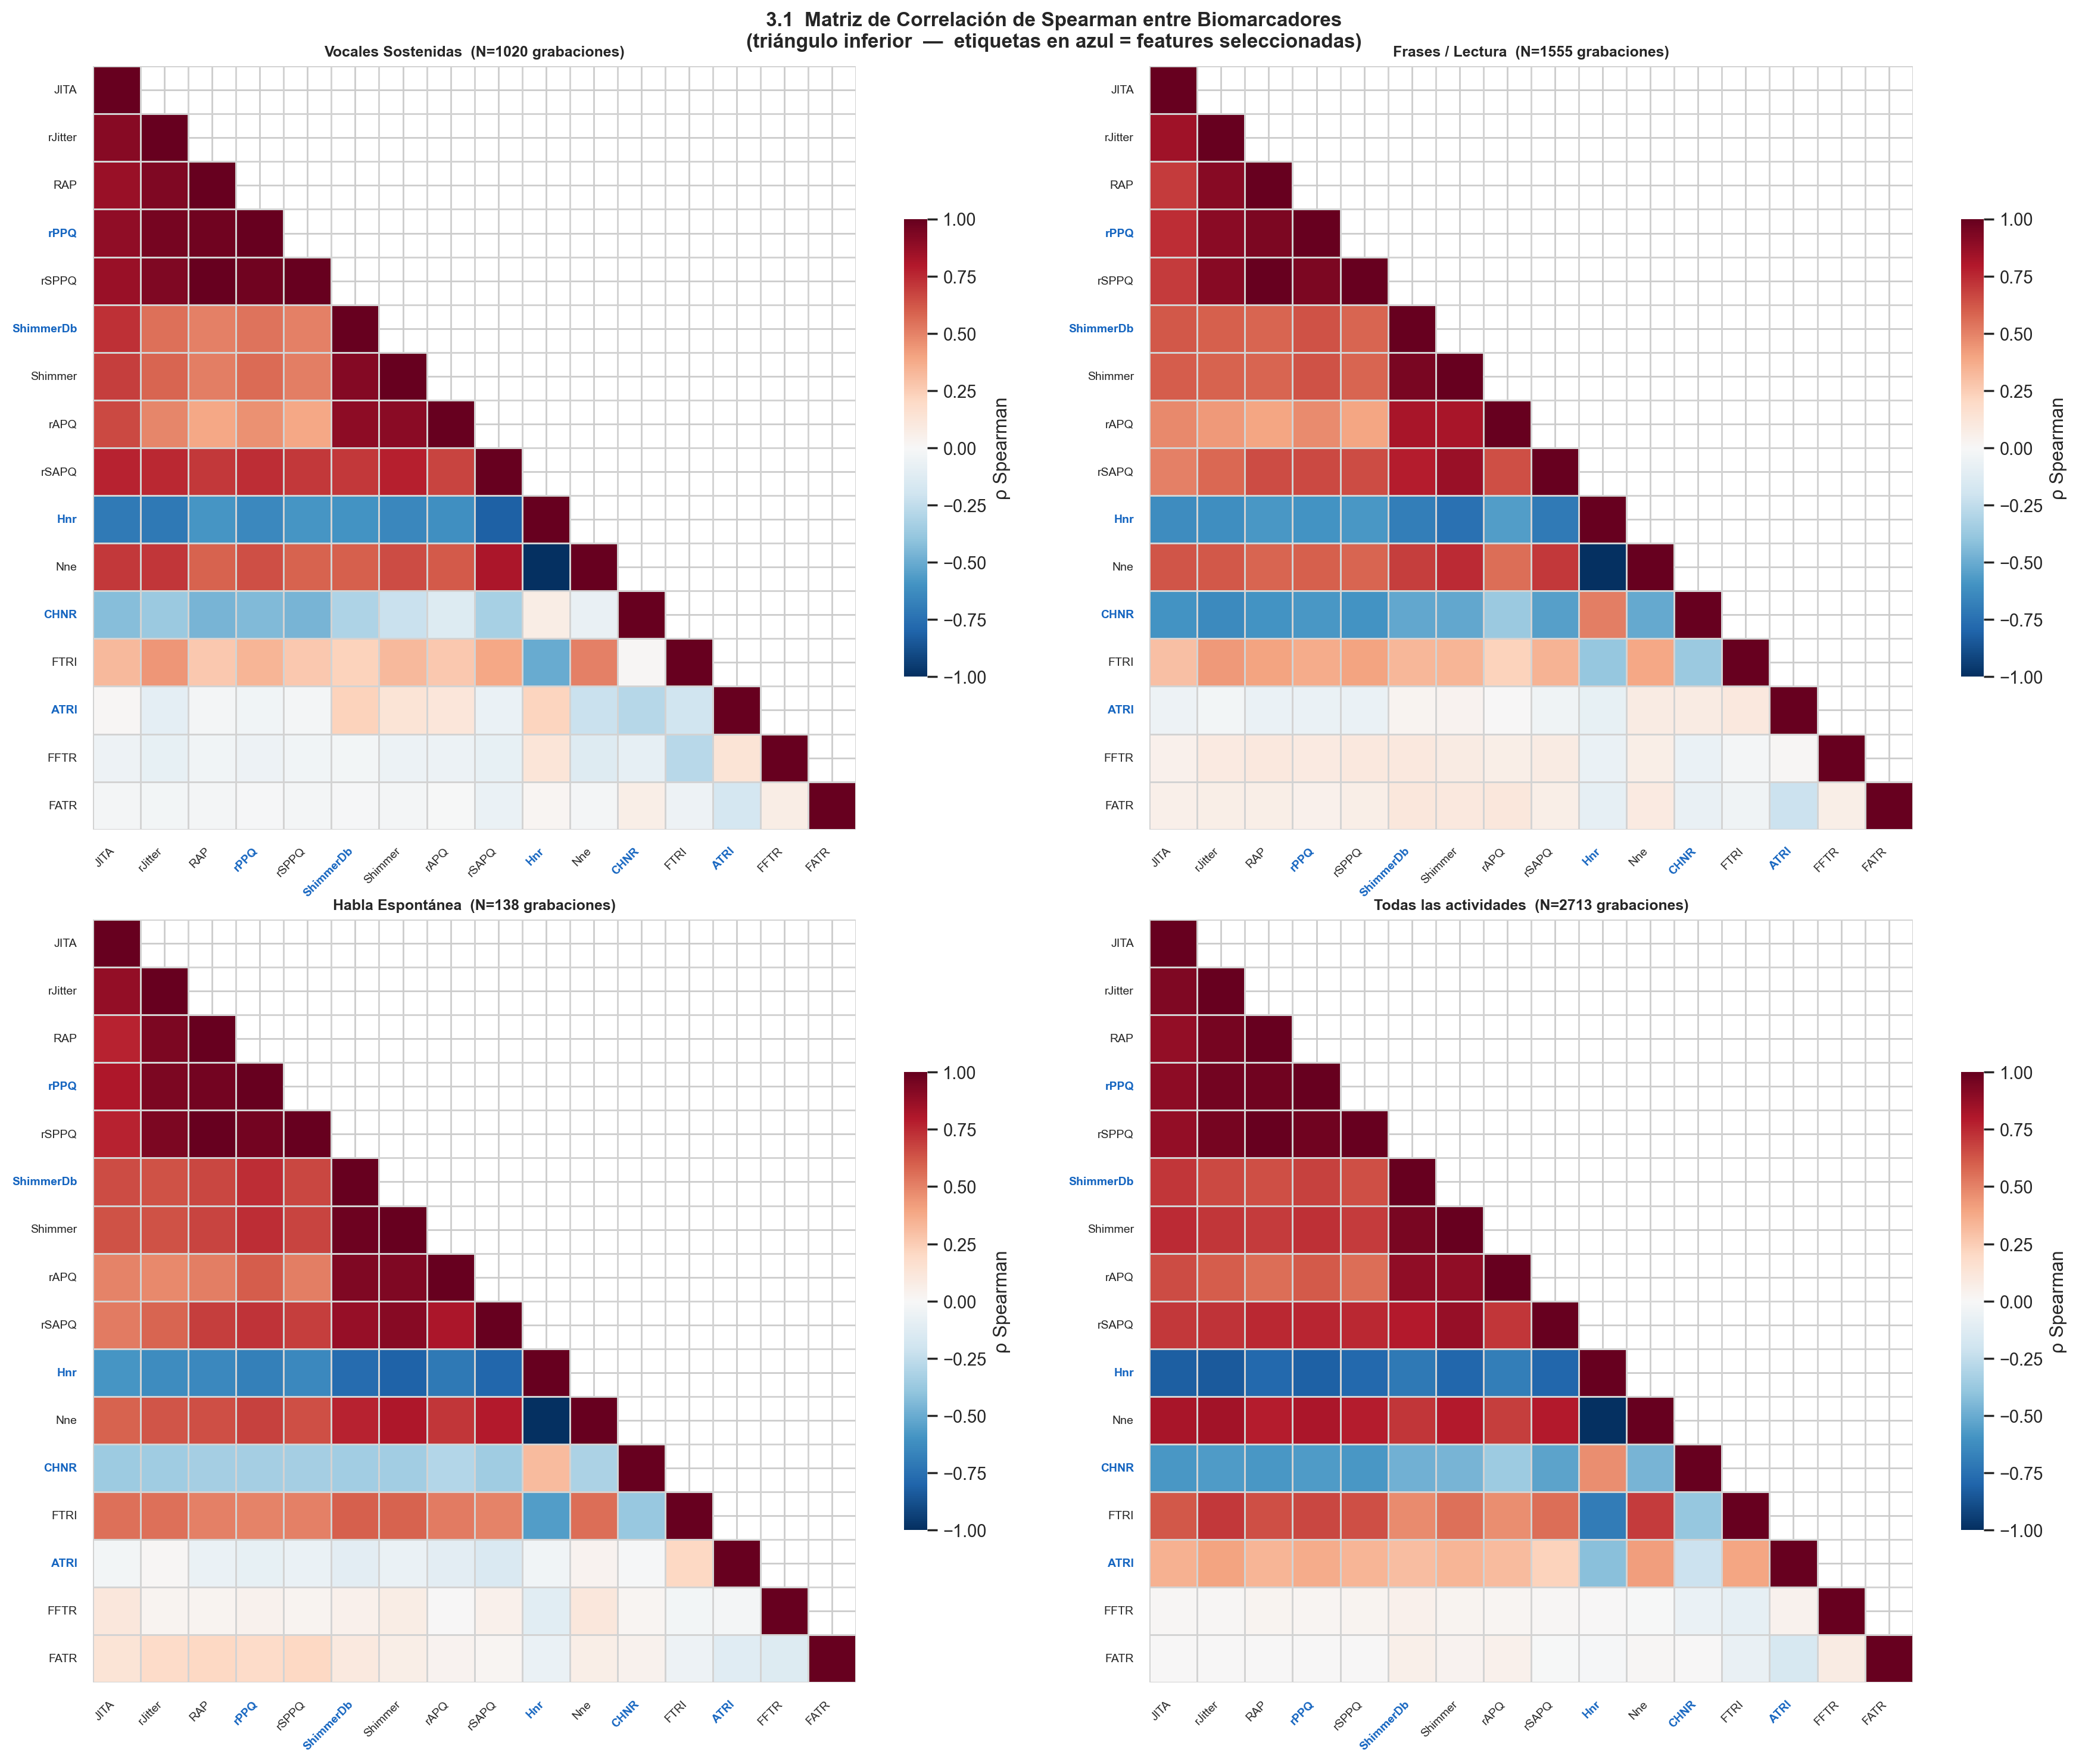
\includegraphics[width=\textwidth, height=0.34\textheight, keepaspectratio]{imagenes/eda/eda_09_corr_features.png}
                \caption{Matriz de correlación de Spearman inter-variable (triángulo inferior). Etiquetas en azul = características seleccionadas.}
                \label{fig:correlacionCcas}
            \end{subfigure}

            \vspace{0.5em}

            \begin{subfigure}[b]{\textwidth}
                \centering
                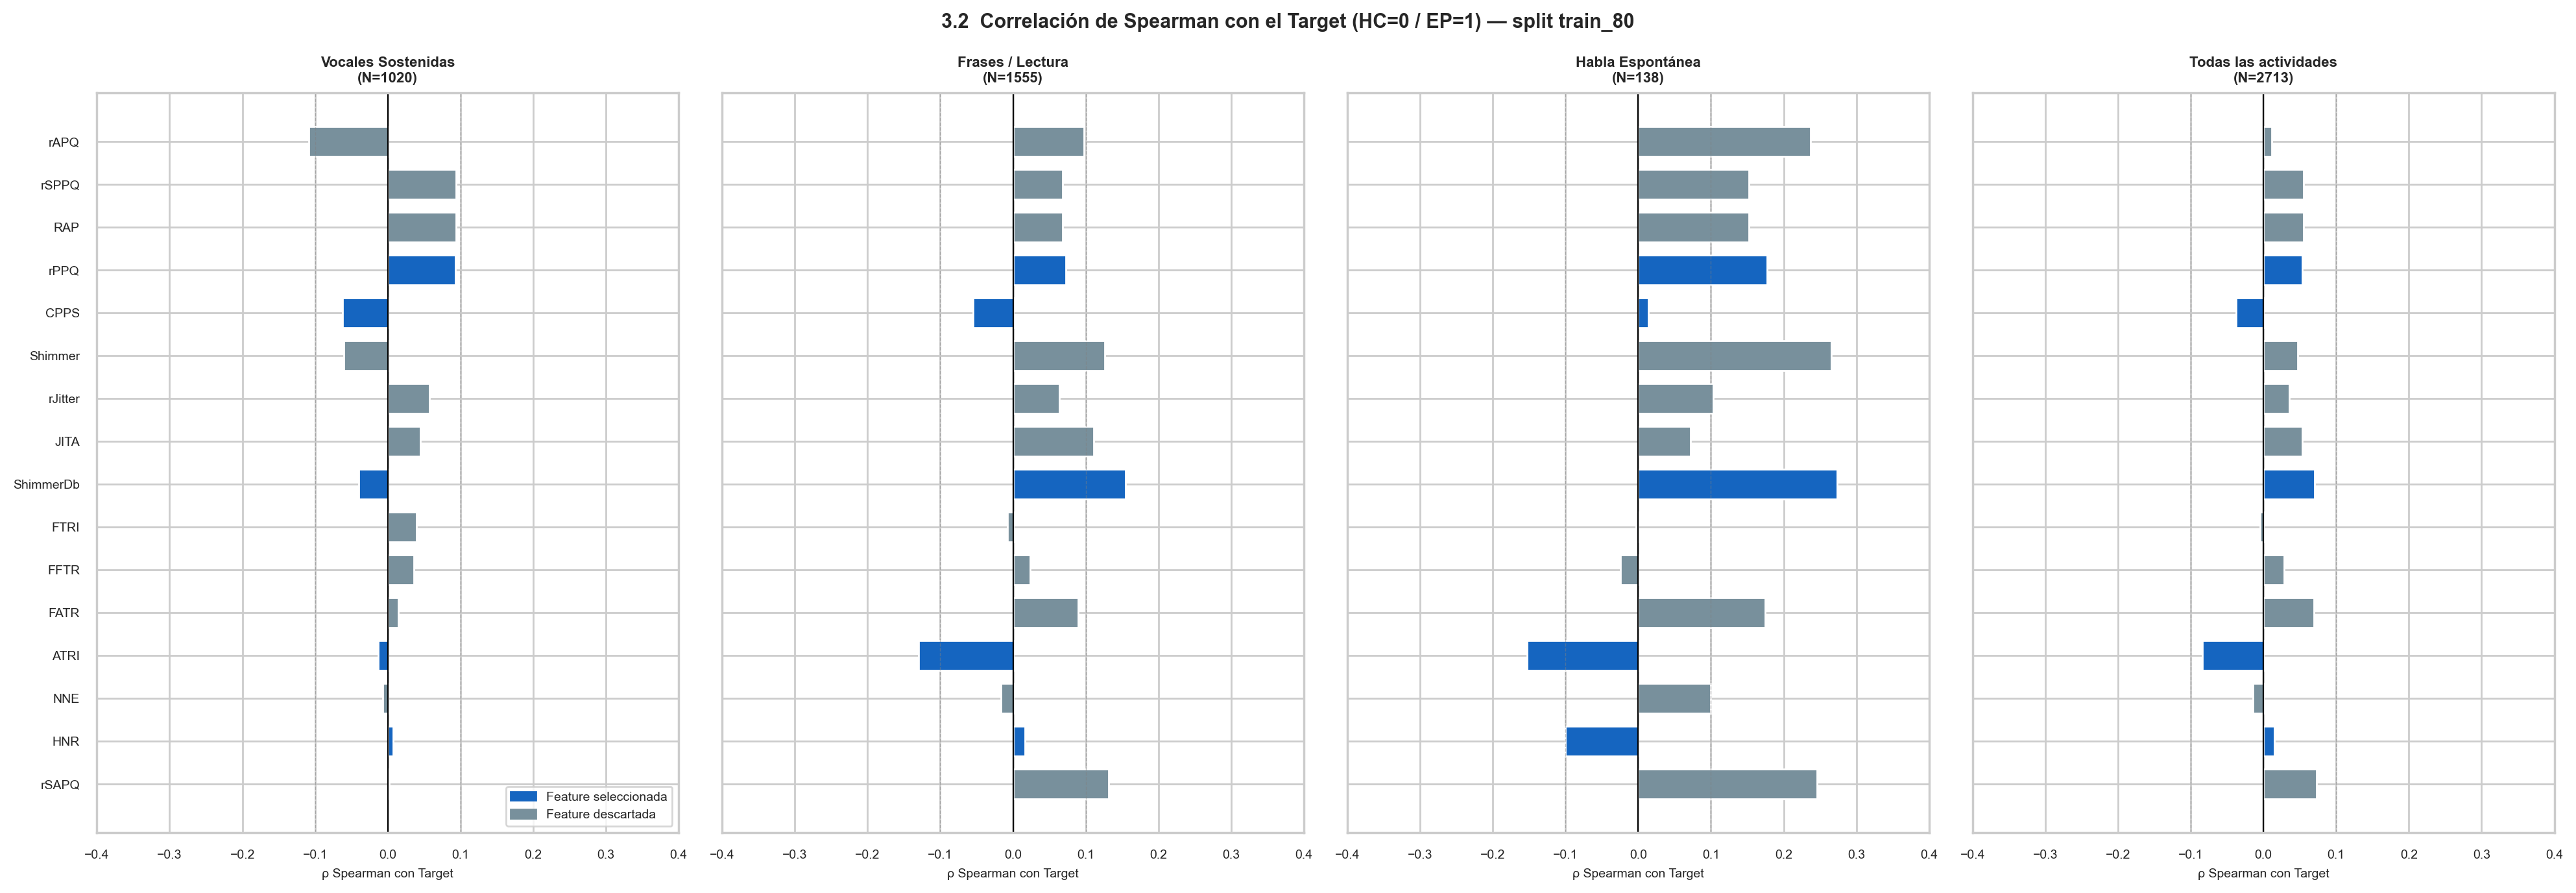
\includegraphics[width=\textwidth, height=0.21\textheight, keepaspectratio]{imagenes/eda/eda_10_corr_target.png}
                \caption{Correlación de Spearman de cada biomarcador con el \textit{Target} (HC\,=\,0 / EP\,=\,1), ordenada por valor absoluto ascendente.}
                \label{fig:correlacionClases}
            \end{subfigure}

            \vspace{0.5em}

            \begin{subfigure}[b]{\textwidth}
                \centering
                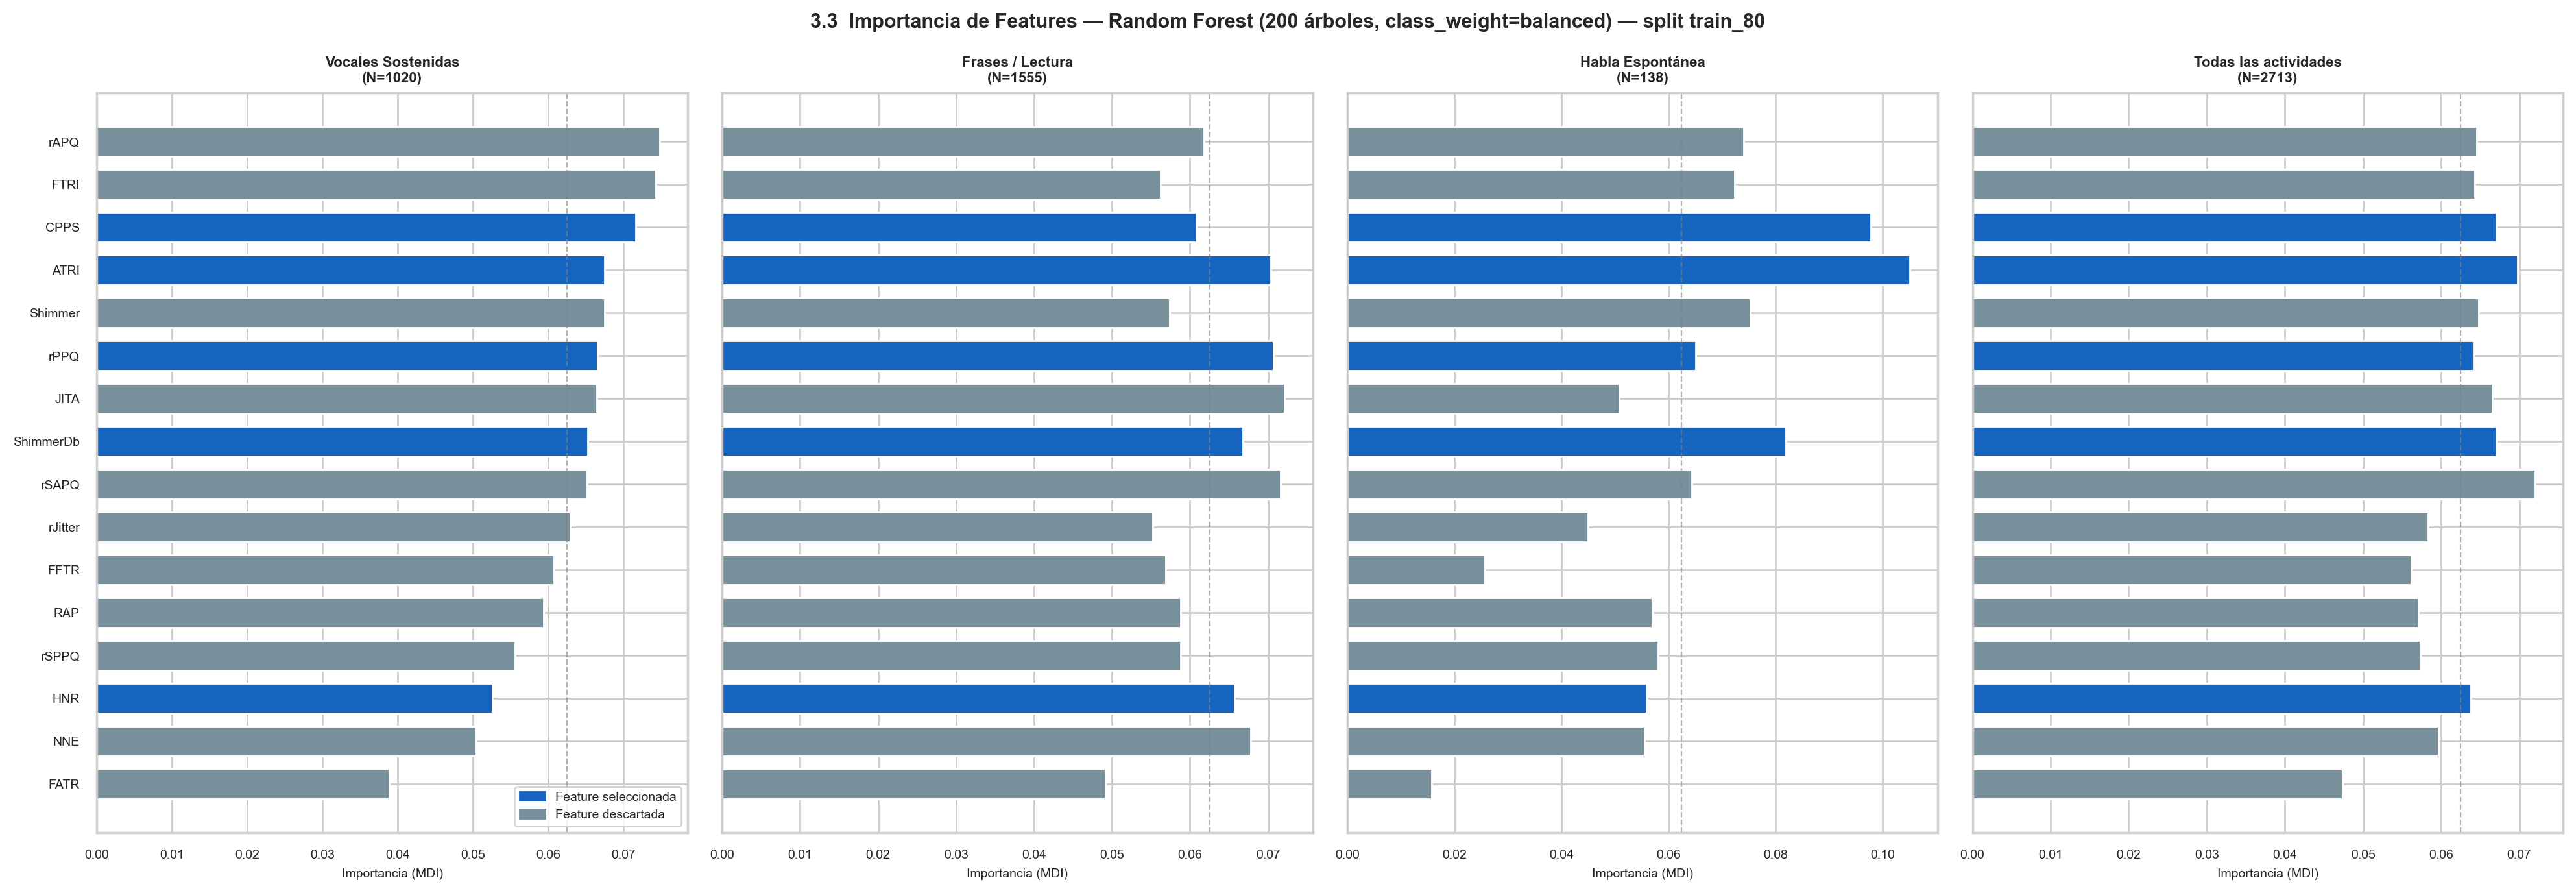
\includegraphics[width=\textwidth, height=0.21\textheight, keepaspectratio]{imagenes/eda/eda_11_rf_importance.png}
                \caption{Importancia predictiva por \textit{Random Forest} (criterio Gini). La línea discontinua marca la importancia uniforme (1/16).}
                \label{fig:pesosRF}
            \end{subfigure}

            \caption{Análisis estadísticos para la selección de características, calculados sobre el \textit{split} de entrenamiento (165 pacientes) y desglosados por actividad de habla: (a)~correlación inter-variable, (b)~correlación univariante con la clase objetivo y (c)~importancia predictiva mediante \textit{Random Forest}. Las barras y etiquetas en azul corresponden a las cinco características finalmente seleccionadas.}
            \label{fig:analisis_seleccion}
        \end{figure}


        \subsection{Análisis Estadístico de los Biomarcadores Acústicos}\label{sec:eda_features}

        Una vez completado el proceso de selección de características, se procedió a realizar un análisis estadístico descriptivo para evaluar la capacidad discriminativa preliminar de las variables seleccionadas. 

        En la Tabla~\ref{tab:medias_acusticas} se presentan las medidas de tendencia central y dispersión (media y desviación típica) de las cinco métricas fundamentales para el conjunto total de grabaciones, segmentadas por grupo diagnóstico.

        \begin{table}[H]
            \centering
            \renewcommand{\arraystretch}{1.3}
            \begin{tabularx}{0.8\textwidth}{>{\raggedright\arraybackslash}X c c}
                \toprule
                \textbf{Biomarcador Acústico} & \textbf{Control Sano (HC)} & \textbf{Parkinson (EP)} \\
                \midrule
                \textbf{rPPQ} & $0.68 \pm 0.43$ & $0.79 \pm 0.70$ \\
                \textbf{ShimmerDb} & $1.08 \pm 0.28$ & $1.12 \pm 0.31$ \\
                \textbf{HNR} & $15.88 \pm 5.42$ & $16.09 \pm 5.88$ \\
                \textbf{CPPS} & $9.79 \pm 2.05$ & $9.62 \pm 2.03$ \\
                \textbf{ATRI} & $10.89 \pm 4.91$ & $9.89 \pm 4.51$ \\
                \bottomrule
            \end{tabularx}
            \caption{Estadística descriptiva (Media $\pm$ Desviación Típica) de las características acústicas seleccionadas para sujetos de Control (HC) y pacientes con Parkinson (EP).}
            \label{tab:medias_acusticas}
        \end{table}

        A nivel clínico, se observa empíricamente un incremento en las medidas de inestabilidad vocal (rPPQ y ShimmerDb) en el grupo patológico, congruente con la pérdida de control neuromotor característica de la disartria hipocinética. Asimismo, el índice de temblor de amplitud (ATRI) muestra una alteración en su distribución. 

        El análisis estadístico exhaustivo de la totalidad de las variables extraídas inicialmente, así como las representaciones gráficas de sus distribuciones, diagramas de violín y matrices de dispersión, se encuentran detallados de forma íntegra en el \textbf{\hyperref[app:eda]{Apéndice C}}.


            

        \subsection{Generación de representaciones acústicas para Deep Learning}
        \label{sec:espectrogramas}

        A diferencia de los algoritmos de aprendizaje automático clásico, las arquitecturas de aprendizaje profundo (Deep Learning) basadas en Redes Neuronales Convolucionales (CNN) destacan por su capacidad para extraer características latentes directamente desde matrices bidimensionales. Por consiguiente, se diseñó un pipeline paralelo para transformar las señales acústicas unidimensionales en representaciones de tiempo-frecuencia, específicamente \textbf{espectrogramas en escala Mel}.

        La elección de la escala Mel frente a un espectrograma lineal estándar radica en su naturaleza logarítmica, la cual emula con mayor fidelidad la resolución perceptiva del sistema auditivo humano \cite{stevens1937}. Esta compresión del espectro otorga mayor peso y resolución a las frecuencias bajas e intermedias, banda donde residen los formantes principales de la voz humana y las micro-fluctuaciones asociadas a la disartria parkinsoniana.

        El proceso de conversión acústico-visual se llevó a cabo aplicando la Transformada Corta de Fourier (STFT, por sus siglas en inglés) sobre las señales previamente preprocesadas a 16 kHz, implementando el flujo a través de la librería \textit{librosa} \cite{mcfee2015}. Los hiperparámetros matemáticos empleados para la generación computacional de los espectrogramas fueron los siguientes:

        \begin{itemize}
            \item \textbf{Tamaño de la ventana (n\_fft):} Se fijó en 512 muestras, proporcionando una resolución frecuencial adecuada para aislar perturbaciones micromotoras.
            \item \textbf{Desplazamiento temporal (hop\_length):} Se calculó dinámicamente como el 3\,\% de la frecuencia de muestreo (aproximadamente 480 muestras a 16 kHz) entre ventanas consecutivas.
            \item \textbf{Función de enventanado (\textit{Window function}):} Se aplicó la ventana estándar de Hann (por defecto en la implementación matemática de la librería) para mitigar las fugas espectrales (\textit{spectral leakage}) en los extremos de cada segmento.
            \item \textbf{Filtros Mel (n\_mels):} El banco de filtros se configuró para proyectar el espectro sobre 65 bandas Mel.
        \end{itemize}

        Posteriormente, la matriz de densidad espectral de potencia resultante ($S$) fue convertida a una escala logarítmica de decibelios (dB) siguiendo la ecuación $S_{dB} = 10 \cdot \log_{10}(S / S_{ref})$, tomando como referencia la amplitud máxima. 

        En la \autoref{fig:ejemplo_espectrograma} se ilustra una comparativa visual entre los espectrogramas extraídos para un paciente patológico y un sujeto de control.

        \begin{figure}[H]
        \centering
        % Espectrograma Sujeto Sano
        \begin{subfigure}[b]{0.48\textwidth}
            \centering
            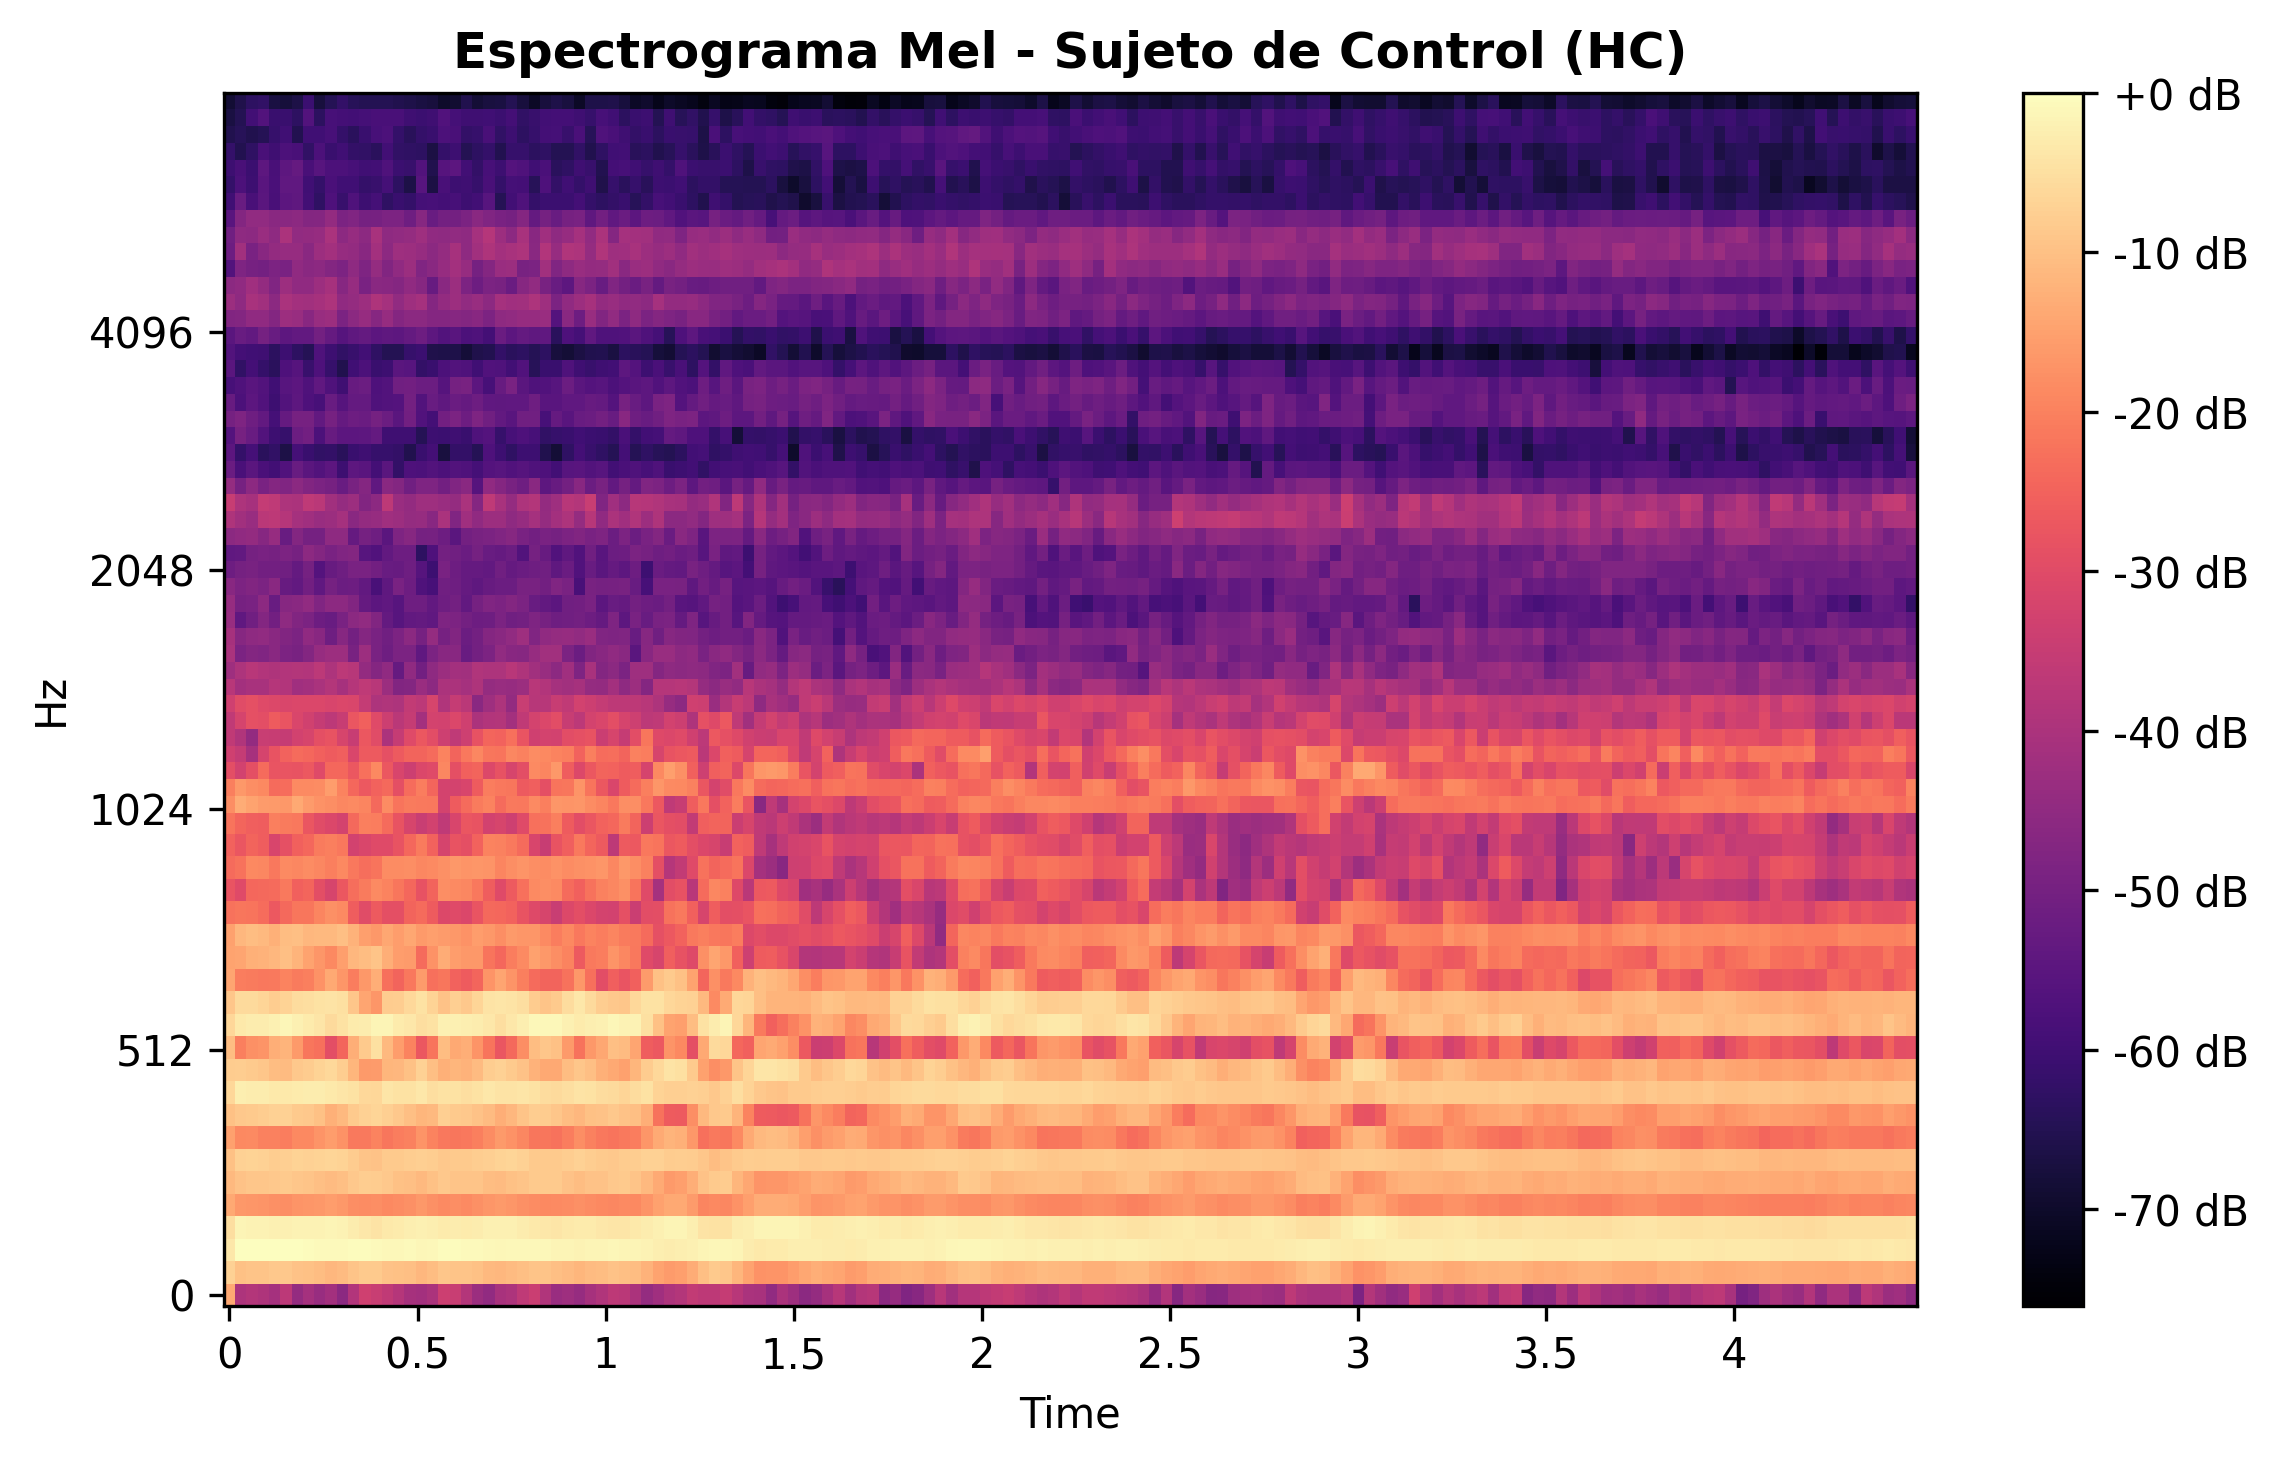
\includegraphics[width=\textwidth]{imagenes/espectrograma_sano.png}
            \caption{Sujeto de Control (HC)}
            \label{fig:spec_sano}
        \end{subfigure}
        \hfill
        % Espectrograma Paciente Parkinson
        \begin{subfigure}[b]{0.48\textwidth}
            \centering
            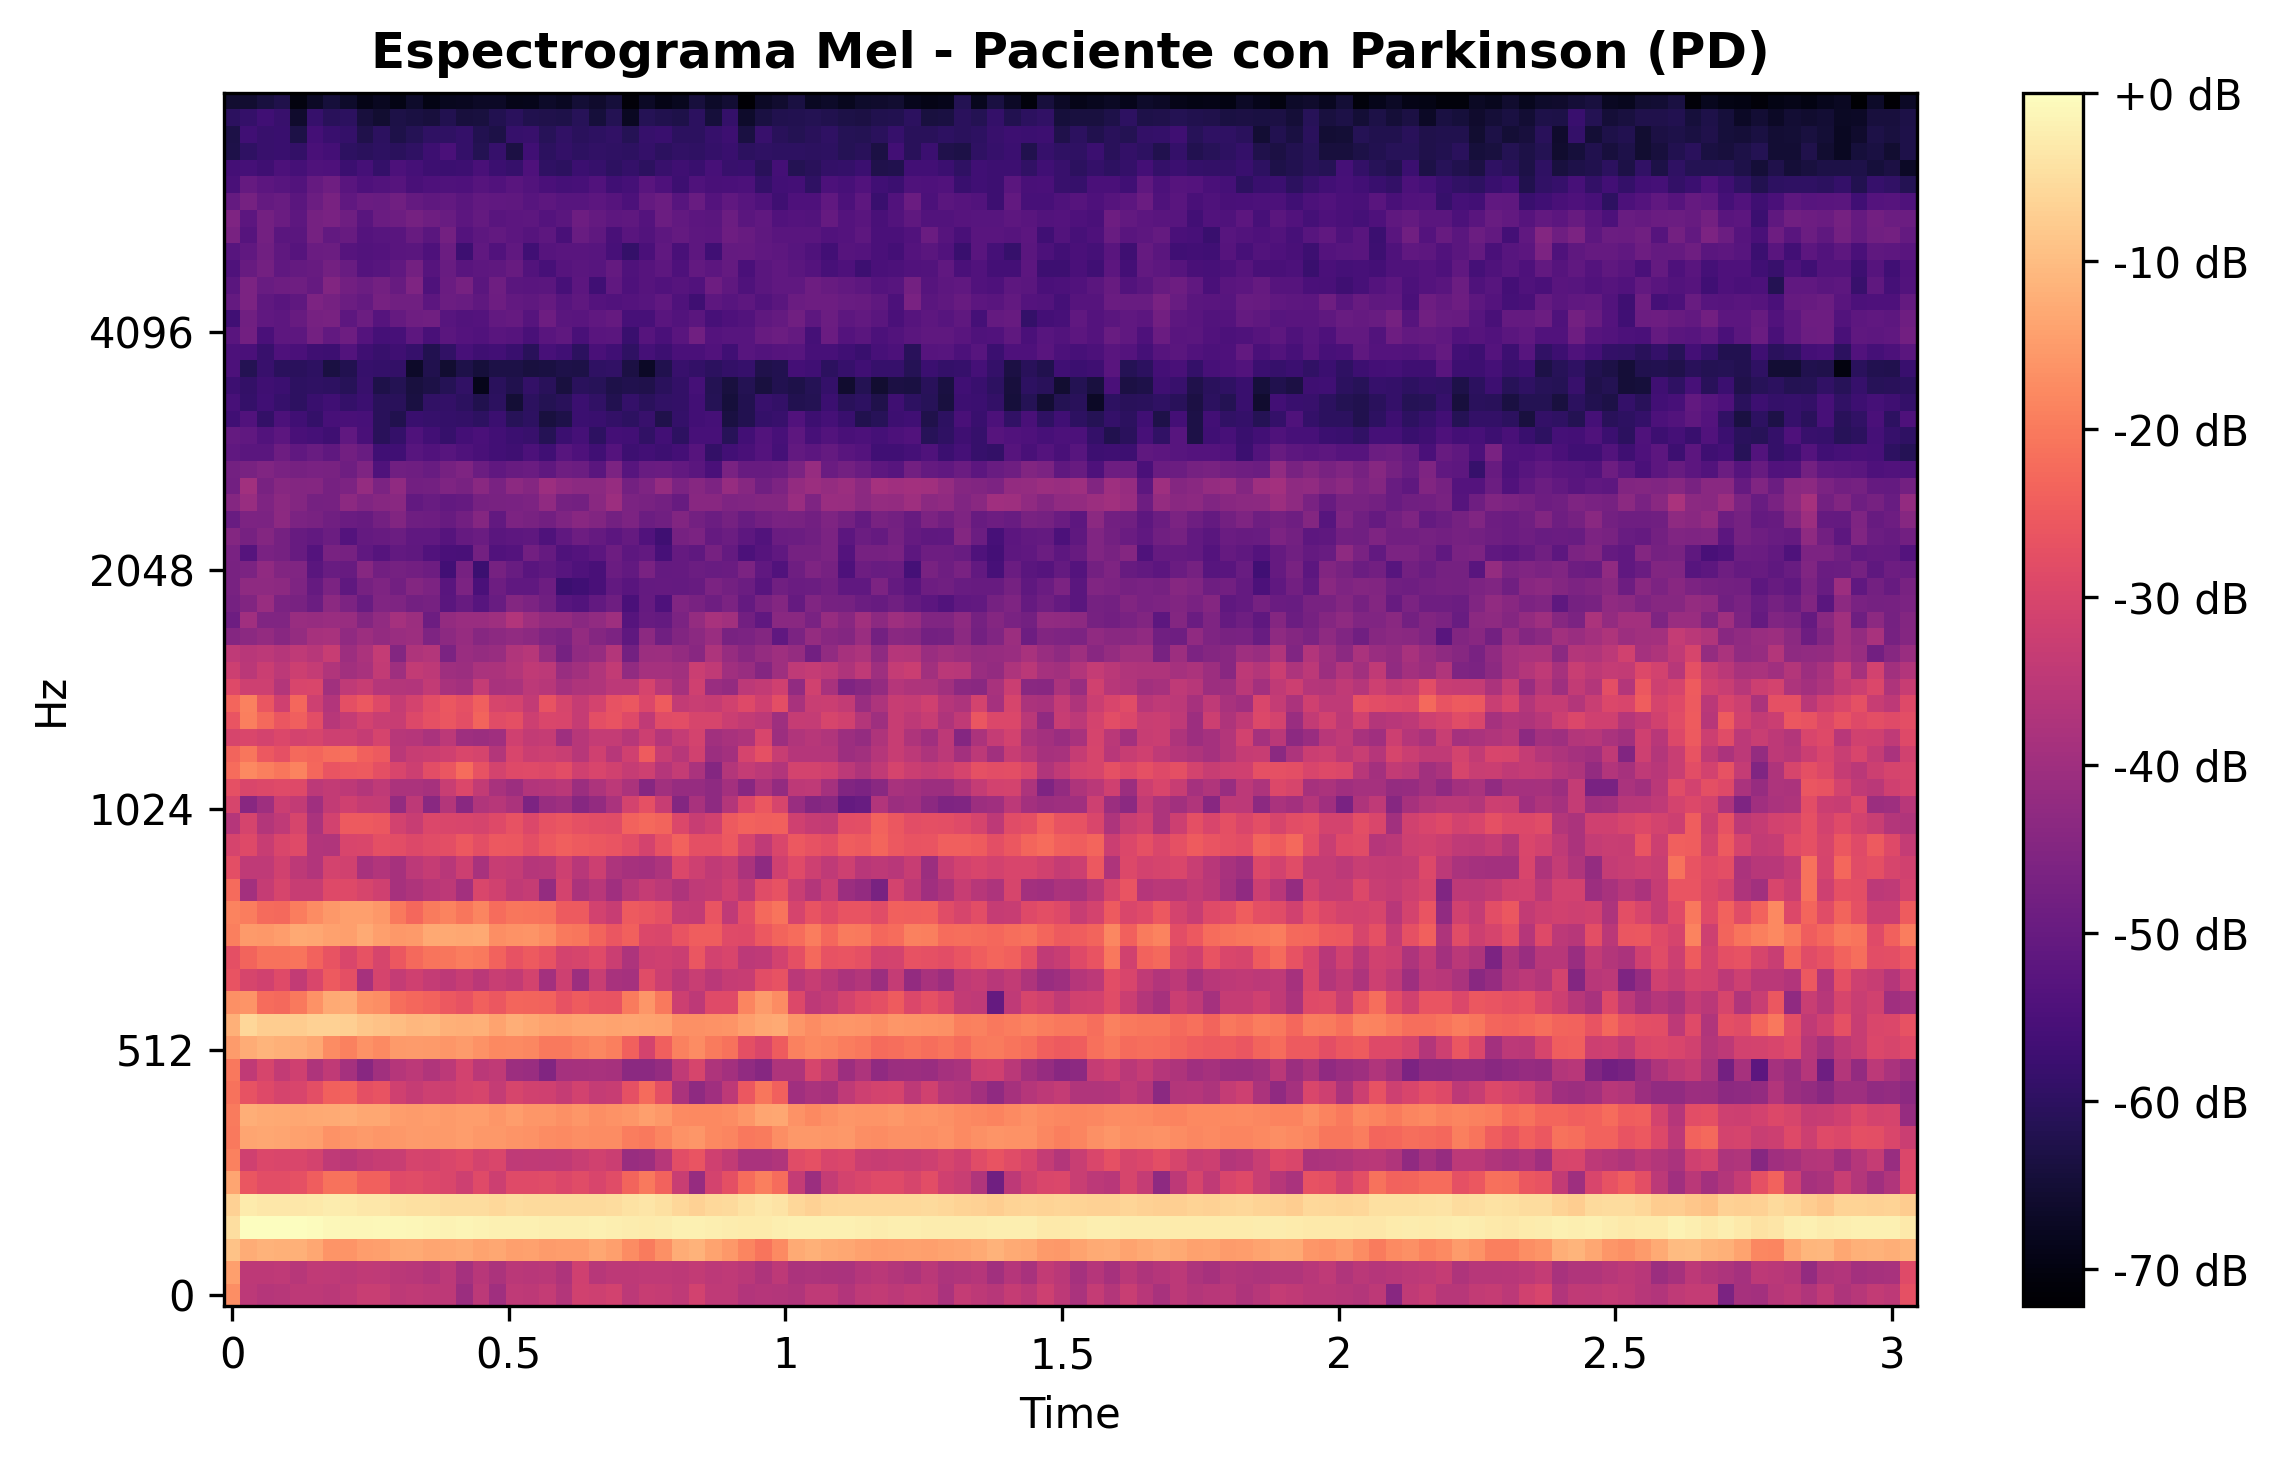
\includegraphics[width=\textwidth]{imagenes/espectrograma_parkinson.png}
            \caption{Paciente con Parkinson (PD)}
            \label{fig:spec_parkinson}
        \end{subfigure}
        
        \caption{Comparativa visual de espectrogramas en escala Mel generados con un banco de 65 filtros y una ventana de 512 muestras. Se observa la representación acústico-visual de un sujeto de control sano frente a las alteraciones y micro-fluctuaciones típicas de un paciente con Enfermedad de Parkinson.}
        \label{fig:ejemplo_espectrograma}
    \end{figure}


    \subsection{Extracción de embeddings acústicos mediante Wav2Vec 2.0}

    De forma complementaria a la extracción de características acústicas manuales y a la generación de espectrogramas, se exploró el uso de modelos fundacionales de aprendizaje profundo para la obtención de representaciones latentes de alto nivel (\textit{embeddings}). Para este propósito, se implementó la arquitectura \textbf{Wav2Vec 2.0} \cite{baevski2020}, un modelo de vanguardia desarrollado por Meta AI basado en aprendizaje auto-supervisado (\textit{Self-Supervised Learning}).

    A diferencia de las métricas clásicas, Wav2Vec 2.0 procesa la forma de onda cruda para extraer un contexto acústico denso, lo que resulta especialmente útil para capturar las sutilezas neuromotoras de la voz patológica sin necesidad de un etiquetado previo alineado fonéticamente \cite{baevski2020}. Se seleccionó específicamente la variante preentrenada \texttt{jonatasgrosman/wav2vec2-large-xlsr-53-spanish}, una adaptación del modelo XLSR-53 de Meta AI preentrenada en 53 idiomas y ajustada finamente (\textit{fine-tuned}) sobre corpus de habla espontánea en español. Esta elección responde a la naturaleza lingüística de los corpus clínicos empleados (NeuroVoz y PC-GITA, ambos en castellano), garantizando que las representaciones latentes extraídas capturen las propiedades fonéticas específicas del español sin depender de un preentrenamiento exclusivamente multilingüe.

    El pipeline de extracción automatizada se diseñó haciendo uso del ecosistema PyTorch y la librería \textit{Transformers}. El flujo de procesamiento por cada archivo de audio siguió las siguientes etapas matemáticas y computacionales:

    \begin{itemize}
        \item \textbf{Acondicionamiento de la señal:} Las muestras se cargaron a través de \textit{torchaudio}, forzando la conversión a formato mono (promediando los canales espaciales). Seguidamente, se aplicó un remuestreo dinámico a 16 kHz, requisito arquitectónico estricto impuesto por los datos de preentrenamiento del modelo Wav2Vec 2.0 \cite{wolfTransformersStateoftheArtNatural2020}.
        
        \item \textbf{Inferencia y estado latente:} La señal normalizada se introdujo en el modelo en modo de evaluación (\texttt{model.eval()}). Para garantizar la eficiencia en memoria y acelerar el cómputo en la unidad de procesamiento gráfico (GPU), el cálculo de tensores se aisló del grafo de retropropagación (\texttt{torch.no\_grad()}) \cite{paszke2019}.
        
        \item \textbf{Agrupamiento Global (\textit{Global Average Pooling}):} La arquitectura devuelve una secuencia temporal de estados ocultos correspondientes a la última capa del \textit{Transformer} (\textit{last\_hidden\_state}) \cite{wolfTransformersStateoftheArtNatural2020}. Para colapsar esta secuencia temporal (de longitud variable según la duración del audio) en un único vector de longitud fija por paciente, se aplicó la media aritmética sobre el eje temporal. 
    \end{itemize}

    El resultado de esta operación (\textit{pooling}) proyecta cada grabación de voz en un espacio vectorial continuo de \textbf{1024 dimensiones}. Este vector resultante codifica de forma abstracta las propiedades fonéticas y prosódicas del locutor, y fue exportado en formato tabular para su posterior ingestión como vector de características (\textit{feature vector}) en los modelos predictivos de Machine Learning.      

    \section{Entorno tecnológico (Hardware, librerías de Python)}
    \subsection{Hardware utilizado}
        Los experimentos, el procesamiento de las bioseñales y el entrenamiento de los modelos fueron ejecutados en dos estaciones de trabajo independientes. Esta división permitió distribuir la carga computacional según los exigentes requisitos de memoria de las distintas arquitecturas empleadas:

        \begin{itemize}
            \item \textbf{Estación de Trabajo 1 (Preprocesamiento y ML Clásico):} Empleada principalmente para la limpieza de las señales acústicas, la extracción de características manuales y el entrenamiento de los algoritmos de Machine Learning tradicional (KNN y XGBoost).
            \item \textbf{Estación de Trabajo 2 (Deep Learning y Foundation Models):} Dedicada de forma exclusiva a la generación de espectrogramas Mel, la extracción de representaciones latentes mediante Wav2Vec 2.0 y el entrenamiento de la arquitectura ResNet18, aprovechando una mayor capacidad de memoria VRAM para el cálculo matricial y tensorial.
        \end{itemize}

        \begin{table}[H]
            \centering
            \label{tab:hardware}
            \renewcommand{\arraystretch}{1.3}
            \begin{tabularx}{\textwidth}{>{\raggedright\arraybackslash}p{3.5cm} X X}
                \toprule
                \textbf{Componente} & \textbf{Estación de Trabajo 1} & \textbf{Estación de Trabajo 2} \\
                \midrule
                \textbf{Procesador (CPU)} & Intel\textsuperscript{\textregistered} Core\textsuperscript{\texttrademark} i7-12650H \newline (10 núcleos, 16 hilos) 2.30 GHz & Intel\textsuperscript{\textregistered} Core\textsuperscript{\texttrademark} i7-13700H \newline (14 núcleos, 20 hilos) 2.30 GHz \\
                \textbf{Memoria RAM} & 16 GB SODIMM a 3200 MT/s & 16 GB SODIMM a 5200 MT/s \\
                \textbf{Tarjeta Gráfica} & NVIDIA\textsuperscript{\textregistered} GeForce\textsuperscript{\textregistered} RTX\textsuperscript{\texttrademark} 3050 \newline Laptop GPU (4 GB VRAM) & NVIDIA\textsuperscript{\textregistered} GeForce\textsuperscript{\textregistered} RTX\textsuperscript{\texttrademark} 4060 \newline Laptop GPU (8 GB VRAM)  \\
                \textbf{Almacenamiento} & 512 GB SSD (WD PC SN740) & 1 TB SSD (SAMSUNG MZVL21T0HCLR) \\
                \textbf{Sistema Operativo} & Windows 11 Pro (64 bits) & Windows 11 Home (64 bits) \\
                \bottomrule
            \end{tabularx}
            \caption{Especificaciones de hardware de los equipos utilizados para el procesamiento y entrenamiento de los modelos.}
        \end{table}


    \subsection{Librerías de Python utilizadas}

        Para el desarrollo de este proyecto se ha establecido un entorno de trabajo basado en Python. La gestión de los paquetes y las dependencias se ha realizado utilizando \textbf{uv}, un gestor de proyectos moderno escrito en Rust que destaca por su extrema rapidez y su capacidad para garantizar la reproducibilidad de los experimentos.

        Debido a la gran cantidad de librerías involucradas en el entrenamiento de los modelos y el despliegue del sistema, en la \autoref{tab:librerias_proyecto} se resumen las herramientas principales, agrupadas según su propósito dentro del flujo de trabajo.

        
        \begin{table}[htbp]
            \centering
            \begin{tabular}{@{}llp{8cm}@{}}
                \toprule
                \textbf{Librería / Herramienta} &  \textbf{Propósito en el proyecto} \\
                \midrule
                
                \multicolumn{2}{c}{\textbf{Gestión de Entorno y Backend}} \\
                \midrule
                uv & Gestor de paquetes y dependencias ultrarrápido escrito en Rust. \\
                FastAPI \& Uvicorn & Desarrollo y despliegue del servidor API REST. \\
                \midrule
                
                \multicolumn{2}{c}{\textbf{Deep Learning y Machine Learning}} \\
                \midrule
                Ecosistema PyTorch & Framework principal (incluye TorchAudio y TorchVision). \\
                Transformers \& TIMM & Implementación de modelos de lenguaje y visión avanzados. \\
                XGBoost \& scikit-learn & Algoritmos de aprendizaje automático tradicional y métricas. \\
                SHAP & Explicabilidad e interpretabilidad de los modelos de IA. \\
                \midrule
                
                \multicolumn{2}{c}{\textbf{Procesamiento de Audio y Datos}} \\
                \midrule
                Librosa, Parselmouth \& NoiseReduce & Carga, limpieza y extracción de características acústicas. \\
                Pandas, NumPy \& SciPy & Manipulación de datos tabulares y cálculo científico. \\
                Matplotlib \& Seaborn & Visualización de datos y generación de gráficas. \\
                \bottomrule
            \end{tabular}
            \caption{Principales librerías y herramientas de software utilizadas en el proyecto agrupadas por categoría.}
            \label{tab:librerias_proyecto}
        \end{table}

        
        Como se puede observar, el núcleo del proyecto se apoya fuertemente en el ecosistema de PyTorch para el aprendizaje profundo, complementado con FastAPI para la creación de la interfaz de comunicación. 

        Para mantener la claridad del documento, el listado exhaustivo y completo de todas las dependencias del proyecto, junto con sus versiones exactas y subdependencias (reflejadas en el entorno virtual generado por \texttt{uv}), se encuentra detallado en el \textbf{\hyperref[app:anexo_a]{Apéndice~\ref{app:anexo_a}}}.



        
    \section{Métricas de evaluación del rendimiento}
\label{sec:metricas}

La evaluación de modelos predictivos en el ámbito clínico y biomédico requiere un análisis exhaustivo que trascienda la simple tasa de aciertos (\textit{Accuracy}). Dado el impacto crítico de los falsos negativos (pacientes con Parkinson no detectados) y los falsos positivos (sujetos sanos diagnosticados erróneamente), el rendimiento de los algoritmos se evaluó a través de la matriz de confusión, extrayendo las métricas estadísticas estándar para tareas de clasificación binaria \cite{sokolova2009}. 

En la formulación matemática, $TP$ representa los Verdaderos Positivos, $TN$ los Verdaderos Negativos, $FP$ los Falsos Positivos y $FN$ los Falsos Negativos.

\begin{itemize}
    \item \textbf{Exactitud (\textit{Accuracy}):} Mide la proporción global de predicciones correctas sobre el total de la muestra. Aunque ofrece una visión general, puede resultar engañosa en conjuntos de datos desbalanceados.
    $$Accuracy = \frac{TP + TN}{TP + TN + FP + FN}$$
    
    \item \textbf{Sensibilidad o \textit{Recall} (\textit{True Positive Rate}):} Es la métrica clínica más crítica en esta investigación. Cuantifica la capacidad del modelo para identificar correctamente a los pacientes que realmente padecen la enfermedad de Parkinson, minimizando los casos que pasan desapercibidos.
    $$Sensibilidad = \frac{TP}{TP + FN}$$
    
    \item \textbf{Especificidad (\textit{True Negative Rate}):} Evalúa la proporción de sujetos de control sanos que son correctamente identificados como tales. Una alta especificidad asegura que no se diagnostica erróneamente la patología a personas sanas.
    $$Especificidad = \frac{TN}{TN + FP}$$

    \item \textbf{Exactitud Balanceada (\textit{Balanced Accuracy}):} Definida como el promedio de la tasa de aciertos en cada clase individual. Evita que un modelo parezca bueno cuando solo acierta en la clase más abundante.
    $$Balanced Accuracy = \frac{Sensibilidad + Especificidad}{2}$$
    
    \item \textbf{Precisión (\textit{Positive Predictive Value}):} Indica la proporción de pacientes diagnosticados con Parkinson por el modelo que realmente padecen la enfermedad.
    $$Precision = \frac{TP}{TP + FP}$$
    
    \item \textbf{F1-Score:} Representa la media armónica entre la Precisión y la Sensibilidad. Es una métrica de un solo valor (\textit{single-number evaluation metric}) robusta frente al desbalanceo de clases, ya que penaliza los modelos que sacrifican una métrica en favor de la otra.
    $$F1 = 2 \cdot \frac{Precision \cdot Sensibilidad}{Precision + Sensibilidad}$$
\end{itemize}

De forma complementaria, el poder discriminatorio probabilístico de los modelos se evaluó mediante la \textbf{Curva ROC} (\textit{Receiver Operating Characteristic}) \cite{fawcett2006}, que grafica la Sensibilidad frente a la tasa de falsos positivos ($1 - Especificidad$) en diversos umbrales de decisión. Para cuantificar esta curva, se calculó el \textbf{Área Bajo la Curva (AUC-ROC)}, donde un valor de 1.0 indica un modelo perfecto y un valor de 0.5 equivale a una predicción aleatoria.

    \chapter{Diseño y Desarrollo de los Modelos}\label{ch:diseno}

En este capítulo se describe exhaustivamente el diseño, la configuración experimental y la arquitectura de los modelos predictivos desarrollados. El flujo de trabajo abarca desde la implementación de algoritmos de Machine Learning tradicional hasta el ajuste de modelos de representación profunda, garantizando en todo momento la robustez estadística y la generalización clínica de los resultados.

    \section{Configuración experimental y estrategias de entrenamiento}\label{sec:configuracion_experimental}

Para asegurar la validez de los modelos predictivos y evitar el sobreajuste (\textit{overfitting}), se diseñó una estrategia de partición de datos y validación cruzada rigurosa, adaptada a la naturaleza jerárquica de los corpus de voz.

\subsection{Partición de los datos y prevención del \textit{Data Leakage}}
La unidad muestral en este estudio no es la grabación individual, sino el paciente. Dado que cada sujeto aportó múltiples muestras de audio correspondientes a distintas tareas fonatorias (vocales, frases y habla espontánea), un muestreo aleatorio simple habría provocado la contaminación del conjunto de prueba con patrones biométricos aprendidos en el conjunto de entrenamiento, un fenómeno conocido como \textit{Data Leakage}.

Para evitarlo, la partición de los datos se realizó estrictamente a nivel de paciente (agrupando por el identificador único del locutor). Se aplicó una división del tipo \textit{Hold-out}, reservando un 80\% de los sujetos para la fase de construcción del modelo (entrenamiento y validación cruzada) y el 20\% restante como conjunto de prueba externo. Adicionalmente, esta partición se ejecutó de forma estratificada utilizando una clave combinada que integraba la clase objetivo (Parkinson o Control) y el origen del corpus (NeuroVoz o PC-GITA), garantizando así el balanceo epidemiológico en ambas particiones.

\subsection{Validación Cruzada (\textit{Cross-Validation})}
Sobre el conjunto de entrenamiento (80\% de los datos), se implementó una estrategia de validación cruzada para la optimización de los hiperparámetros. Se empleó el algoritmo \textit{Stratified Group K-Fold} con $K=5$ particiones (\textit{folds}). 

Este enfoque asegura dos propiedades matemáticas fundamentales durante cada iteración:
\begin{enumerate}
    \item \textbf{Agrupación estricta:} Ninguna grabación de un mismo paciente aparece simultáneamente en el \textit{fold} de entrenamiento y en el de validación.
    \item \textbf{Estratificación:} Se mantiene la proporción original de la variable objetivo en cada partición, mitigando los sesgos por desbalanceo de clases.
\end{enumerate}

\subsection{Optimización de umbral de decisión (Estadístico de Youden)}
De forma predeterminada, los clasificadores binarios establecen el umbral de decisión en una probabilidad de 0.5. Sin embargo, en escenarios de diagnóstico clínico, este valor rara vez es el óptimo.

Para calibrar los modelos, se separó un 20\% interno del conjunto de entrenamiento exclusivo para validación. Las predicciones probabilísticas de las grabaciones se agregaron calculando la media aritmética por paciente. Sobre estas probabilidades agregadas, se aplicó la curva ROC y se calculó empíricamente el umbral óptimo maximizando el estadístico $J$ de Youden \cite{youden1950}, definido matemáticamente como:

$$J = Sensibilidad + Especificidad - 1$$

O, equivalentemente en términos de tasas:

$$J = TPR - FPR$$

Donde $TPR$ representa la tasa de verdaderos positivos (Sensibilidad) y $FPR$ la tasa de falsos positivos ($1 - Especificidad$). El valor probabilístico de corte que maximizó $J$ fue el empleado para la binarización de las predicciones en el conjunto de prueba externo.

\subsection{Enfoque Multi-Tarea y Modelado Específico por Actividad}\label{sec:multitarea}

A nivel clínico, las alteraciones neuromotoras producidas por la disartria en la Enfermedad de Parkinson no se manifiestan de manera uniforme en todas las tareas del habla. La fonación sostenida de una vocal aísla la vibración mecánica de las cuerdas vocales, mientras que la repetición de frases o el habla espontánea introducen variables complejas como la prosodia, la competencia velofaríngea y la carga cognitiva.

Por consiguiente, mezclar todas las grabaciones en un único conjunto de entrenamiento destruiría la varianza biológica propia de cada prueba. Para preservar esta integridad y evaluar el potencial diagnóstico de cada subsistema, el pipeline de entrenamiento se ejecutó bajo un enfoque multi-tarea. Se instanciaron y evaluaron de forma completamente independiente cuatro variantes para cada algoritmo de Inteligencia Artificial (KNN, XGBoost y ResNet18), segmentadas según la actividad fonatoria de entrada:

\begin{itemize}
    \item \textbf{Modelo de Vocales Sostenidas (\textit{vocal}):} Entrenamiento restringido a grabaciones de fonación pura, diseñado para identificar anomalías en la inestabilidad de la frecuencia y la amplitud (Jitter y Shimmer).
    \item \textbf{Modelo de Frases y Lectura (\textit{frase}):} Entrenamiento enfocado en tareas de lectura guiada y repetición, evaluando la agilidad articulatoria y la transición fonética.
    \item \textbf{Modelo de Habla Espontánea (\textit{espontanea}):} Entrenamiento basado en monólogos libres, capturando la degradación de los patrones discursivos naturales.
    \item \textbf{Modelo de Fusión Global (\textit{all}):} Un clasificador holístico entrenado con el conjunto total de grabaciones, con el objetivo de determinar si la combinación de todas las modalidades acústicas incrementa la robustez de la predicción frente a los modelos aislados.
\end{itemize}

Esta separación metodológica permite analizar los resultados \textbf{\autoref{ch:resultados}} no solo en términos de qué arquitectura computacional es superior, sino también de qué prueba clínica proporciona la señal acústica más discriminativa.
    \section{Machine Learning tradicional: KNN y XGBoost}\label{sec:ml_tradicional}

Para establecer un punto de referencia (\textit{baseline}) y evaluar el poder predictivo del conjunto de las cinco características acústicas extraídas manualmente (rPPQ, ShimmerDb, HNR, CPPS y ATRI), se implementaron dos algoritmos clásicos de aprendizaje automático de distinta naturaleza matemática: K-Nearest Neighbors (KNN) y Extreme Gradient Boosting (XGBoost). Ambos algoritmos fueron precedidos por una etapa de estandarización (\textit{StandardScaler}) \cite{pedregosa2012} para garantizar que la magnitud de las variables métricas no sesgara el cálculo de distancias o la ganancia de los nodos.

\subsection{K-Nearest Neighbors (KNN)}
El algoritmo KNN es un método de clasificación no paramétrico fundamentado en la proximidad espacial de los vectores de características \cite{cover1967}. Su capacidad de generalización depende críticamente de la métrica de distancia empleada y del tamaño de la vecindad ($K$). Para determinar la configuración óptima sin incurrir en sobreajuste, se definió un espacio de búsqueda exhaustivo (\textit{GridSearchCV}) \cite{pedregosa2012} detallado en la Tabla~\ref{tab:grid_knn}.

\begin{table}[H]
    
    \centering
    \renewcommand{\arraystretch}{1.2}
    \begin{tabularx}{0.8\textwidth}{>{\raggedright\arraybackslash}X >{\centering\arraybackslash}X}
        \toprule
        \textbf{Hiperparámetro} & \textbf{Valores explorados} \\
        \midrule
        Número de vecinos ($K$) & 3, 5, 7, 9, 11, 15, 21 \\
        Esquema de pesos (\textit{weights}) & Uniforme, Distancia \\
        Métrica de distancia (\textit{metric}) & Euclidiana, Manhattan, Minkowski \\
        \bottomrule
    \end{tabularx}
    \caption{Espacio de búsqueda de hiperparámetros para el modelo KNN.}
    \label{tab:grid_knn}
\end{table}

% #TODO: AÑADIR LOS VALORES OBTENIDOS DE K, PESOS Y LA DISTANCIA USADA. 
Tras la ejecución de la validación cruzada estructurada (\textit{Stratified Group 5-Fold}), la combinación que maximizó la métrica \textit{Balanced Accuracy} fue un modelo con $K=$ [AÑADIR K], utilizando un esquema de pesos basado en [AÑADIR PESO] y la distancia [AÑADIR DISTANCIA].

\subsection{Extreme Gradient Boosting (XGBoost)}
XGBoost es un algoritmo de ensamble robusto basado en el entrenamiento secuencial de árboles de decisión \cite{chen2016}. Dada su inherente complejidad algorítmica y su propensión al sobreajuste si los árboles crecen sin restricciones, se ejecutó una búsqueda aleatoria (\textit{RandomizedSearchCV}) iterando sobre 100 combinaciones posibles. Se puso especial énfasis en el control de la profundidad del árbol y en los términos de penalización de la función de coste (regularización L1 y L2). El subespacio de exploración se resume en la Tabla~\ref{tab:grid_xgb}.

\begin{table}[H]
    \centering
    \caption{Espacio de búsqueda principal de hiperparámetros para el modelo XGBoost.}
    \label{tab:grid_xgb}
    \renewcommand{\arraystretch}{1.2}
    \begin{tabularx}{\textwidth}{>{\raggedright\arraybackslash}p{6cm} X}
        \toprule
        \textbf{Hiperparámetro} & \textbf{Valores explorados} \\
        \midrule
        Número de árboles (\textit{n\_estimators}) & 100, 200, 300, 400 \\
        Profundidad máxima (\textit{max\_depth}) & 2, 3, 4 \\
        Tasa de aprendizaje (\textit{learning\_rate}) & 0.01, 0.05, 0.1 \\
        Regularización L1 (\textit{reg\_alpha}) & 0, 0.1, 0.5, 1.0 \\
        Regularización L2 (\textit{reg\_lambda}) & 1.0, 3.0, 5.0, 10.0 \\
        Submuestreo (\textit{subsample}) & 0.6, 0.7, 0.8, 1.0 \\
        \bottomrule
    \end{tabularx}
\end{table}

Es clínicamente imperativo destacar que el hiperparámetro \textit{scale\_pos\_weight} no se buscó de forma aleatoria, sino que se calculó dinámicamente en función de la proporción de clases presentes en los datos de entrenamiento, forzando al modelo a penalizar en mayor medida los errores sobre la clase minoritaria. 

% #TODO: AÑADIR LOS VALORES DE PROFUNDIDAD MÁXIMA, No ESTIMADORES Y TASA DE APRENDIZAJE FINALES
Finalmente, tras completar las iteraciones de búsqueda, la topología óptima del ensamble se conformó mediante [AÑADIR N\_ESTIMATORS] estimadores, limitando su profundidad máxima a [AÑADIR MAX\_DEPTH] niveles y ajustando los pesos con una tasa de aprendizaje de [AÑADIR LR].
    \section{Deep Learning basado en imágenes: Arquitectura ResNet18}\label{sec:resnet}

Con el objetivo de contrastar empíricamente el rendimiento de los modelos de Machine Learning tradicional (Sección~\ref{sec:ml_tradicional}) frente a enfoques de representación profunda, se exploró el uso de visión por computador. Específicamente, se implementó la arquitectura convolucional ResNet18 \cite{he2016}. Su inclusión en este estudio permite evaluar si la extracción automatizada de dependencias espaciotemporales logra superar la precisión de las características acústicas manuales, o si, por el contrario, la escasez de datos penaliza su alta complejidad arquitectónica.

\subsection{Procesamiento de entrada y aumento de datos (\textit{Data Augmentation})}
Los Espectrogramas Mel, extraídos en segmentos de 0,4 segundos con un solapamiento de 0,2 segundos, fueron redimensionados matricialmente a una resolución de 224x224 píxeles mediante interpolación (\textit{Anti-Aliasing}), estandarizando así la entrada a los requerimientos topológicos de la red. 

Para incrementar la robustez del modelo y mitigar el sobreajuste, durante la fase de entrenamiento se aplicó dinámicamente la técnica de \textit{SpecAugment}. Este método de aumento de datos opera directamente sobre el espectrograma aplicando máscaras aleatorias tanto en el dominio temporal como en el frecuencial, forzando a la red a no depender de características acústicas aisladas.

\subsection{Adaptación de la arquitectura y Transfer Learning}
El modelo ResNet18 original está diseñado para procesar imágenes RGB. Para adaptar la arquitectura a la naturaleza monocromática de los espectrogramas, se modificó la primera capa convolucional (\textit{conv1}), configurándola para aceptar un único canal de entrada pero preservando los pesos preentrenados del conjunto ImageNet en los bloques siguientes. La capa final (\textit{Fully Connected}) fue sustituida por un Perceptrón de dos salidas, alineado con el problema de clasificación dicotómica.

\subsection{Estrategia de Entrenamiento, Optimización e Inferencia}
La optimización de los pesos de la red se ejecutó bajo las siguientes configuraciones hiperparamétricas y funciones de coste, definidas:

\begin{itemize}
    \item \textbf{Función de pérdida:} Se utilizó Entropía Cruzada (\textit{Cross-Entropy Loss}) incorporando una penalización de suavizado de etiquetas (\textit{Label Smoothing} = 0.1). Esta técnica previene que el modelo alcance estados de sobreconfianza (\textit{overconfidence}) en sus predicciones.
    \item \textbf{Optimizador:} Se empleó AdamW con una tasa de aprendizaje base de $10^{-4}$ y un decaimiento de pesos (\textit{weight decay}) de $10^{-4}$.
    \item \textbf{Planificador (\textit{Scheduler}):} Para garantizar una convergencia fina, se integró el algoritmo \textit{ReduceLROnPlateau}, configurado para reducir la tasa de aprendizaje a la mitad (factor 0.5) si la función de pérdida de validación no mejoraba tras 3 épocas.
    \item \textbf{Tamaño de lote (\textit{Batch Size}):} 32 muestras por iteración.
\end{itemize}

Para salvaguardar la capacidad de generalización, se aplicó una métrica de parada temprana (\textit{Early Stopping}), deteniendo el entrenamiento y restaurando los mejores pesos si el error de validación no experimentaba decrementos durante 7 épocas consecutivas. 

Finalmente, durante la inferencia, al estar los audios fragmentados en múltiples espectrogramas, la predicción a nivel de paciente se obtuvo aplicando una función Softmax sobre los \textit{logits} de salida de cada trama espacial (frame) y calculando la media aritmética de dichas probabilidades, binarizando el diagnóstico mediante el umbral óptimo de Youden \cite{youden1950}.
    \section{Foundation Models: Extracción de características con Wav2Vec 2.0 y Clasificación}\label{sec:foundational_models}

Como se describió en la Sección~\ref{subsec:embeddings}, el proceso de extracción de \textit{embeddings} proyecta cada grabación de audio en un vector continuo de 1024 dimensiones mediante \textit{Global Average Pooling} sobre los estados ocultos de la última capa del modelo \textit{Transformer}. Este enfoque permite explorar si las representaciones latentes, aprendidas de forma auto-supervisada sobre grandes corpus de habla, son inherentemente discriminativas para la detección de la Enfermedad de Parkinson.

Una vez obtenido el espacio dimensional de los \textit{embeddings}, el flujo de clasificación incorpora las mismas dos familias de algoritmos empleadas sobre las características acústicas manuales (KNN y XGBoost). Esta simetría metodológica permite realizar una comparación directa entre la capacidad representacional de ambas modalidades de entrada.

\subsection{Reducción de dimensionalidad mediante Análisis de Componentes Principales}

Un vector de 1024 dimensiones presenta una elevada carga computacional y es susceptible a la \textit{maldición de la dimensionalidad} para algoritmos basados en vecindad como KNN. La densidad del espacio crece exponencialmente con la dimensión, degradando la discriminabilidad de las métricas de distancia. Para mitigar este efecto, se aplicó un \textit{pipeline} de preprocesamiento compuesto por dos etapas sucesivas.

En primer lugar, se estandarizó cada dimensión del espacio de \textit{embeddings} aplicando \textit{StandardScaler}, transformando linealmente cada componente para que presente media nula y varianza unitaria:
\[
    z_i = \frac{x_i - \mu_i}{\sigma_i}
\]

Esta normalización es un requisito matemático imprescindible antes de ejecutar el Análisis de Componentes Principales (PCA), evitando que las dimensiones con mayor amplitud dominen la dirección de máxima varianza \cite{pedregosa2012}. Seguidamente, se aplicó el PCA, proyectando el espacio estandarizado de 1024 dimensiones sobre los 50 componentes principales que maximizan la varianza explicada acumulada. La matriz de transformación se ajustó exclusivamente sobre los datos de entrenamiento y se aplicó de forma independiente al conjunto de validación y al \textit{holdout} externo, previniendo cualquier fuga de información (\textit{Data Leakage}).


La compresión a 50 dimensiones reduce el espacio de búsqueda en un factor aproximado de 20, mejora la capacidad de generalización de los clasificadores y facilita la interpretación del espacio latente.

\subsection{Clasificador K-Nearest Neighbors sobre embeddings}

El algoritmo KNN fue adaptado para operar sobre el subespacio comprimido de 50 componentes PCA. La lógica de optimización de hiperparámetros replica íntegramente la descrita en la Sección~\ref{sec:ml_tradicional}: se ejecutó una búsqueda exhaustiva mediante \textit{GridSearchCV} bajo una estrategia de validación cruzada \textit{Stratified Group 5-Fold} (agrupación estricta por paciente y estratificación por clase), explorando el espacio de búsqueda definido en la Tabla~\ref{tab:grid_knn}.

% #TODO: AÑADIR LOS PARAMETROS FINALES.
Tras la optimización, la configuración óptima para este espacio latente resultó en un modelo con K = [AÑADIR K], pesos basados en [AÑADIR PESO] y distancia [AÑADIR DISTANCIA]. La agregación de probabilidades a nivel de paciente y la binarización mediante el estadístico de Youden \cite{youden1950} se aplicaron siguiendo el protocolo de la Sección~\ref{sec:configuracion_experimental}.

\subsection{Clasificador XGBoost sobre embeddings}

De forma análoga, el modelo XGBoost fue entrenado sobre los 50 componentes principales. Se ejecutó una búsqueda estocástica (\textit{RandomizedSearchCV}) iterando sobre 60 combinaciones del espacio de hiperparámetros. Dado que la representación latente de Wav2Vec 2.0 presenta propiedades estadísticas distintas a las de las características acústicas manuales, el espacio de exploración fue extendido para incluir el parámetro de submuestreo de características por árbol (\textit{colsample\_bytree}), tal como se detalla en la Tabla~\ref{tab:grid_xgb_emb}.

\begin{table}[H]
    \centering
    \renewcommand{\arraystretch}{1.2}
    \begin{tabularx}{0.8\textwidth}{>{\raggedright\arraybackslash}X >{\centering\arraybackslash}X}
        \toprule
        \textbf{Hiperparámetro} & \textbf{Valores explorados} \\
        \midrule 
        Número de árboles (\textit{n\_estimators}) & 100, 200, 300 \\
        Profundidad máxima (\textit{max\_depth}) & 2, 3, 4 \\
        Tasa de aprendizaje (\textit{learning\_rate}) & 0.01, 0.05, 0.1 \\
        Penalización de nodo (\textit{gamma}) & 0, 0.1, 0.5 \\
        Submuestreo de filas (\textit{subsample}) & 0.6, 0.8, 1.0 \\
        Submuestreo de columnas (\textit{colsample\_bytree}) & 0.6, 0.8, 1.0 \\
        Peso mínimo de hoja (\textit{min\_child\_weight}) & 1, 3, 5 \\
        Regularización L1 (\textit{reg\_alpha}) & 0, 0.1, 1.0 \\
        Regularización L2 (\textit{reg\_lambda}) & 1.0, 3.0, 10.0 \\
        \bottomrule
    \end{tabularx}
    \caption{Espacio de búsqueda de hiperparámetros para XGBoost sobre embeddings Wav2Vec 2.0.}
    \label{tab:grid_xgb_emb}
\end{table}

% #TODO: AÑADIR LOS PARAMETROS FINALES.
Al igual que en la variante acústica, el parámetro \textit{scale\_pos\_weight} se calculó dinámicamente a partir de la proporción de clases del conjunto de entrenamiento. Tras la búsqueda, el ensamble óptimo se consolidó con [AÑADIR N\_ESTIMATORS] árboles, una profundidad máxima de [AÑADIR MAX\_DEPTH] y una tasa de aprendizaje de [AÑADIR LR]. La evaluación final se realizó sobre el \textit{holdout} externo a nivel de sujeto, unificando los criterios métricos descritos en la metodología.
    \section{Modelo End-to-End mediante Fine-Tuning de Wav2Vec 2.0}\label{sec:end2end}

El enfoque descrito en la Sección~\ref{sec:foundational_models} emplea Wav2Vec 2.0 como un extractor de características estático: los pesos del modelo permanecen congelados y la señal de error nunca se retropropaga a través del \textit{backbone}. Aunque esta estrategia es eficiente y robusta frente al sobreajuste, implica que las representaciones latentes no se especializan algorítmicamente para la tarea de detección de disartria.

Para explorar el límite superior de esta arquitectura, se diseñó un segundo paradigma de entrenamiento \textit{End-to-End}: el modelo se ajusta de forma diferenciada (\textit{Fine-Tuning}) sobre el corpus clínico, permitiendo que las últimas capas del \textit{Transformer} adapten sus representaciones a las sutilezas acústicas del habla patológica en español.

\subsection{Arquitectura del modelo}

El clasificador se construye sobre el mismo \textit{backbone} preentrenado empleado en la sección anterior (\texttt{jonatasgrosman/wav2vec2-large-xlsr-53-spanish}), compuesto por un codificador CNN de siete bloques convolucionales seguido de 24 capas \textit{Transformer} con una dimensionalidad oculta de 1024. Sobre este \textit{backbone} se acopla una cabeza de clasificación (\textit{Classification Head}) formada por una capa de \textit{Dropout} ($p = 0.1$) y una capa lineal de 1024 entradas y 2 salidas (Control~vs.~Parkinson).

La salida del \textit{backbone} es una secuencia temporal de longitud variable (un estado oculto de 1024 dimensiones por cada 20 ms de audio). Para colapsar esta secuencia en un único vector de representación por muestra, se aplica \textit{Global Average Pooling} sobre el eje temporal, operación equivalente a la media aritmética de todos los estados ocultos de la última capa. Este vector agregado constituye la entrada directa a la cabeza de clasificación.

\subsection{Estrategia de congelamiento (\textit{Freezing})}

El ajuste fino de la totalidad de los 317 millones de parámetros del modelo sobre un corpus de 207 pacientes induciría un sobreajuste severo, además de resultar computacionalmente prohibitivo en términos de memoria VRAM. Para abordar este problema, se adoptó una estrategia de congelamiento por capas (\textit{layer-wise freezing}):

\begin{itemize}
    \item \textbf{Codificador CNN (\textit{Feature Encoder}):} Permanece completamente congelado. Sus filtros, aprendidos durante el preentrenamiento auto-supervisado, extraen representaciones acústicas de bajo nivel (frecuencia, energía) que son universales e independientes de la tarea clínica.
    \item \textbf{Proyección de características (\textit{Feature Projection}):} Congelada. Actúa como un cuello de botella fijo entre el codificador CNN y el bloque \textit{Transformer}.
    \item \textbf{Capas \textit{Transformer} $[0, 21)$:} Las primeras 21 de las 24 capas permanecen congeladas. Codifican el contexto fonético y prosódico de la señal, aprendido a partir del gran corpus multilingüe de preentrenamiento.
    \item \textbf{Capas \textit{Transformer} $[21, 24)$ y Cabeza de Clasificación:} Las tres últimas capas del \textit{Transformer} y la cabeza lineal son los únicos parámetros entrenables, sumando un total aproximado de 20 millones de parámetros (el $6.3\%$ del modelo).
\end{itemize}

Esta configuración busca un equilibrio técnico entre la especialización del modelo y la prevención del \textit{catastrophic forgetting}: las capas superiores, más abstractas y sensibles a la tarea, se adaptan al dominio clínico, mientras que las representaciones fonéticas de bajo y medio nivel se preservan íntegras.

\subsection{Preprocesamiento de la entrada}

El modelo recibe directamente la forma de onda cruda en lugar de características acústicas preprocesadas. Cada audio es cargado a 16\,kHz y truncado o completado con ceros (\textit{zero-padding}) hasta una longitud máxima fija de 10 segundos (160.000 muestras). Esta restricción de longitud limita el pico de memoria en GPU durante el entrenamiento, dado que la complejidad cuadrática del mecanismo de atención escala con la longitud de la secuencia post-CNN ($T \approx 500$ \textit{frames} para 10 segundos de audio). La normalización de la amplitud de la señal se delega al procesador nativo de la arquitectura Wav2Vec 2.0 \cite{baevski2020wav2vec}.

\subsection{Función de pérdida, optimizador y planificación del aprendizaje}

La función de pérdida empleada es la Entropía Cruzada con suavizado de etiquetas (\textit{Label Smoothing} $= 0.1$). Este mecanismo penaliza la sobreconfianza del modelo, redistribuyendo una fracción de la masa de probabilidad desde la clase verdadera hacia el resto, lo cual actúa como un regularizador implícito especialmente beneficioso en escenarios de escasez de datos \cite{szegedy2016rethinking}.

La optimización de los parámetros entrenables se realizó mediante el algoritmo AdamW \cite{loshchilov2017decoupled}, configurado con una tasa de aprendizaje de $\eta = 10^{-5}$ y un decaimiento de pesos (\textit{weight decay}) de $\lambda = 10^{-2}$. La tasa de aprendizaje inicial de $10^{-5}$ es deliberadamente conservadora: valores superiores provocan una degradación brusca de las representaciones preentrenadas en las capas descongeladas.

Para garantizar la convergencia fina en etapas tardías del entrenamiento, se integró un planificador adaptativo \textit{ReduceLROnPlateau}, que reduce la tasa de aprendizaje a la mitad (factor $0.5$) cuando la pérdida de validación no mejora durante 3 épocas consecutivas, estableciendo un límite inferior de $\eta_{min} = 10^{-7}$.

\subsection{Acumulación de gradientes y precisión mixta}

Dado que los requisitos de memoria gráfica de Wav2Vec 2.0 limitan el tamaño de lote físico a 4 muestras, se implementó la técnica de acumulación de gradientes (\textit{Gradient Accumulation}) \cite{ott2019fairseq} con un factor de 4 pasos, obteniendo un tamaño de lote efectivo de 16 muestras. Esta técnica acumula los gradientes de múltiples iteraciones hacia adelante (\textit{forward passes}) antes de ejecutar la actualización de pesos, emulando el comportamiento de un lote mayor sin incrementar el consumo de memoria.

Para acelerar el cómputo y reducir adicionalmente el uso de VRAM, se habilitó la precisión mixta automática (\textit{Automatic Mixed Precision}, AMP) mediante el contexto \texttt{torch.autocast} de PyTorch. Esto ejecuta las operaciones tensoriales en formato FP16 mientras preserva el estado del optimizador en FP32. Los gradientes se escalaron dinámicamente (\textit{GradScaler}) para evitar el desbordamiento numérico (\textit{underflow}) inherente a la representación de baja precisión, y se aplicó un recorte de gradiente (\textit{gradient clipping}) con una norma máxima de 1.0 para estabilizar el entrenamiento en la cabeza de clasificación recién inicializada.

\subsection{Parada temprana e inferencia a nivel de paciente}

El entrenamiento se limitó a un máximo de 30 épocas, integrando una estrategia de parada temprana (\textit{Early Stopping}) con una paciencia de 8 épocas: si la función de pérdida sobre el conjunto de validación interna no registra mejoría, el proceso se interrumpe y se restauran los pesos del mejor \textit{checkpoint}. El criterio de parada opera sobre la pérdida a nivel de grabación individual, mientras que la métrica de evaluación definitiva se calcula a nivel de paciente.

Durante la inferencia, las predicciones de todas las grabaciones de un mismo paciente se agregan calculando la media aritmética de las probabilidades \textit{Softmax} de la clase patológica. El umbral óptimo de binarización se determina maximizando el estadístico $J$ de Youden sobre el conjunto de validación interna, siguiendo estrictamente el protocolo descrito en la Sección~\ref{sec:configuracion_experimental}. 
    \chapter{Prueba de Concepto: Aplicación Interactiva de Diagnóstico}\label{ch:prueba_concepto}
    \section{Arquitectura del sistema}
    \subsection{Frontend móvil/web con Flutter}
        Frontend móvil/web con Flutter
    
    \subsection{API REST Backend con FastAPI}
        API REST Backend con FastAPI
    \section{Flujo de datos y diagrama de secuencia de la predicción}
    Flujo de datos y diagrama de secuencia de la predicción
    
    \section{Despliegue del modelo XGBoost y generación de explicabilidad (SHAP)}
    Despliegue del modelo XGBoost y generación de explicabilidad (SHAP)
    \section{Interfaz de usuario: Análisis de resultados}
    Interfaz de usuario: Análisis de resultados
    
    \chapter{Resultados y Discusión}\label{ch:resultados}
    \section{Comparativa de rendimiento según la modalidad del dato (Vocales vs. Frases vs. Fusión)}
    Comparativa de rendimiento según la modalidad del dato (Vocales vs. Frases vs. Fusión)

    \section{Comparativa arquitectónica (Modelos Clásicos vs. ResNet18 vs. Wav2Vec 2.0)}
    Comparativa arquitectónica (Modelos Clásicos vs. ResNet18 vs. Wav2Vec 2.0)
    \section{Análisis de interpretabilidad clínica mediante valores SHAP}
    Análisis de interpretabilidad clínica mediante valores SHAP (Justificación de decisiones del XGBoost)
    \section{Discusión global: Precisión frente a coste computacional e interpretabilidad}
    Discusión global: Precisión frente a coste computacional e interpretabilidad
    \chapter{Conclusiones y Trabajo Futuro}\label{ch:conclusion}
    \section{Conclusiones y grado de consecución de los objetivos}
    Conclusiones y grado de consecución de los objetivos
    \section{Limitaciones del estudio}
    Limitaciones del estudio
    \section{Líneas de trabajo futuro}
    Líneas de trabajo futuro
        
    
    % ==================== BIBLIOGRAFÍA ====================
    \nocite{*}
    \bibliography{referencias}

    % ==================== ANEXOS ====================
    \appendix
    % Parche para obligar a autoref a decir "Apéndice" en vez de "Capítulo"
    \gdef\chapterautorefname{Apéndice}
    
    \chapter{Análisis Exploratorio de los Datasets}
\label{app:anexo_eda}

Este apéndice recoge el análisis exploratorio de datos (EDA) realizado sobre el corpus combinado NeuroVoz + PC-GITA antes de la fase de modelado. El objetivo es caracterizar la distribución demográfica de los individuos, cuantificar el poder discriminativo de los biomarcadores acústicos mediante pruebas estadísticas no paramétricas, e ilustrar visualmente las diferencias entre pacientes con Enfermedad de Parkinson (EP) y sujetos de control sano (HC). Todos los análisis descritos en este apéndice se calcularon sobre el \textit{split} de entrenamiento (165 pacientes, 2.713 grabaciones) para evitar la fuga de información del conjunto de prueba.

% ===========================================================================
\section{Caracterización Demográfica de los Corpus}
% ===========================================================================

\subsection{Distribución de pacientes, sexo y edad}

El corpus combinado está compuesto por 207 pacientes, distribuidos de forma equilibrada entre los dos grupos diagnósticos (104 HC, 103 EP) y entre los dos conjuntos de datos (107 de NeuroVoz, 100 de PC-GITA). La \autoref{fig:eda_demo} presenta la caracterización demográfica completa: número de pacientes por corpus y grupo, proporción por sexo y distribución de edades.

\begin{figure}[htbp]
    \centering
    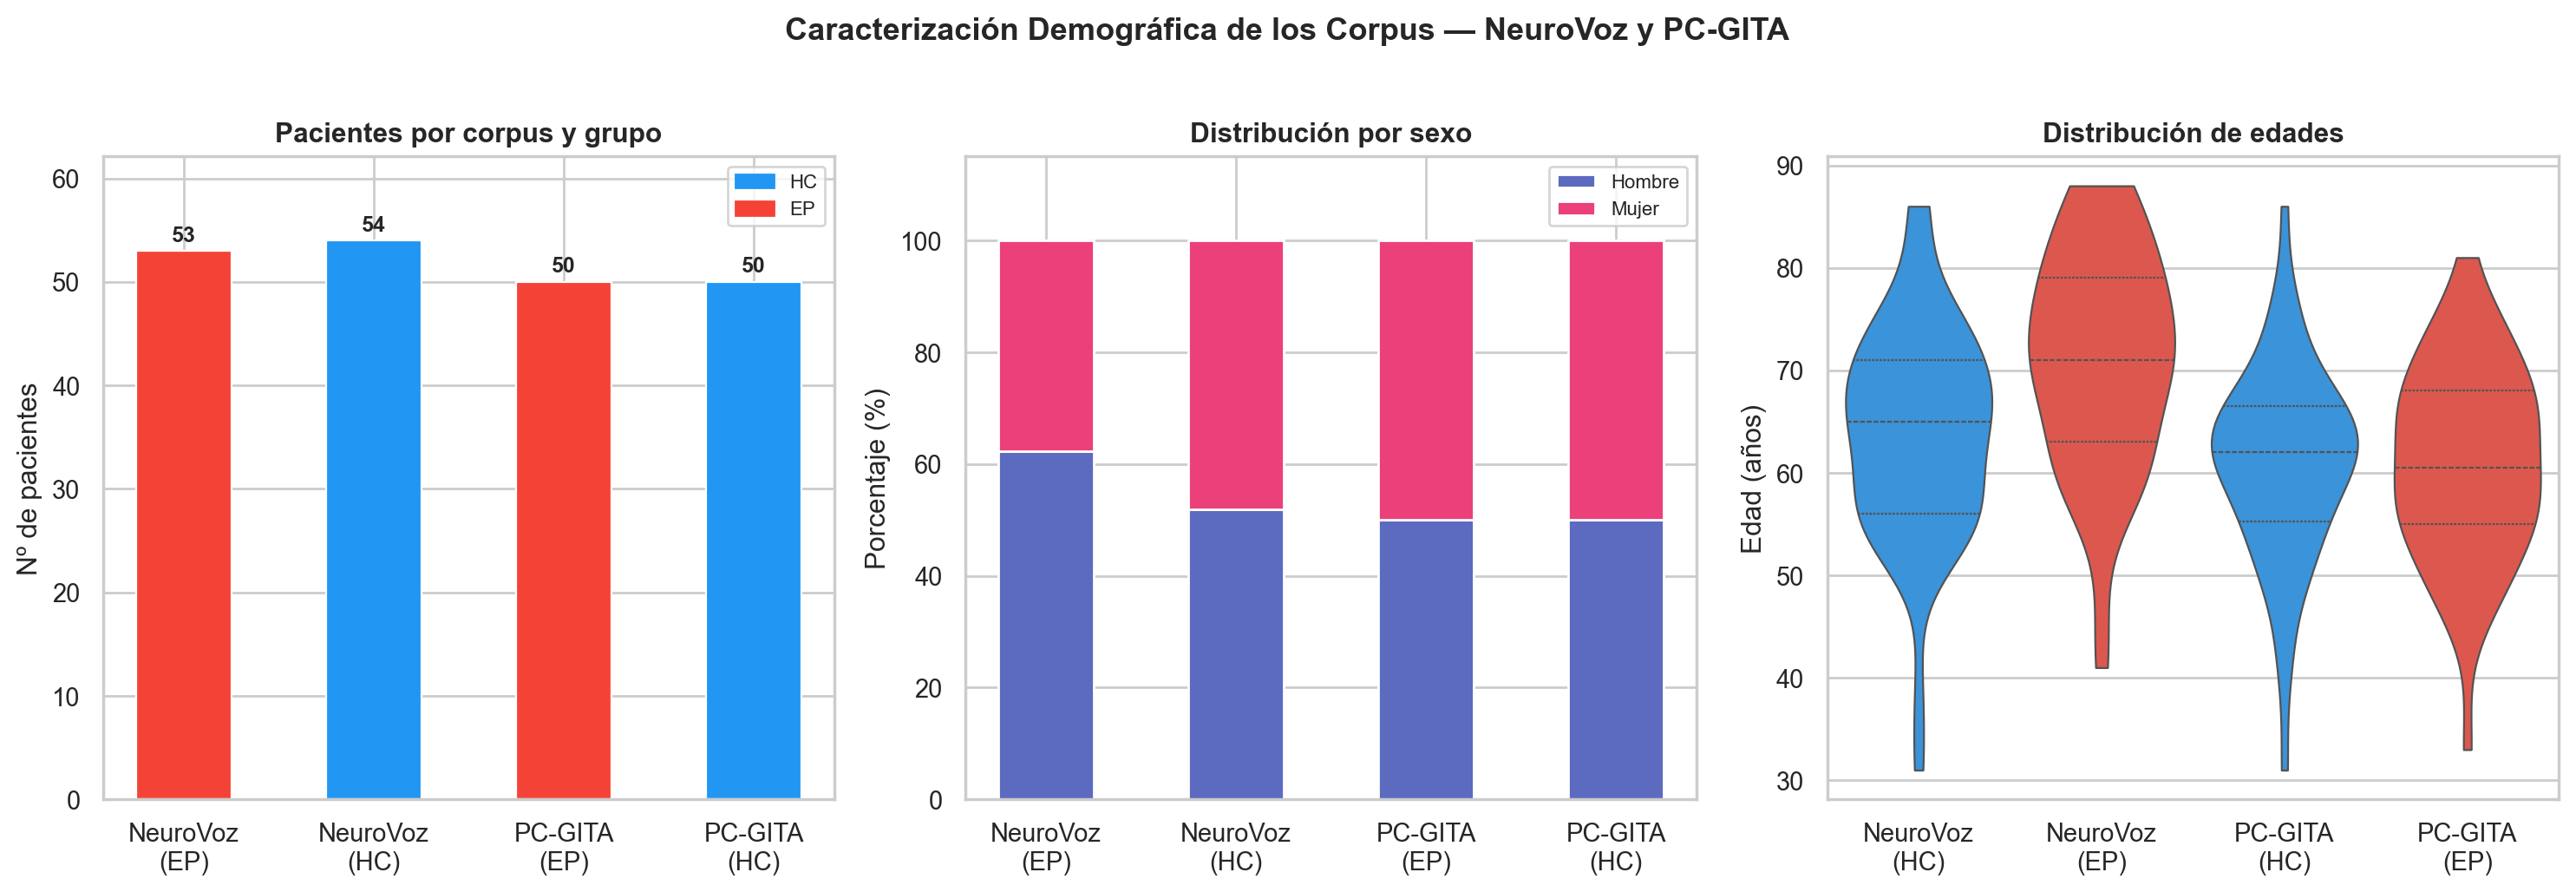
\includegraphics[width=\textwidth]{imagenes/eda/eda_01_demographics.png}
    \caption{Caracterización demográfica de los corpus. De izquierda a derecha: (a) número de pacientes por corpus y grupo diagnóstico; (b) distribución porcentual por sexo; (c) distribución de edades (diagramas de violín con cuartiles internos).}
    \label{fig:eda_demo}
\end{figure}

Se observan dos patrones relevantes. En primer lugar, ambos corpus presentan un ligero predominio masculino, especialmente en el grupo EP de PC-GITA (~70\,\% hombres), lo que refleja la mayor prevalencia de la Enfermedad de Parkinson en varones descrita en la literatura \cite{pringsheim2014}. En segundo lugar, el análisis de las distribuciones de edad revela una diferencia demográfica crítica entre los corpus:

\begin{itemize}
    \item \textbf{NeuroVoz:} el grupo EP presenta una edad media de $71.1 \pm 10.7$ años frente a $64.0 \pm 10.4$ años del grupo HC, lo que supone una diferencia de aproximadamente 7 años. Los grupos \textbf{no están emparejados por edad}, lo que introduce un potencial factor de confusión demográfico: cualquier modelo que incorpore la edad como variable predictora aprenderá, en parte, a predecir la demografía del locutor en lugar del diagnóstico clínico.
    \item \textbf{PC-GITA:} ambos grupos presentan una edad media de $61 \pm 9.4$ y $61 \pm 9.5$ años respectivamente. El corpus está \textbf{perfectamente emparejado por edad} (\textit{age-matched}), lo que lo convierte en el referente metodológico más riguroso para evaluar biomarcadores acústicos independientes del envejecimiento.
\end{itemize}

Esta asimetría motivó la evaluación de modelos con y sin la variable \texttt{Age} como predictor, reportándose los modelos \texttt{sin\_age} (solo características acústicas) como resultados principales por su mayor validez clínica.

\subsection{Distribución de grabaciones por actividad de habla}

La \autoref{fig:eda_recordings} muestra la distribución de grabaciones por actividad y grupo diagnóstico en cada corpus.

\begin{figure}[htbp]
    \centering
    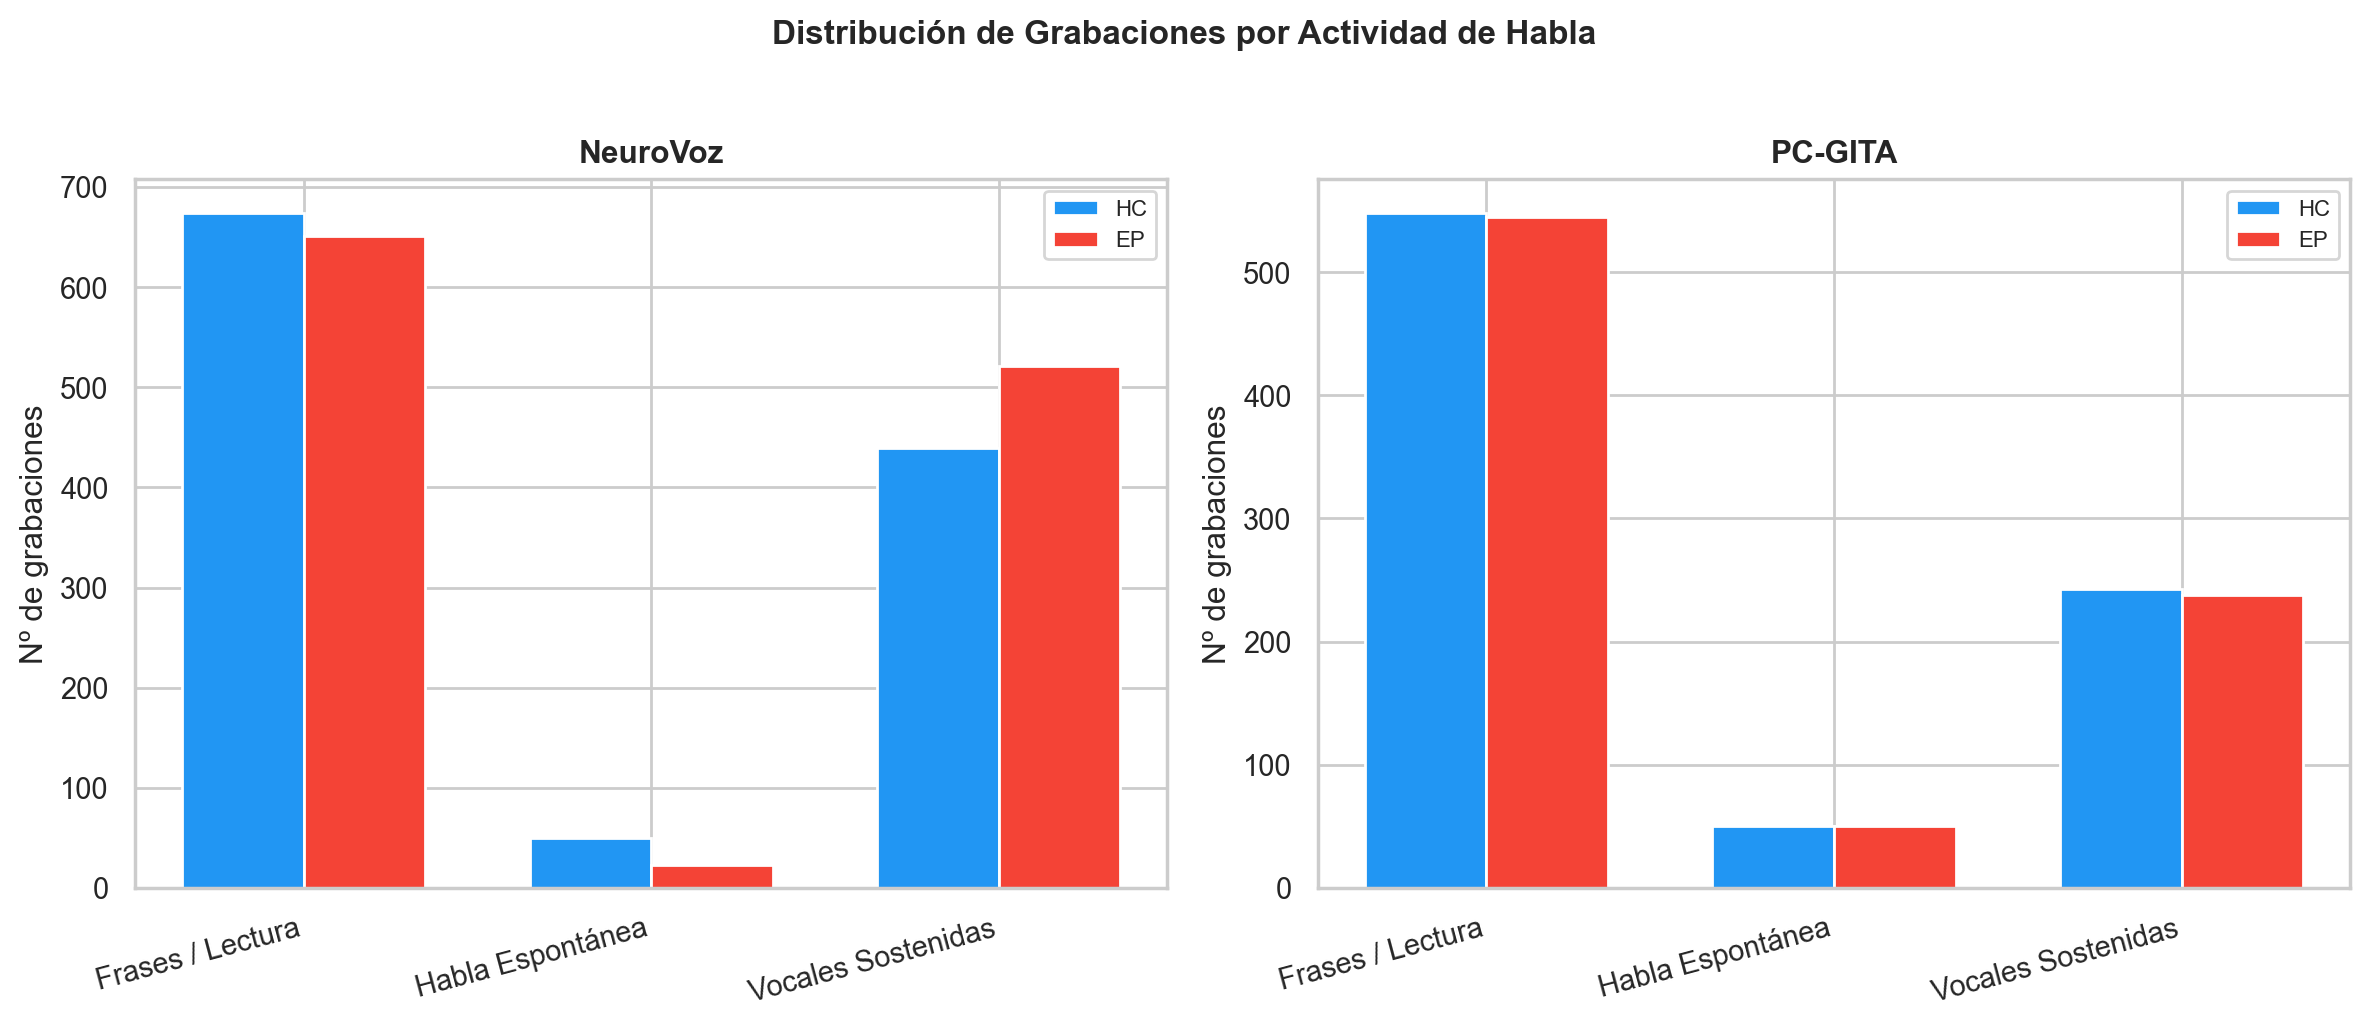
\includegraphics[width=\textwidth]{imagenes/eda/eda_02_recordings.png}
    \caption{Distribución de grabaciones por actividad de habla y grupo diagnóstico en NeuroVoz (izquierda) y PC-GITA (derecha).}
    \label{fig:eda_recordings}
\end{figure}

La actividad de \textbf{Frases / Lectura} es la más abundante en ambos corpus (~1.325 grabaciones en NeuroVoz, ~1.093 en PC-GITA), aportando la mayor potencia estadística para la detección. Las \textbf{Vocales Sostenidas} ocupan el segundo lugar (~960 y ~481 grabaciones respectivamente). El \textbf{Habla Espontánea} es la actividad más escasa y presenta un desequilibrio notable en NeuroVoz: 50 grabaciones HC frente a únicamente 23 EP, situación derivada de diferencias en el protocolo de grabación original del corpus. Este desbalance limita la potencia estadística de los análisis basados en habla espontánea de NeuroVoz y debe considerarse al interpretar los resultados obtenidos con esta modalidad.

% ===========================================================================
\section{Análisis Estadístico de los Biomarcadores Acústicos}
\label{sec:eda_biomarkers}
% ===========================================================================

\subsection{Diagramas de violín por corpus y actividad}

Las Figuras~\ref{fig:violin_nv_vocal}--\ref{fig:violin_pg_esp} muestran las distribuciones de los 16 biomarcadores para los grupos HC (azul) y EP (rojo) en cada una de las seis combinaciones corpus × actividad.

\begin{figure}[p]
    \centering
    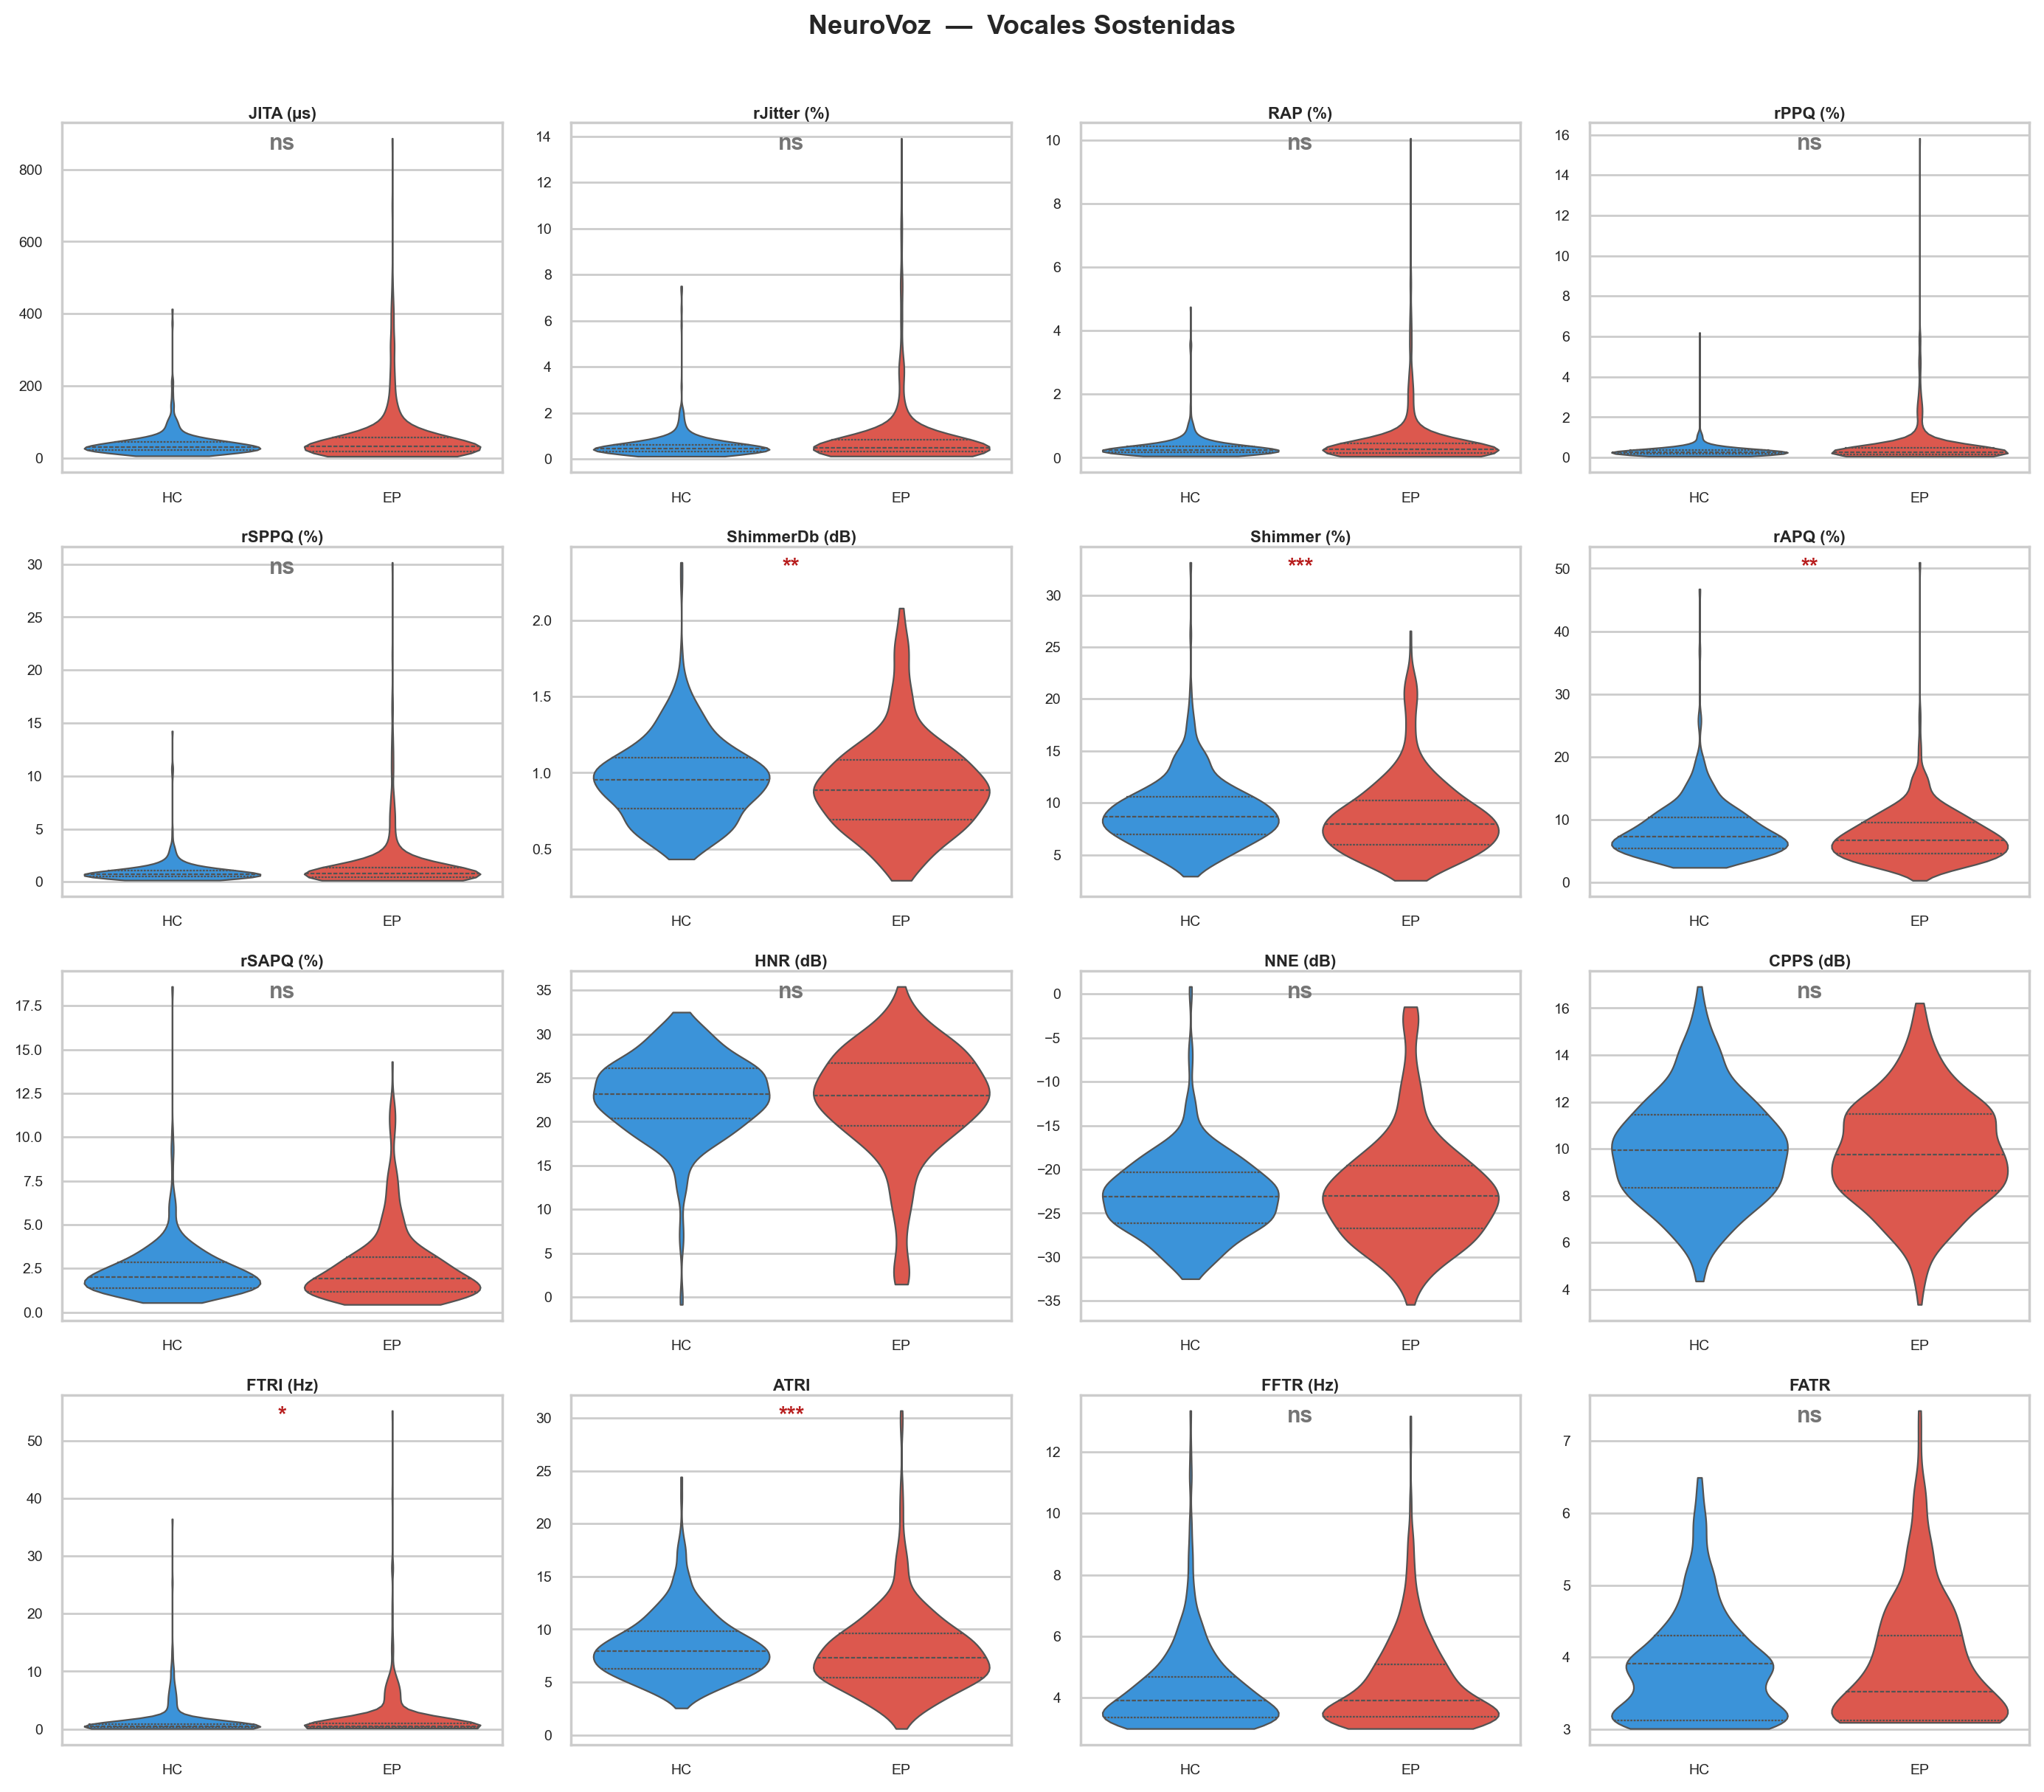
\includegraphics[width=\textwidth, height=0.88\textheight, keepaspectratio]{imagenes/eda/eda_violins_NV_vocal.png}
    \caption{Diagramas de violín — NeuroVoz, Vocales Sostenidas. Las líneas interiores marcan la mediana y los cuartiles Q1/Q3.}
    \label{fig:violin_nv_vocal}
\end{figure}

\begin{figure}[p]
    \centering
    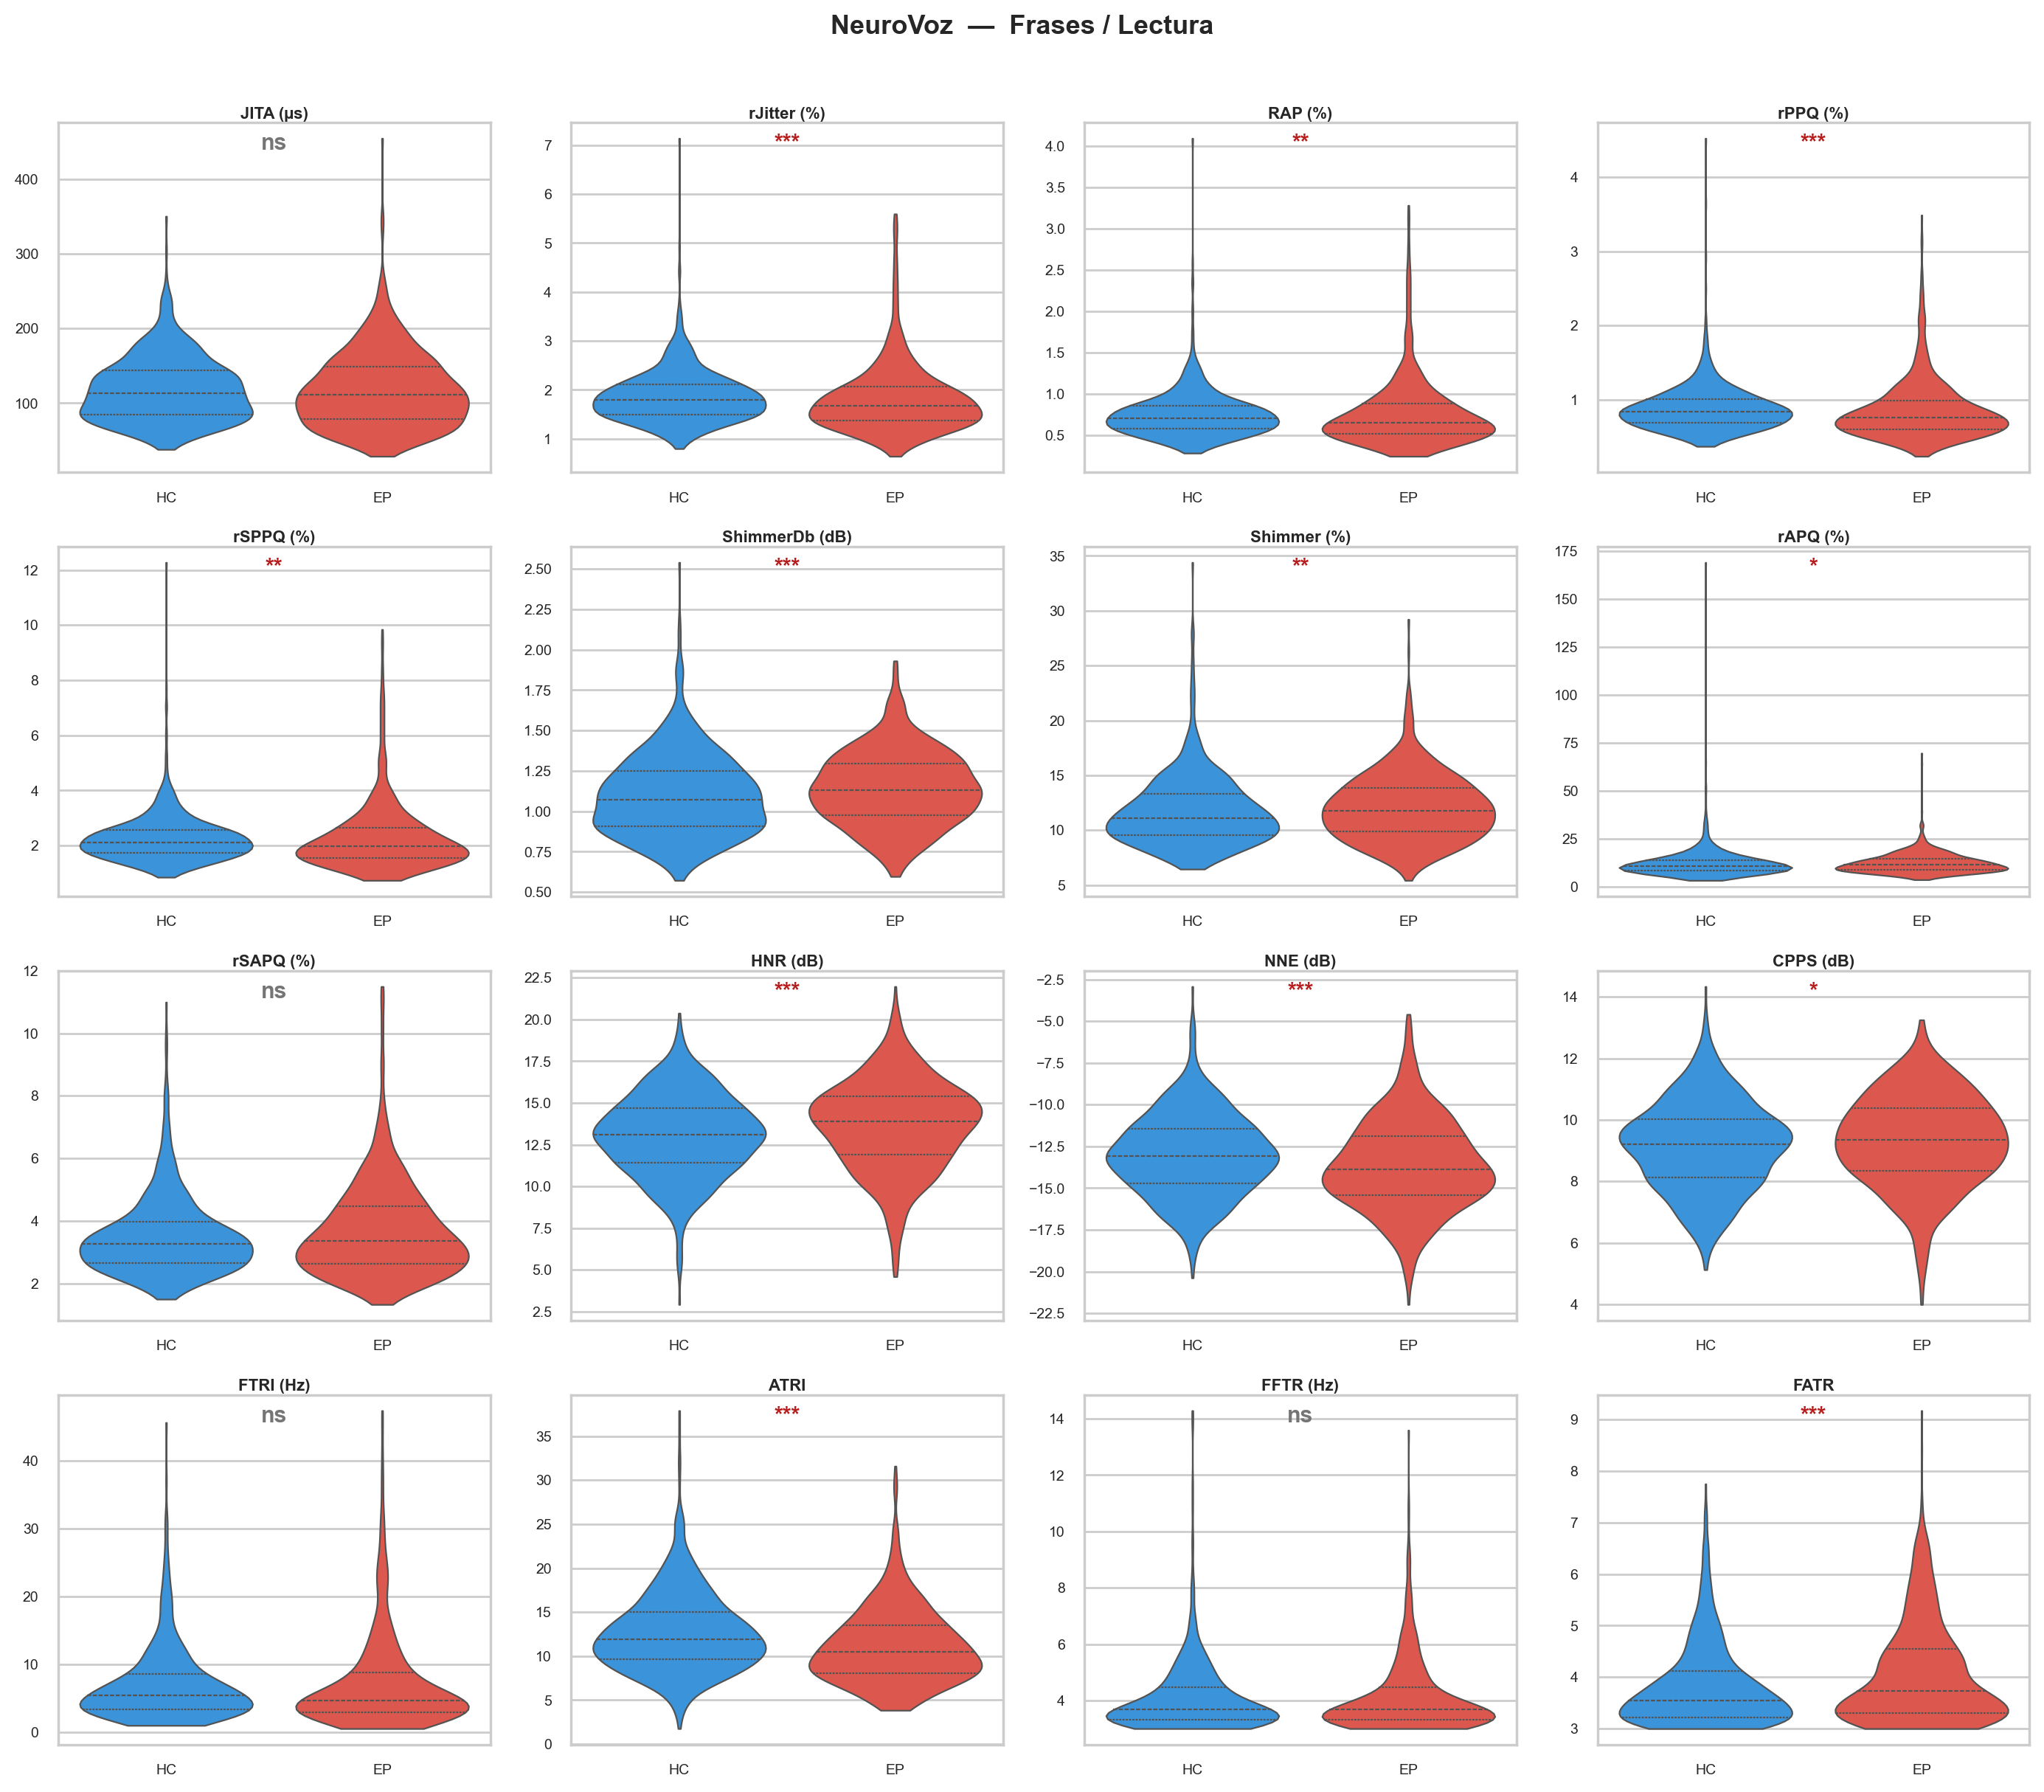
\includegraphics[width=\textwidth, height=0.88\textheight, keepaspectratio]{imagenes/eda/eda_violins_NV_frase.png}
    \caption{Diagramas de violín — NeuroVoz, Frases / Lectura.}
    \label{fig:violin_nv_frase}
\end{figure}

\begin{figure}[p]
    \centering
    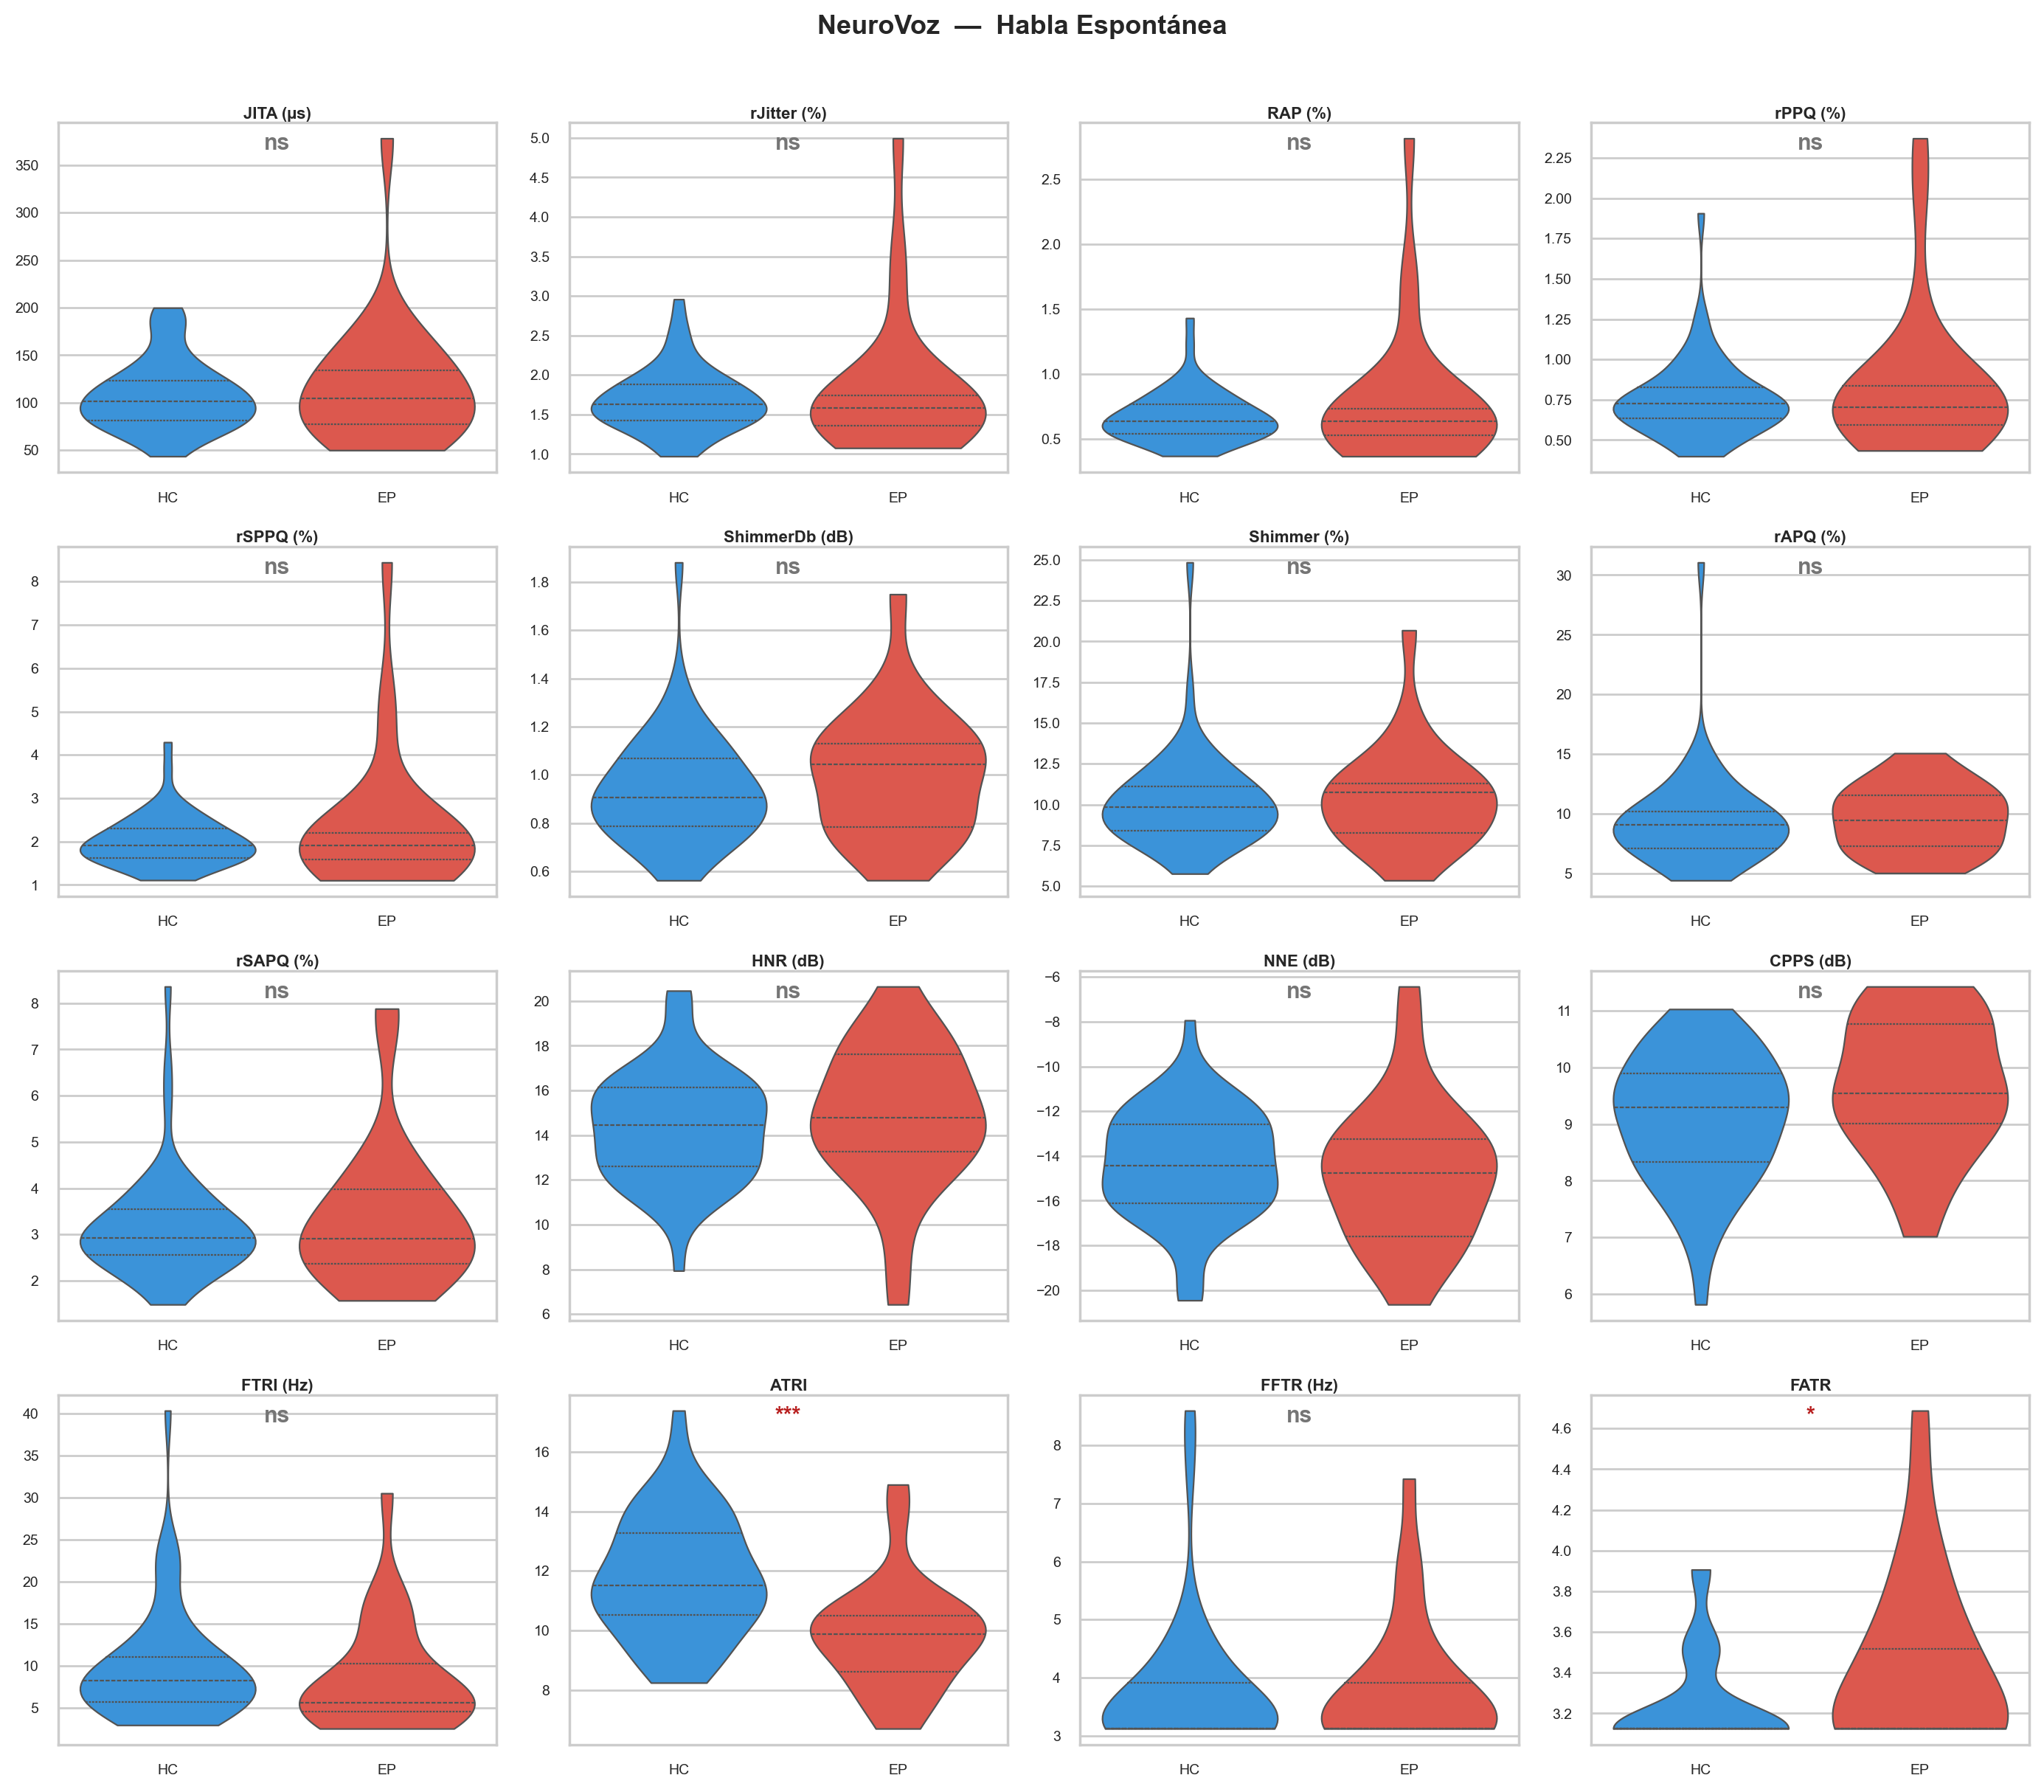
\includegraphics[width=\textwidth, height=0.88\textheight, keepaspectratio]{imagenes/eda/eda_violins_NV_espontanea.png}
    \caption{Diagramas de violín — NeuroVoz, Habla Espontánea. La mayoría de biomarcadores resulta no significativo por el reducido N del grupo EP (23 grabaciones).}
    \label{fig:violin_nv_esp}
\end{figure}

\begin{figure}[p]
    \centering
    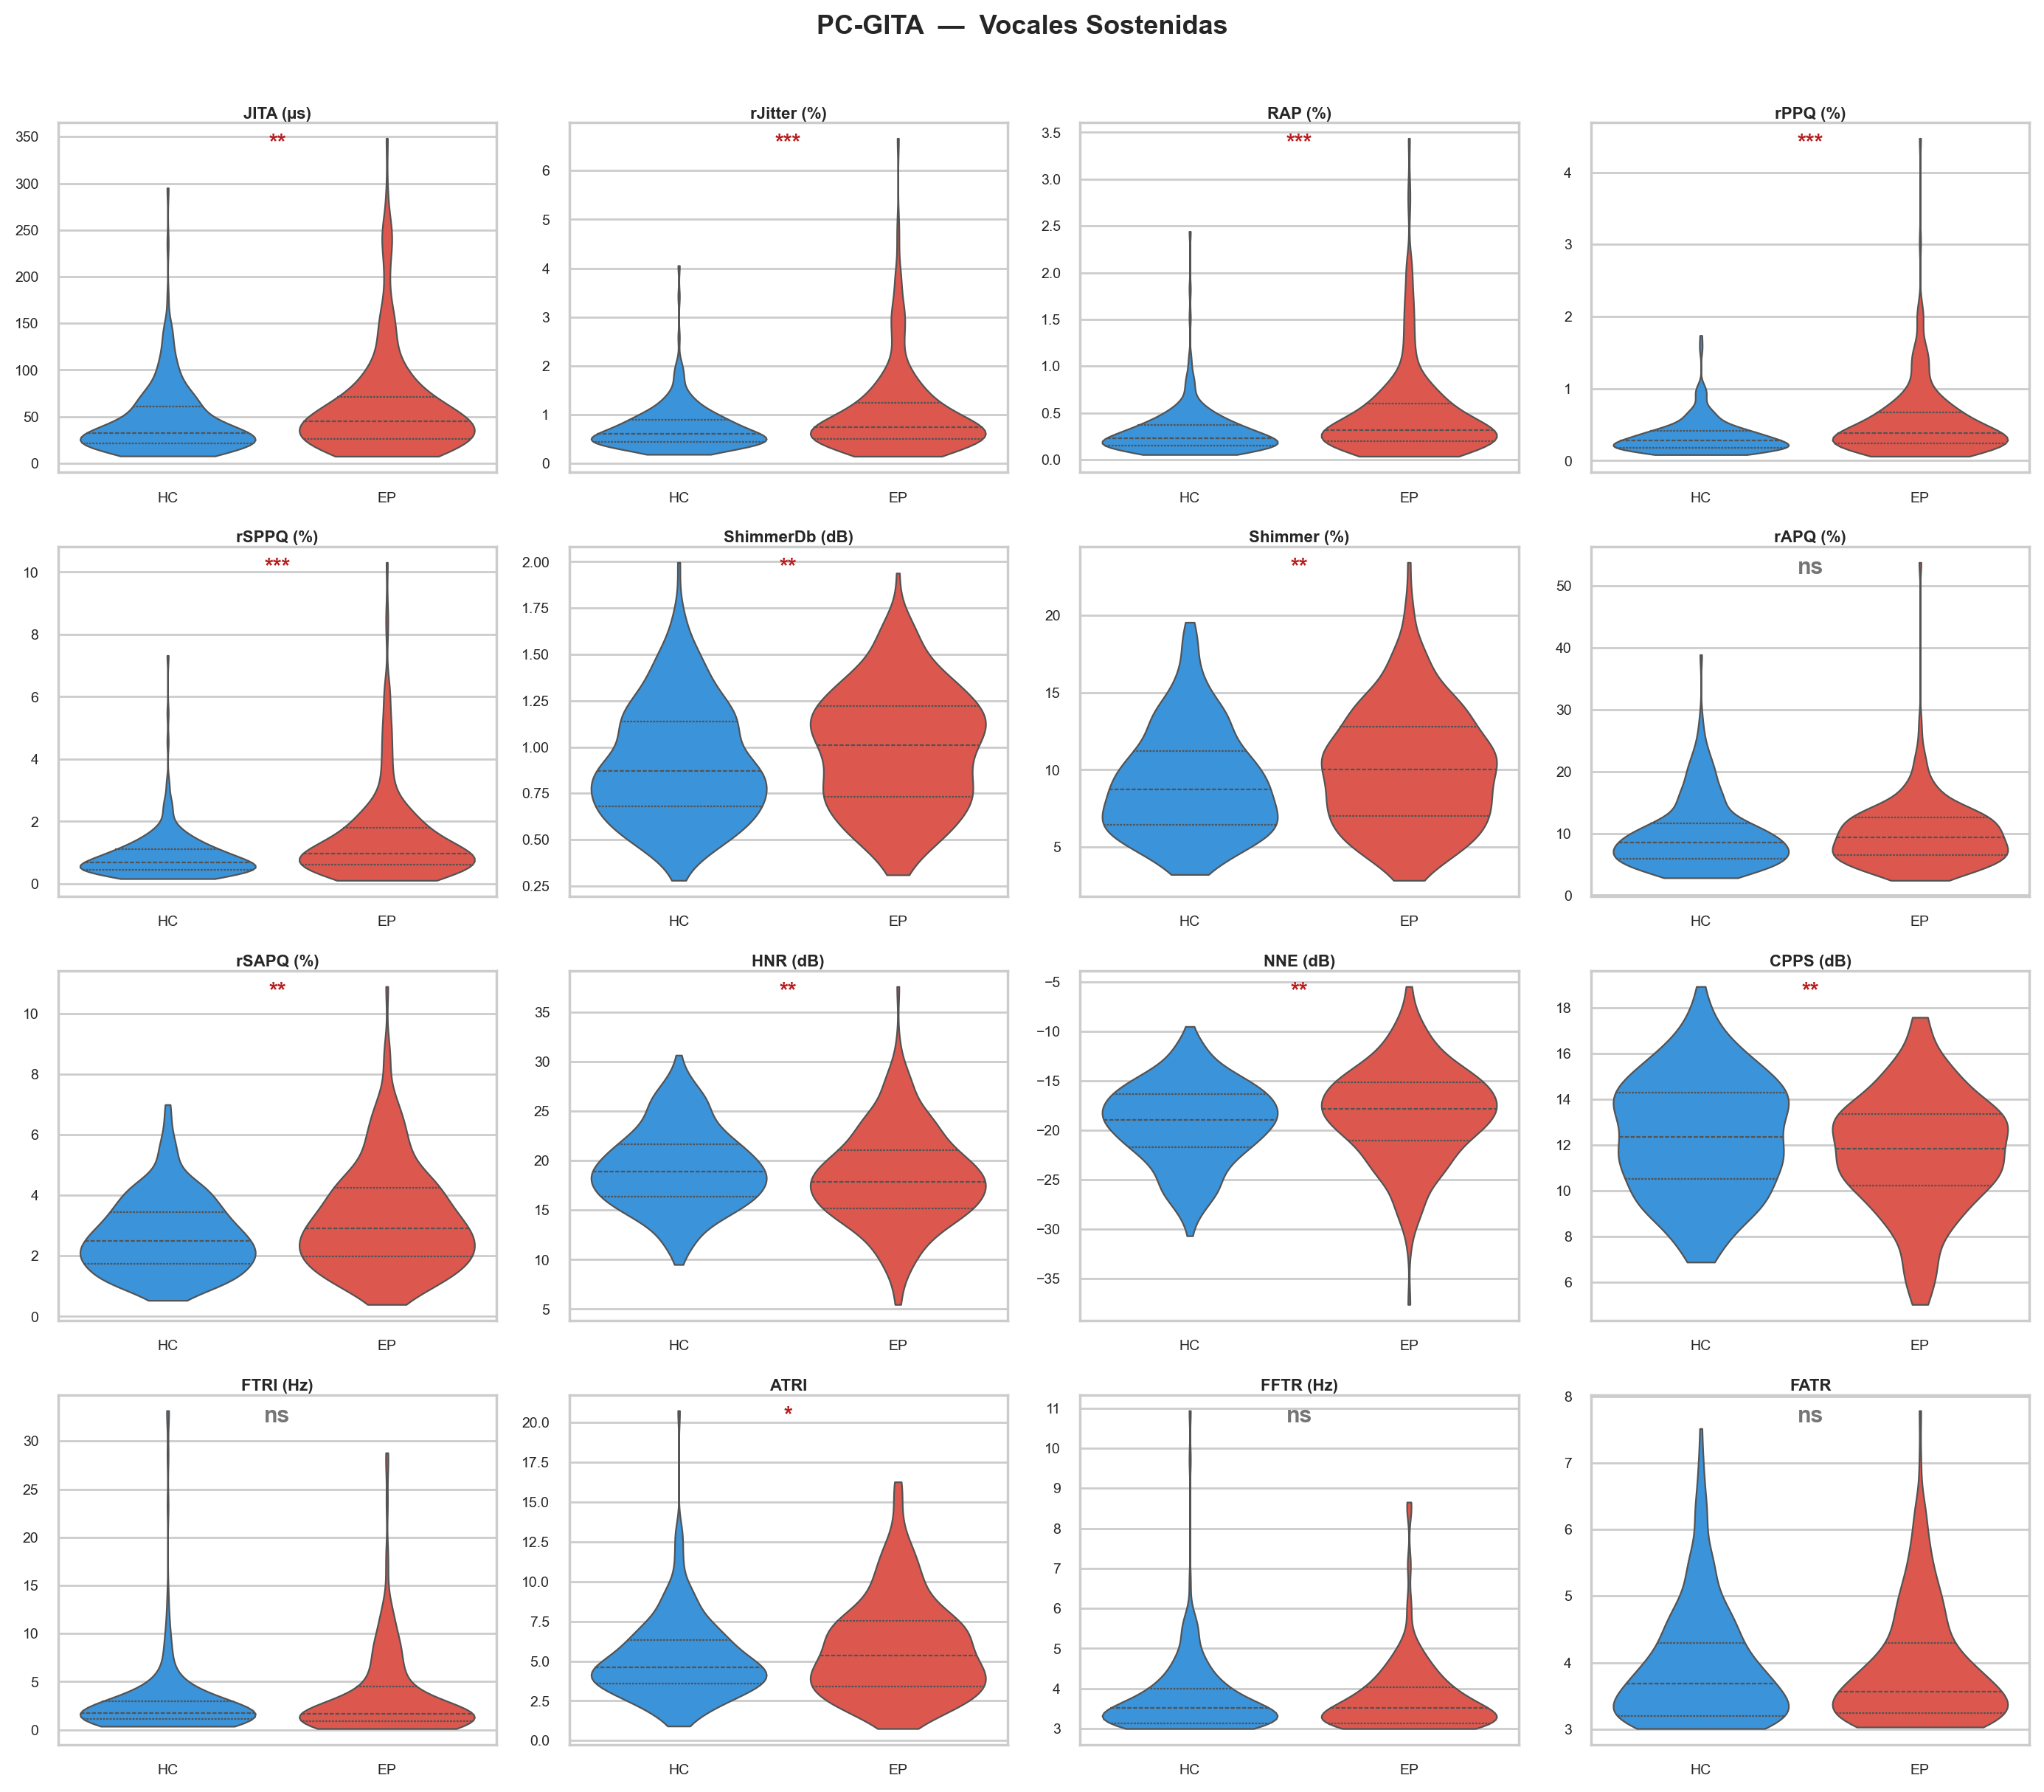
\includegraphics[width=\textwidth, height=0.88\textheight, keepaspectratio]{imagenes/eda/eda_violins_PG_vocal.png}
    \caption{Diagramas de violín — PC-GITA, Vocales Sostenidas.}
    \label{fig:violin_pg_vocal}
\end{figure}

\begin{figure}[p]
    \centering
    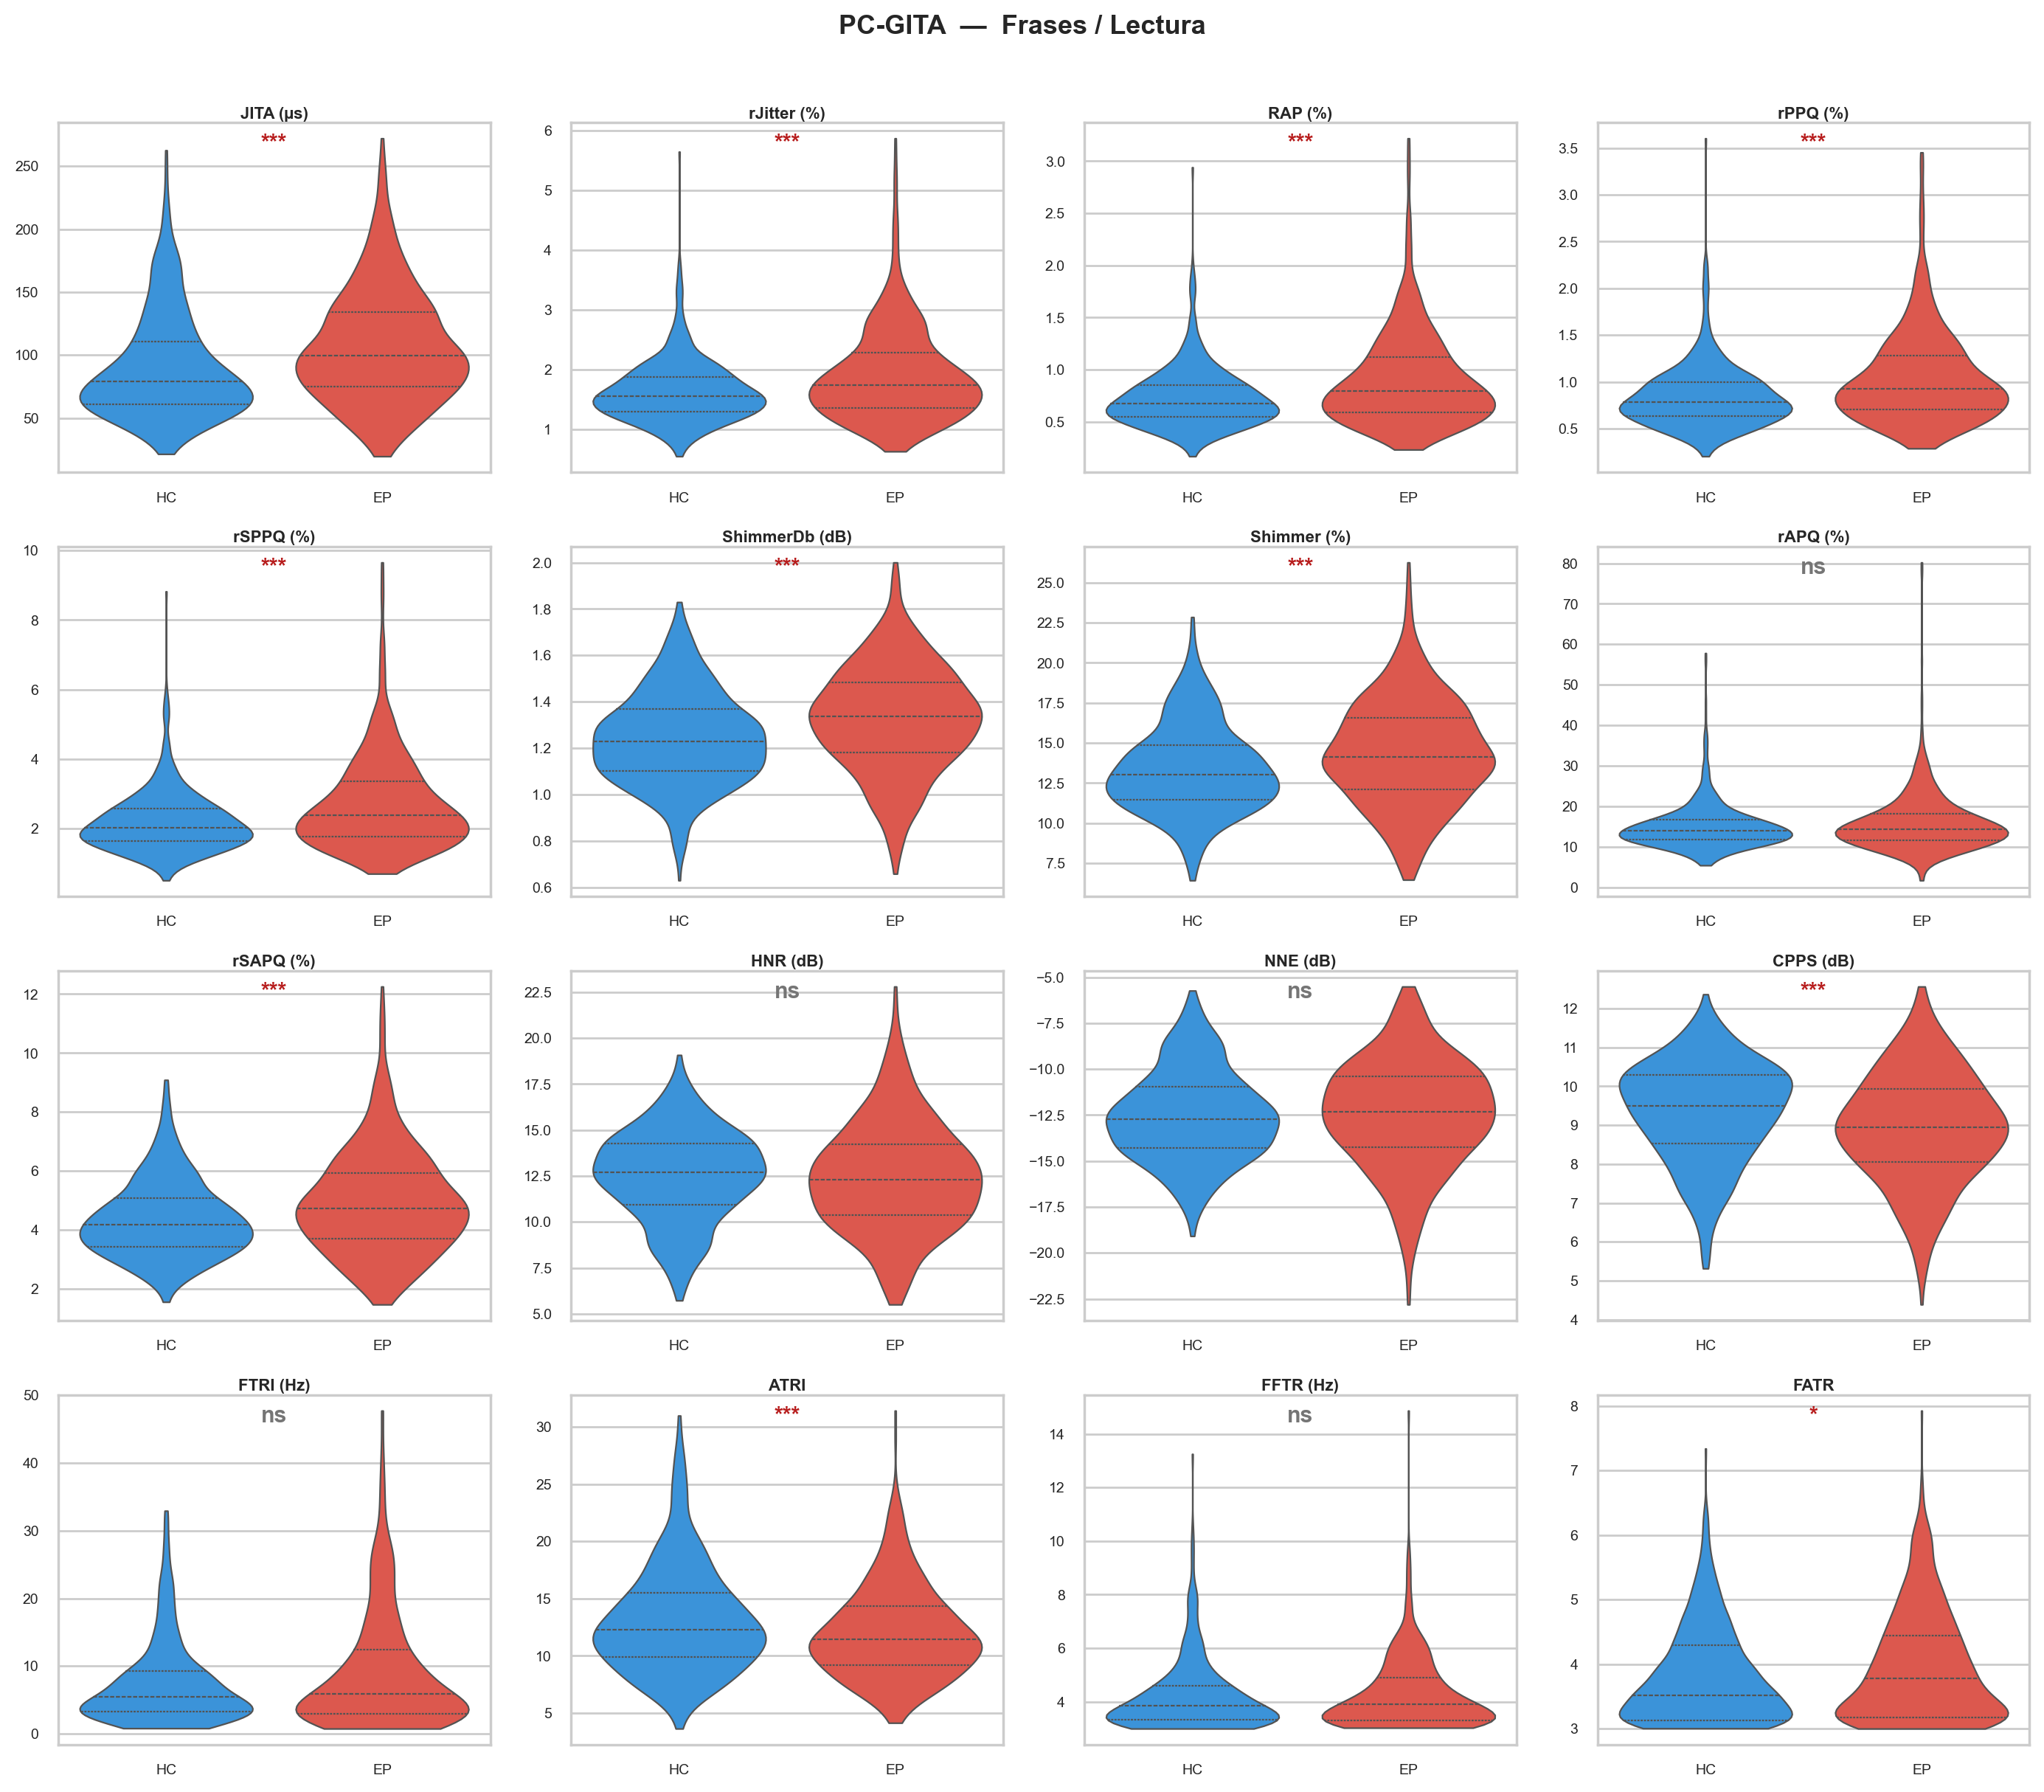
\includegraphics[width=\textwidth, height=0.88\textheight, keepaspectratio]{imagenes/eda/eda_violins_PG_frase.png}
    \caption{Diagramas de violín — PC-GITA, Frases / Lectura. Esta condición presenta las separaciones más pronunciadas entre grupos en todo el conjunto de datos.}
    \label{fig:violin_pg_frase}
\end{figure}

\begin{figure}[p]
    \centering
    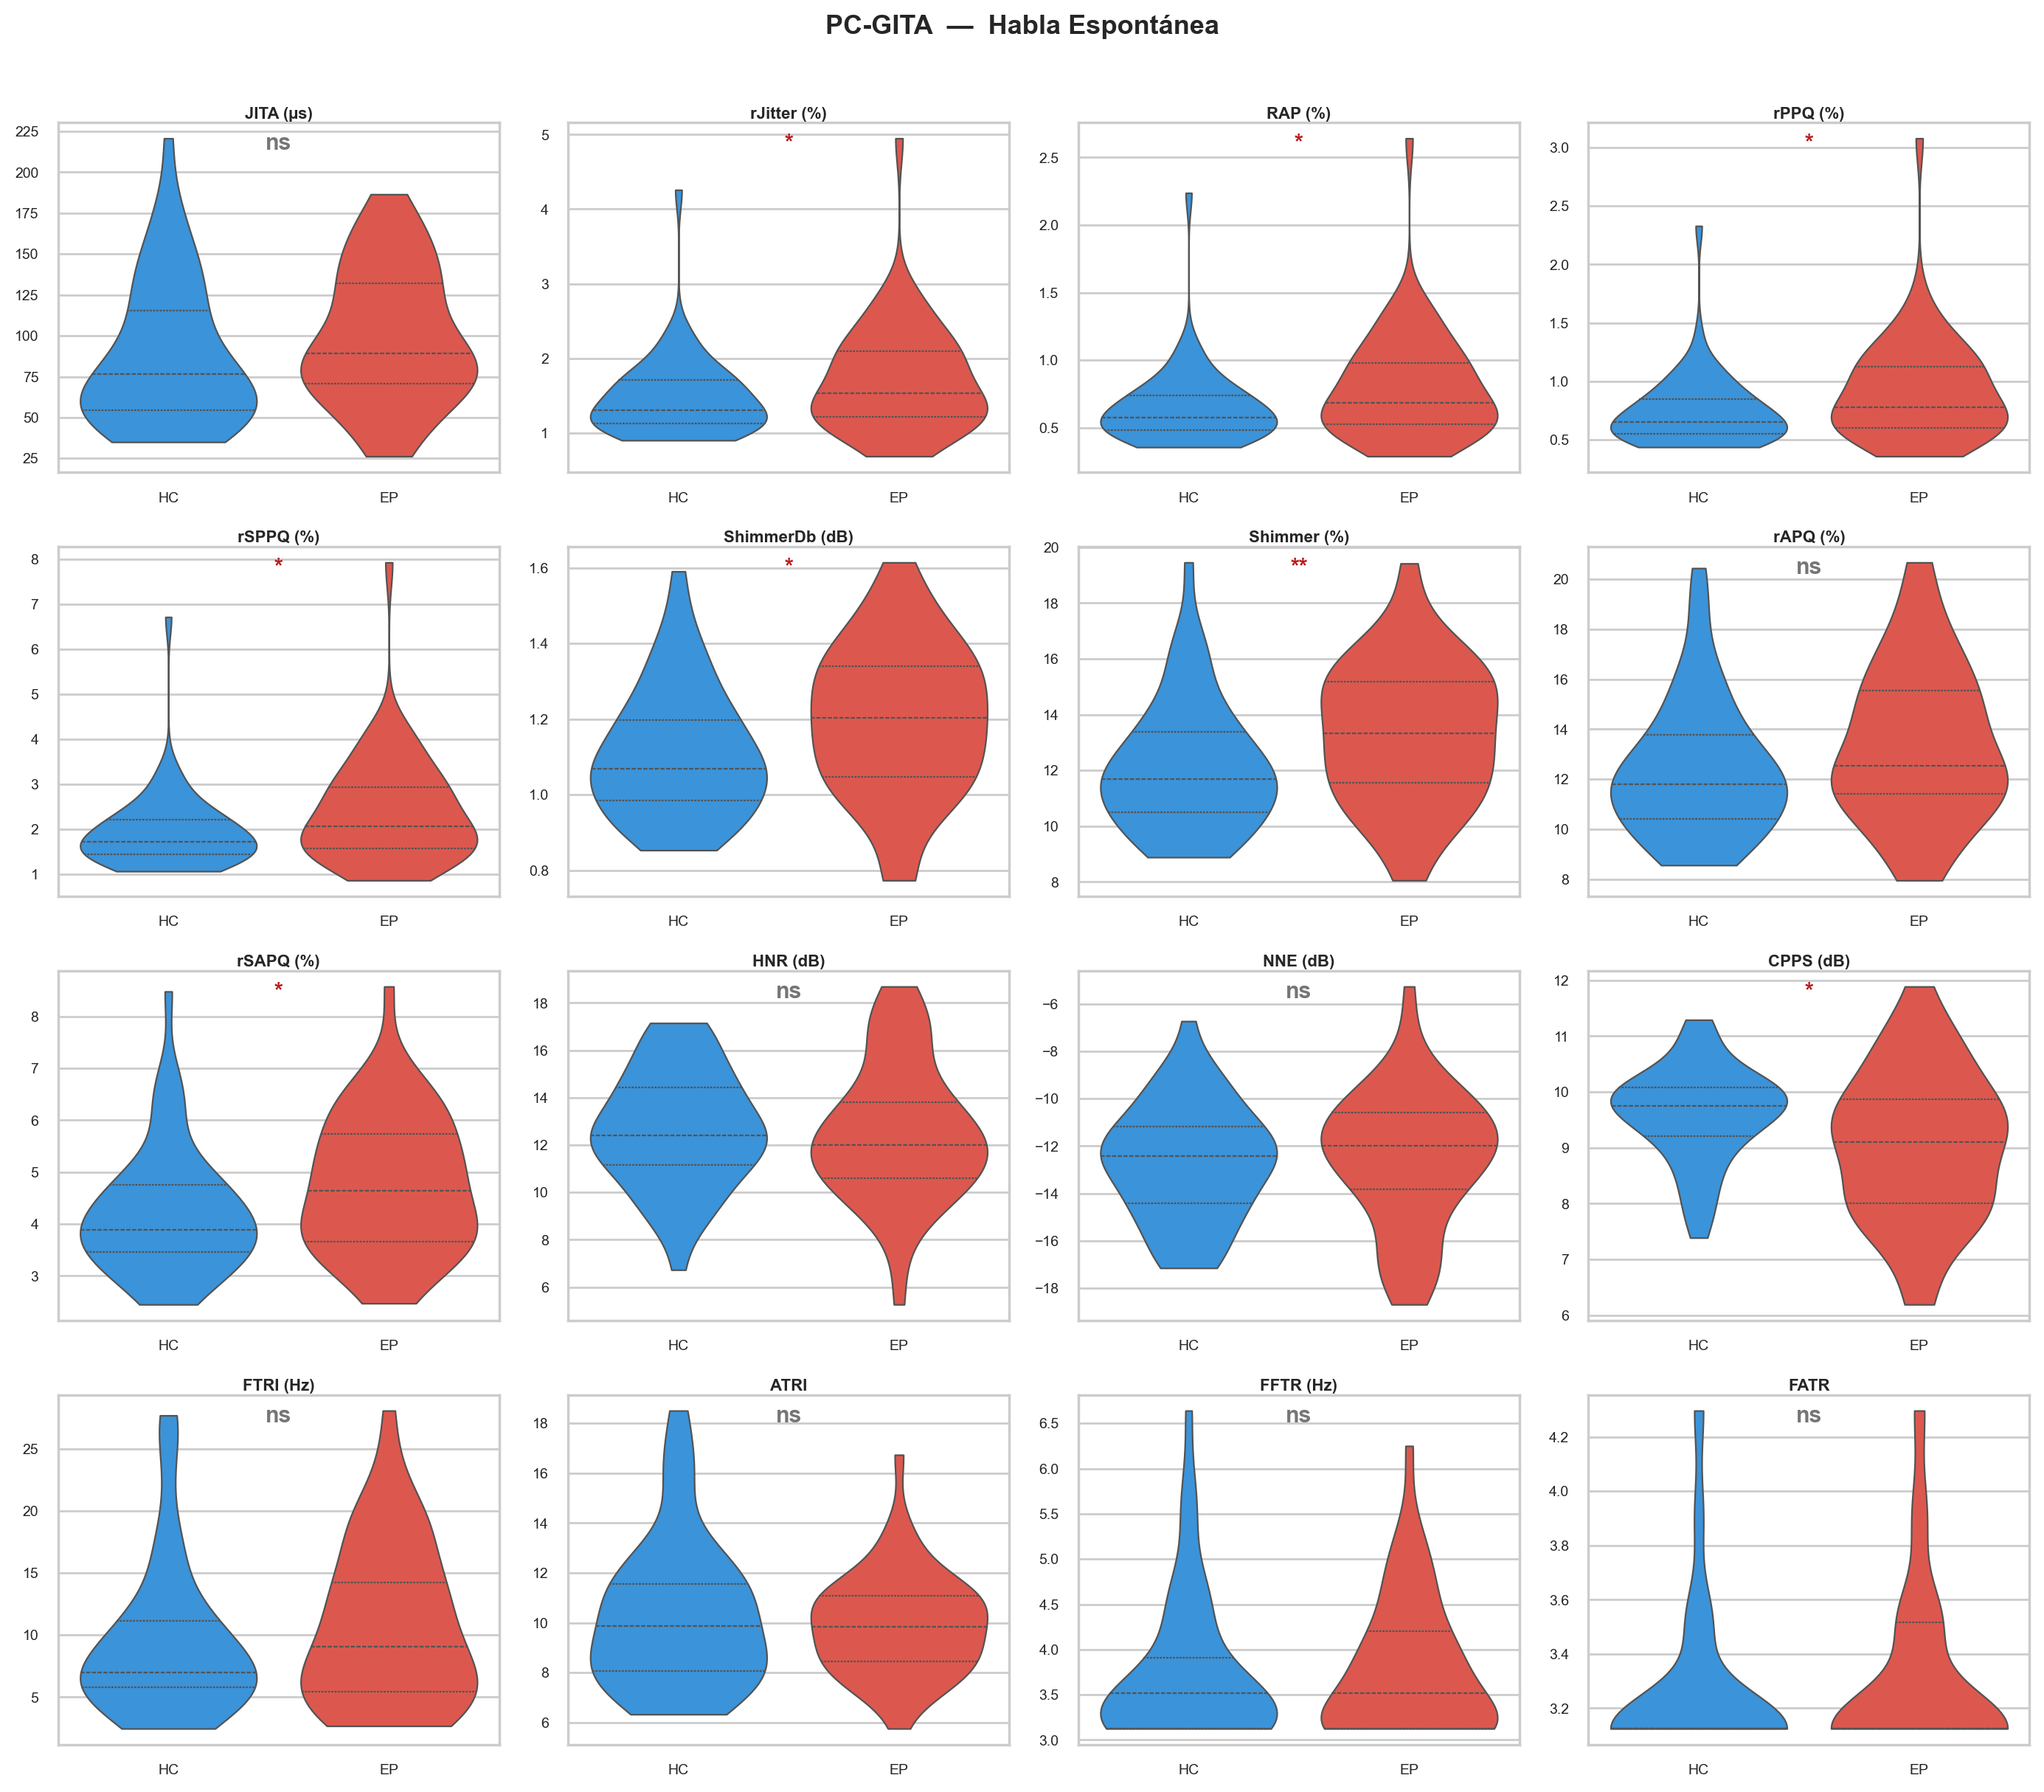
\includegraphics[width=\textwidth, height=0.88\textheight, keepaspectratio]{imagenes/eda/eda_violins_PG_espontanea.png}
    \caption{Diagramas de violín — PC-GITA, Habla Espontánea.}
    \label{fig:violin_pg_esp}
\end{figure}

De la inspección de los diagramas de violín se extraen las siguientes conclusiones por tipo de biomarcador:

\paragraph{Jitter (perturbación de frecuencia).} En \textbf{PC-GITA Vocales} y \textbf{PC-GITA Frases}, todas las variantes de jitter (JITA, rJitter, RAP, rPPQ, rSPPQ) presentan una separación clara: los violines EP están desplazados hacia valores más altos y son más dispersos, reflejando la irregularidad en el control del periodo fundamental. Sorprendentemente, en \textbf{NeuroVoz Vocales} estas mismas métricas no resultan significativas, lo que sugiere diferencias en el protocolo de grabación o en las características de los participantes entre los dos corpus.

\paragraph{Shimmer (perturbación de amplitud).} ShimmerDb y Shimmer son significativos en \textbf{PC-GITA Frases} con una separación muy pronunciada, y en \textbf{NeuroVoz Frases} de forma moderada. En vocales, la separación es menor pero presente, especialmente en PC-GITA. Esto indica que la inestabilidad en la amplitud vocal de los pacientes EP es más manifiesta durante la lectura de frases que en la fonación sostenida.

\paragraph{Armonicidad (HNR, NNE, CPPS).} HNR y NNE destacan en \textbf{NeuroVoz Frases}: los violines HC se concentran en valores altos (voz limpia), mientras que EP se extiende hacia valores menores (mayor componente ruidoso). CPPS presenta significancia en \textbf{PC-GITA Frases} y \textbf{PC-GITA Vocales}, siendo coherente con los resultados del análisis de importancia Random Forest que lo sitúa como el biomarcador más relevante en habla espontánea.

\paragraph{Temblor (ATRI).} ATRI muestra la separación más consistente del conjunto: en \textbf{NeuroVoz Frases} y \textbf{NeuroVoz Vocales} los violines EP son notablemente más amplios y desplazados hacia valores más altos, reflejando el temblor fonatorio de baja frecuencia (3--15\,Hz) característico de la disartria hipocinética parkinsoniana. Es el único biomarcador con separación visible incluso en habla espontánea pese al reducido N.

    \chapter{Dependencias del entorno virtual}
\label{app:anexo_entorno} 

En este anexo se detalla la configuración exacta del entorno de software utilizado para el desarrollo, entrenamiento y despliegue de los modelos de inteligencia artificial del proyecto. La gestión del entorno se ha llevado a cabo mediante el gestor de dependencias \texttt{uv}.

\section*{Entorno base}
\begin{itemize}
    \item \textbf{Lenguaje principal:} Python 3.11.14
    \item \textbf{Gestor de paquetes:} uv
\end{itemize}

\section*{Listado de librerías}
A continuación, se expone el listado exhaustivo de las dependencias principales requeridas para la correcta ejecución del código fuente, tal y como se especificarían en el archivo de configuración del proyecto:

\begin{verbatim}
fastapi>=0.135.1
ipykernel>=7.2.0
joblib>=1.5.3
jupyter>=1.1.1
librosa>=0.11.0
matplotlib>=3.10.8
noisereduce>=3.0.3
numpy>=2.4.2
pandas>=3.0.1
praat-parselmouth>=0.4.7
python-multipart>=0.0.22
scikit-learn>=1.8.0
scipy>=1.17.0
seaborn>=0.13.2
shap>=0.49.1
timm>=1.0.25
torch>=2.6.0
torchvision>=0.20.0
torchaudio>=2.6.0
tqdm>=4.67.3
uvicorn>=0.41.0
xgboost==2.0.3
openpyxl>=3.1.5
transformers>=5.7.0
\end{verbatim}
    \chapter{Repositorio y Binarios de la Aplicación}
\label{app:anexo_b} 

Lorem Ipsum
"Neque porro quisquam est qui dolorem ipsum quia dolor sit amet, consectetur, adipisci velit..."
"There is no one who loves pain itself, who seeks after it and wants to have it, simply because it is pain..."

Lorem ipsum dolor sit amet, consectetur adipiscing elit. Nunc suscipit sodales interdum. Sed aliquam enim sit amet pellentesque facilisis. Vivamus pretium vitae dolor in elementum. Etiam lacinia tortor metus, sit amet tincidunt massa porta ut. In ut massa convallis, congue augue ac, tempor ante. Nunc luctus sapien nec libero facilisis vulputate. Fusce tincidunt quam dui. Ut suscipit fermentum lacus, nec facilisis arcu sollicitudin non. Proin gravida tortor egestas, sagittis turpis ut, porta lacus. Morbi posuere viverra pellentesque.

Pellentesque sodales arcu sit amet nisl sollicitudin tincidunt. Nam quis arcu ipsum. Aliquam ornare ut velit sit amet imperdiet. Phasellus dignissim, quam ac convallis vehicula, purus ipsum placerat arcu, ac aliquam turpis ligula eu justo. Donec a nisi pharetra dolor porta molestie nec eu turpis. Cras feugiat ex ac dictum condimentum. Nulla vestibulum faucibus laoreet. Proin quis pharetra dui. Suspendisse iaculis enim sed pellentesque porta. Nam neque leo, euismod ac maximus a, maximus sed sem. Etiam vitae nibh vitae neque faucibus ultrices nec ut orci. Etiam feugiat, arcu nec rutrum accumsan, purus dui vestibulum dui, et maximus turpis leo vel sapien. Class aptent taciti sociosqu ad litora torquent per conubia nostra, per inceptos himenaeos.

Proin id nunc lorem. Donec et dui turpis. Nam et ante tempus, cursus orci non, consectetur ligula. Vivamus at urna purus. Praesent eget fringilla enim, non luctus leo. Pellentesque habitant morbi tristique senectus et netus et malesuada fames ac turpis egestas. Etiam ullamcorper, arcu eu lobortis ornare, dolor purus ultrices nisi, ut pharetra ante arcu nec nibh. Fusce consequat a risus a pulvinar.

Vivamus tristique commodo nunc ut molestie. Vivamus eget sapien tortor. Nam dui odio, facilisis non consectetur vitae, imperdiet at odio. Mauris vitae lorem id dolor euismod scelerisque eu a libero. Morbi euismod erat iaculis ipsum aliquam euismod. Ut porttitor viverra neque scelerisque rhoncus. Etiam pulvinar risus ac porta ornare. Nulla tempor feugiat sem, eu mollis lacus suscipit et.

Etiam mi massa, sagittis a arcu a, blandit dignissim purus. Ut suscipit quis risus non rutrum. Nunc sollicitudin nulla ut aliquet consequat. Maecenas imperdiet, urna id laoreet gravida, ligula nunc hendrerit mi, ut posuere neque odio non tortor. Proin accumsan tristique dolor eget bibendum. Mauris vulputate sit amet enim tincidunt convallis. Nunc at sem nibh. Vivamus eget elit pretium, cursus lectus sed, venenatis erat. Donec lectus urna, venenatis id ex eu, tempus dapibus ligula. Nulla aliquet felis vitae vulputate pulvinar. Mauris non interdum tellus. Quisque metus justo, iaculis vitae tristique in, lacinia id dolor. Maecenas ultrices ultricies mauris vitae condimentum. Nulla nulla urna, pellentesque quis eros a, congue rhoncus lectus.




    

\end{document}